%\documentclass[utf8]{book}
\documentclass[10.5pt,a4paper]{ctexbook} % 五号字,A4


%========== 包 ==========
%\usepackage[UTF8]{ctex}                   % chinese
\usepackage{anyfontsize}                  % 10.5pt in ctexbook
\usepackage{booktabs}                     % \newpage
\usepackage{tcolorbox}                    % frame box
\usepackage{enumitem}                     % item
\usepackage{graphicx}                     % images
\usepackage{amsmath, amsthm, amssymb, bm} % math
\usepackage{hyperref, mathrsfs}           % ref
\usepackage{esint}                        % closed geometry integral symbol
\usepackage{pgfplots, tikz}               % tikzpicture
\usetikzlibrary{patterns,arrows,positioning,calc,fadings,shapes,decorations.markings,intersections,through,angles,quotes,decorations.pathreplacing,calligraphy}


%========== 环境 ==========
\newtheorem{definition}{定义}[section]
\newtheorem{example}{例}[section]
\newtheorem{theorem}{定理}[section]
\newtheorem{lemma}[theorem]{引理}
\newtheorem{corollary}[theorem]{推论}
\newtheorem{proposition}[theorem]{命题}


%========== enum和item设置 ==========
%\ctexset{section={beforeskip=50.0ex plus 0.2ex minus .2ex}}
%\ctexset{section={beforeskip=\doublespace}}
%\ctexset{section={format=\heiti\centering\zihao{-3},beforeskip=20cm},subsection={beforeskip=6ex}}
\ctexset{section={beforeskip=5ex},subsection={beforeskip=5ex}}
\setcounter{secnumdepth}{3}
\setcounter{tocdepth}{3}
\setenumerate[1]{itemsep=0pt,partopsep=0pt,parsep=\parskip,topsep=0pt,left=\parindent}
\setitemize[1]{itemsep=0pt,partopsep=0pt,parsep=\parskip,topsep=0pt,left=\parindent}
\setdescription{itemsep=0pt,partopsep=0pt,parsep=\parskip,topsep=5pt}
\graphicspath{{./figures}}


%%% \mydrawxy{x_lim_left}{x_lim_right}{y_lim_left}{y_lim_right}
\newcommand \mydrawxy[4]
{
\coordinate (x1) at (#1,0);
\coordinate (y1) at (0,#3);
\coordinate[label=right:{$x$}] (x2) at (#2,0);
\coordinate[label=above:{$y$}] (y2) at (0,#4);
\draw[->,red] (x1)--(x2);
\draw[->,red] (y1)--(y2);
}

%%% \mydrawsquare[length=1]{A}{B}{C}{D}
\newcommand \mydrawsquare[5][1]
{
\coordinate[label=left: {$#2$}] (#2) at (0,0);            % A
\coordinate[label=right:{$#3$}] (#3) at ($(#2)+(#1,0)$);  % B
\coordinate[label=right:{$#4$}] (#4) at ($(#2)+(#1,#1)$); % C
\coordinate[label=left: {$#5$}] (#5) at ($(#2)+(0,#1)$);  % D
\draw[thick] (#2)--(#3)--(#4)--(#5)--(#2);
}

%%% \mydrawxyz{x_lim_left}{x_lim_right}{y_lim_left}{y_lim_right}{z_lim_left}{z_lim_right}
\newcommand \mydrawxyz[6]
{
\coordinate (x1) at (#1,0,0);
\coordinate (y1) at (0,#3,0);
\coordinate (z1) at (0,0,#5);
\coordinate[label=below left:{$x$}] (x2) at (#2,0,0);
\coordinate[label=right:     {$y$}] (y2) at (0,#4,0);
\coordinate[label=above:     {$z$}] (z2) at (0,0,#6);
\draw[->,red] (x1)--(x2);
\draw[->,red] (y1)--(y2);
\draw[->,red] (z1)--(z2);
}

%%% \mydrawcube[length=1]{A}{B}{C}{D}{A'}{B'}{C'}{D'}
\newcommand \mydrawcube[9][1]
{
\coordinate[label=left: {$#2$}] (#2) at (0,0,0);             % A
\coordinate[label=right:{$#3$}] (#3) at ($(#2)+(0,#1,0)$);   % B
\coordinate[label=right:{$#4$}] (#4) at ($(#2)+(-#1,#1,0)$); % C
\coordinate[label=left: {$#5$}] (#5) at ($(#2)+(-#1,0,0)$);  % D
\coordinate[label=left: {$#6$}] (#6) at ($(#2)+(0,0,#1)$);   % A'
\coordinate[label=right:{$#7$}] (#7) at ($(#6)+(0,#1,0)$);   % B'
\coordinate[label=right:{$#8$}] (#8) at ($(#6)+(-#1,#1,0)$); % C'
\coordinate[label=left: {$#9$}] (#9) at ($(#6)+(-#1,0,0)$);  % D'
\draw[thick] (#6)--(#9)--(#8)--(#4)--(#3);                   % A'-D'-C'-C-B
\draw[thick] (#7)--(#6)--(#2)--(#3)--(#7)--(#8);             % B'-A'-A-B-B'-C'
\draw[dashed] (#2)--(#5);
\draw[dashed] (#9)--(#5)--(#4);
}


%========== 文档 ==========
\raggedbottom
\begin{document}


%========== 封面 ==========
\title{{\Huge{\textbf{高中数学(必修)}}}\\——学习笔记}
\author{程琰}
\date{\today}
%\linespread{1.5}
\maketitle


% %========== 前言 ==========
% \newpage
% \pagenumbering{roman}
% \setcounter{page}{1}
% \begin{center}
%     \Huge\textbf{前言}
% \end{center}
% 这是笔记的前言部分。这是笔记的前言部分。这是笔记的前言部分。这是笔记的前言部分。这是笔记的前言部分。这是笔记的前言部分。这是笔记的前言部分。
% \begin{flushright}
%     \begin{tabular}{c}
%         程琰\\
%         \today
%     \end{tabular}
% \end{flushright}


%========== 目录 ==========
\newpage
\pagenumbering{Roman}
\setcounter{page}{1}
\tableofcontents


%========== 正文 ==========
\newpage
\setcounter{page}{1}
\setcounter{chapter}{-1}
\pagenumbering{arabic}
\chapter{前言}

数学必修,上下两册,讲了3大部分内容:
\begin{itemize}
    \item 思维范式:介绍了数学的思维范式——“定理—定义—性质”;
    \item 代数:介绍函数,扩展了数域;
    \item 几何:从纯几何角度介绍立体几何。
\end{itemize}

~

章节编排:
\begin{itemize}
    \item {\bf 第一章\ 集合和常用逻辑用语},35页:介绍了数学的思维范式,需要深刻理解体会;
    \item {\bf 第二章\ 不等式},23页:介绍了高中阶段用到的两个不等式,基本不等式和二次方程的最值,但凡涉及取值范围的,都逃不开本章的内容;
    \item {\bf 第三章\ 函数的概念和性质},44页:从本章开始介绍3类基本初等函数,本章介绍第一类基本初等函数幂函数;
    \item {\bf 第四章\ 指数函数与对数函数},59页:介绍第二类基本初等函数,指数函数和对数函数;
    \item {\bf 第五章\ 三角函数},91页:介绍第三类基本初等函数,三角函数,至本章,所有基本初等函数介绍完毕;
    \item {\bf 第六章\ 平面向量及其应用},62页:扩展数域至向量,使用代数的方法讨论平面几何问题;
    \item {\bf 第七章\ 复数},30页:扩展数域至复数,至此,代数部分介绍完毕;
    \item {\bf 第八章\ 立体几何初步},75页:简单几何体的表面积和体积,从纯几何角度讨论直线与平面的关系,至此,几何部分介绍完毕;
    \item {\bf 第九章\ 统计},55页:介绍数理统计的基础概念;
    \item {\bf 第九章\ 概率},42页:介绍概率论的基础概念,由于缺乏高等数学的基础,统计和概率两章都不会深入讨论。
\end{itemize}

~

本笔记选取有价值的课后习题,给出求解和难度评价。

难度评价标准:
\begin{itemize}
    \item $\star $:简单,考察基本定义等概念,解题方法有章可循;
    \item $\star \star $:中等,考察“定理—定义—性质”的数学范式,解题方法依然有章可循,可能多绕几个弯,类似“定理—定义1—性质—定义2—性质……”;
    \item $\star \star \star $:较难,需融汇数个知识点,要求对这几个知识点在方法论层面融会贯通。
    \item $\star \star \star \star $:最难,考察实际问题,并没有直接给出明确的数学问题,需自行建模,所以需要我们在方法论和哲学层面融会贯通所有知识点。
\end{itemize}





\chapter{集合和常用逻辑用语}

数学在从算术演化到现代的数学的过程中,逻辑起到了关键性作用。逻辑的发展使得数学从具体的对数和形的讨论上升到对抽象思维的分析和判断。

本章讨论现代数学思维的两大基础——集合和逻辑用语。集合是对考察对象的框定,即我们总是对一类限定的事物进行思考。逻辑用语表示了我们总是按照一定的方法进行思考。

本章要点:
\begin{itemize}
    \item 集合及其运算法则。
    \item 充分条件和必要条件。
    \item 全称量词和存在量词。
\end{itemize}

\newpage
\section{集合的概念}

本节要点:
\begin{itemize}
    \item 掌握集合的概念;
    \item 熟练掌握集合的描述法。
\end{itemize}

~

集合的概念并没有什么难度,重在理解元素。元素可以是数、点、或者任何可以准确描述的事物,但必须满足:
\begin{itemize}
    \item {\bf 确定性}:元素$a$要么在集合$A$中,要么不在$A$中,逻辑上必须清晰;
    \item {\bf 唯一性}:集合$A$中不能存在两个一模一样的元素,用数学语言表达就是$\forall a,b\in A,a\ne b$;
    \item {\bf 无序性}:集合$A$中的元素$a$和$b$,我们只讨论其存在,不关心它们的顺序。
\end{itemize}

对于集合的表示方法,教材写地有些凌乱。掌握一点,数学中,我们用花括号描述集合,如:
\[
A=\left\{ \text{这是一个集合} \right\}
\]
花括号中的描述方法没有特别的格式规范,只要求明确清晰即可。一般地,我们用竖线分割,前半部用小写字母表示元素,后半部用表达式确定元素的范围或关系等限定,如果有多个限定,则用逗号分隔,如下:
\begin{align*}
&A=\left\{ x \middle| x>3 \right\} \\
&B=\left\{ \left( x,y \right) \middle| x^2+y^2>1 \right\} \\
&C=\left\{ x \middle| x\in \mathbb{R} ,x^2=-1 \right\}
\end{align*}
集合$A$表示了数轴上的一个段,其元素是单个数$x$;集合$B$表示了平面上的一个圆,其元素是平面上的点,用一个有序数对$\left( x,y \right) $表示;集合$C$描述了一个空集,和$C=\oslash $是一样的,这说明集合的描述并不唯一。

\begin{tcolorbox}
不必刻意理解教材中的列举法、描述法等方法,后面到了函数阶段,定义域、值域都是采用这种描述方法,所以只需理解并熟练掌握上述描述方法即可。
\end{tcolorbox}

\begin{tcolorbox}
广义来讲,集合和元素的概念非常宽泛,没有限定必须是数字。如我们可以将高一(2)班作为一个集合,那么班级里的同学可以视作元素。我们也可以将所有多项式组成一个集合。我们更可以将马达加斯加的雄性企鹅组成一个集合。
\end{tcolorbox}






\newpage
\section{集合间的基本关系}

本节要点:
\begin{itemize}
    \item 熟练掌握集合的各种关系。
\end{itemize}

~

集合的关系概念并没有什么难度。重点区分$a$和$\left\{ a \right\} $,前者是一个元素,后者是一个集合。

~

\begin{example}[综合运用4,难度:$\star $]
在平面直角坐标系中$C=\left\{ \left( x,y \right) \middle| y=x \right\} $表示直线$y=x$,从这个角度看,集合
\[
D=\left\{ \left( x,y \right) \middle| \left\{ \begin{array}{c}
	2x-y=1\\
	x+4y=5\\
\end{array} \right. \right\}
\]
表示什么?$C,D$间有什么关系?
\end{example}

解:

首先看$C$的表示方法$C=\left\{ \left( x,y \right) \middle| y=x \right\} $,各部分分析如下:
\begin{itemize}
    \item $C$:大写字母表示集合;
    \item $\left( x,y \right) $:一个有序实数对表示集合的元素是平面的点;
    \item $y=x$:一个等式表示$x,y$需满足的约束条件。
\end{itemize}
同理分析$D$的表示方法:
\begin{itemize}
    \item $D$:大写字母表示另一个集合;
    \item $\left( x,y \right) $:一个有序实数表示集合的元素依然是平面的点;
    \item $\left\{ \begin{array}{c}
        2x-y=1\\
        x+4y=5\\
    \end{array} \right. $:联立的两个等式表示$x,y$需要“同时”满足的两个约束条件。
\end{itemize}
不难发现,每个约束代表一条直线,若要“同时”满足两个约束条件,几何上表示两条直线的交点。
解方程组易得$x=y=1$,可见$C\supset D$。
$C,D$表示的几何图形如下:

\begin{figure}[h]
\centering
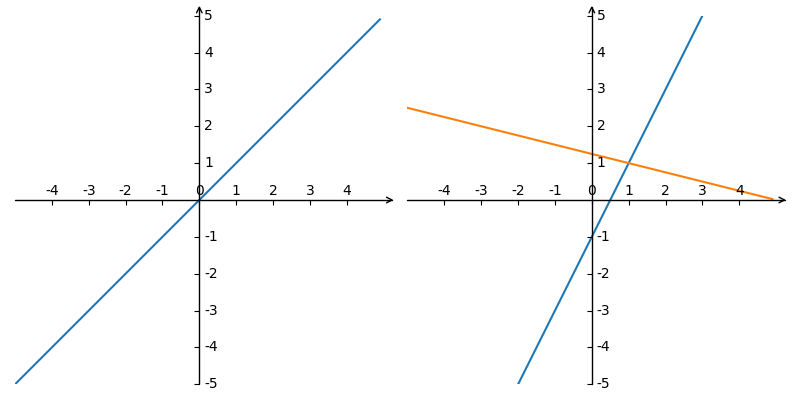
\includegraphics[height=4cm]{1.2-1.png}
\end{figure}

\begin{tcolorbox}
本题考察集合的概念和集合的描述方法。
\end{tcolorbox}






\newpage
\section{集合的基本运算}

本节要点:
\begin{itemize}
    \item 熟练掌握集合的运算法则。
\end{itemize}

~

集合的运算并没有什么难度。教材介绍了3中运算,交并补,我们可以做如下精确的定义。

\begin{definition}[集合的运算]
设三个集合$A,B,C$,若$A$中的任一元素同时属于$C$,且$B$中的任一元素也同时属于$C$,则称{\bf $C$为$A,B$的并集},记作$A\cup B$,即:
\[
A\cup B:=\left\{ a \middle| a\in A\text{或}a\in B \right\}
\]
若$C$中的任一元素同时属于$A$和$B$,则称{\bf $C$为$A,B$的交集},记作$A\cap B$,即:
\[
A\cap B:=\left\{ a \middle| a\in A\text{且}a\in B \right\}
\]
若我们将$A$中的同时属于$B$的元素去除,得到的集合称为{\bf $A$和$B$的差},也称为{\bf $B$关于$A$的补集},记作$A\cap \bar{B}$,即:
\[
A\cap \bar{B}:=\left\{ a \middle| a\in A\text{且}a\notin B \right\}
\]
\end{definition}

\begin{figure}[h]
\centering
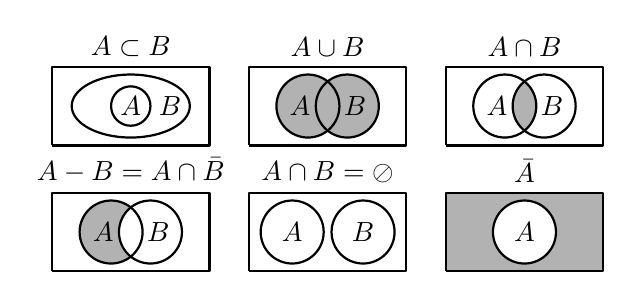
\begin{tikzpicture}[line join=round, scale=0.5]
% A in B
\coordinate (O) at (-5,1.6);
\draw[thick] ($(O)+(-2,-1)$)--($(O)+(2,-1)$)--($(O)+(2,1)$)--($(O)+(-2,1)$)--($(O)+(-2,-1)$);
\coordinate[label=above:{$A\subset B$}] (t) at ($($(O)+(-2,1)$)!0.5!($(O)+(2,1)$)$);
\draw[thick] ($(O)+(0,0)$) ellipse (1.5 and 0.8);
\draw[thick] ($(O)+(0,0)$) circle (0.5);
\coordinate[label=center:{$A$}] (a) at ($(O)+(0,0)$);
\coordinate[label=center:{$B$}] (b) at ($(O)+(1,0)$);
% A or B
\coordinate (O) at (0,1.6);
\draw[thick] ($(O)+(-2,-1)$)--($(O)+(2,-1)$)--($(O)+(2,1)$)--($(O)+(-2,1)$)--($(O)+(-2,-1)$);
\coordinate[label=above:{$A\cup B$}] (t) at ($($(O)+(-2,1)$)!0.5!($(O)+(2,1)$)$);
\fill[black!30!white] ($(O)+(-0.5,0)$) circle (0.8);
\fill[black!30!white] ($(O)+(0.5,0)$)  circle (0.8);
\draw[thick] ($(O)+(-0.5,0)$) circle (0.8);
\draw[thick] ($(O)+(0.5,0)$)  circle (0.8);
\coordinate[label=center:{$A$}] (a) at ($(O)+(-0.7,0)$);
\coordinate[label=center:{$B$}] (b) at ($(O)+(0.7,0)$);
% A and B
\coordinate (O) at (5,1.6);
\draw[thick] ($(O)+(-2,-1)$)--($(O)+(2,-1)$)--($(O)+(2,1)$)--($(O)+(-2,1)$)--($(O)+(-2,-1)$);
\coordinate[label=above:{$A\cap B$}] (t) at ($($(O)+(-2,1)$)!0.5!($(O)+(2,1)$)$);
\begin{scope}
\clip[draw] ($(O)+(-0.5,0)$) circle (0.8);
\fill[black!30!white] ($(O)+(0.5,0)$) circle (0.8);
\end{scope}
\draw[thick] ($(O)+(-0.5,0)$) circle (0.8);
\draw[thick] ($(O)+(0.5,0)$)  circle (0.8);
\coordinate[label=center:{$A$}] (a) at ($(O)+(-0.7,0)$);
\coordinate[label=center:{$B$}] (b) at ($(O)+(0.7,0)$);
% A - B
\coordinate (O) at (-5,-1.6);
\draw[thick] ($(O)+(-2,-1)$)--($(O)+(2,-1)$)--($(O)+(2,1)$)--($(O)+(-2,1)$)--($(O)+(-2,-1)$);
\coordinate[label=above:{$A-B=A\cap \bar{B}$}] (t) at ($($(O)+(-2,1)$)!0.5!($(O)+(2,1)$)$);
\fill[black!30!white] ($(O)+(-0.5,0)$) circle (0.8);
\draw[thick,fill=white] ($(O)+(0.5,0)$) circle (0.8);
\draw[thick] ($(O)+(-0.5,0)$) circle (0.8);
\coordinate[label=center:{$A$}] (a) at ($(O)+(-0.7,0)$);
\coordinate[label=center:{$B$}] (b) at ($(O)+(0.7,0)$);
% A and B is null
\coordinate (O) at (0,-1.6);
\draw[thick] ($(O)+(-2,-1)$)--($(O)+(2,-1)$)--($(O)+(2,1)$)--($(O)+(-2,1)$)--($(O)+(-2,-1)$);
\coordinate[label=above:{$A\cap B=\oslash $}] (t) at ($($(O)+(-2,1)$)!0.5!($(O)+(2,1)$)$);
\draw[thick] ($(O)+(-0.9,0)$) circle (0.8);
\draw[thick] ($(O)+(0.9,0)$)  circle (0.8);
\coordinate[label=center:{$A$}] (a) at ($(O)+(-0.9,0)$);
\coordinate[label=center:{$B$}] (b) at ($(O)+(0.9,0)$);
% not A
\coordinate (O) at (5,-1.6);
\fill[black!30!white] ($(O)+(-2,-1)$)--($(O)+(2,-1)$)--($(O)+(2,1)$)--($(O)+(-2,1)$)--cycle;
\draw[thick] ($(O)+(-2,-1)$)--($(O)+(2,-1)$)--($(O)+(2,1)$)--($(O)+(-2,1)$)--($(O)+(-2,-1)$);
\coordinate[label=above:{$\bar{A}$}] (t) at ($($(O)+(-2,1)$)!0.5!($(O)+(2,1)$)$);
\draw[thick,fill=white] ($(O)+(0,0)$) circle (0.8);
\coordinate[label=center:{$A$}] (a) at ($(O)+(0,0)$);
\end{tikzpicture}
\end{figure}

集合的运算除逻辑符号外,还可使用算术符号描述。

\begin{table}[h]
\centering
\begin{tabular}{ccc}
    \toprule
    运算 & 逻辑符号 & 算术符号\\
    \midrule
    并 & $A\cup B$ & $A+B$\\
    交 & $A\cap B$ & $AB$\\
    差 & $A\cap \bar{B}$ & $A-B$\\
    \bottomrule
\end{tabular}
\end{table}

\begin{tcolorbox}
集合的运算使得我们可以用一些简单集合的组合描述一个复杂集合。但要注意,这里的运算是逻辑运算,而非算术运算。
\end{tcolorbox}

集合的运算法则:
\begin{itemize}
    \item {\bf 交换律}:$AB=BA$
    \item {\bf 结合律}:$\left( A+B \right) +C=A+\left( B+C \right) ,\left( AB \right) C=A\left( BC \right) $
    \item {\bf 分配律}:$\left( A+B \right) C=\left( AC \right) +\left( AB \right) ,\left( AB \right) +C=\left( A+C \right) \left( B+C \right) $
    \item {\bf 德摩根律}:$\overline{A+B}=\bar{A}\bar{B},\overline{AB}=\bar{A}+\bar{B}$
\end{itemize}

~

其他常用运算公式:
\begin{align*}
& AB\subset A\subset A+B,\qquad AB\subset B\subset A+B \\
& AA=A \\
& A+A=A \\
& A+\bar{A}=\varOmega \\
& A-B=A\bar{B}=A-AB \\
& \left( A-B \right) +B=A+B
\end{align*}

\begin{tcolorbox}
上述运算法则和公式有些超纲,有兴趣可XML。
\end{tcolorbox}






\newpage
\section{充分条件和必要条件}

本节要点:
\begin{itemize}
    \item 了解命题的概念;
    \item 熟练掌握并深刻理解充分条件和必要条件的概念。
\end{itemize}

~

命题是一个陈述句,往往很简单,而且陈述是明确的、无歧义的,命题的结论要么为真、要么为假,只有其中一个结果,而且结果也是明确的、无歧义的。

对于充分条件和必要条件,下列四种说法等价:
\begin{itemize}
    \item 命题“若$p$,则$q$”为真命题;
    \item $p\Rightarrow q$;
    \item $p$是$q$的充分条件;
    \item $q$是$p$的必要条件。
\end{itemize}

\begin{tcolorbox}
对于命题、充分条件、必要条件,我们无需从形式逻辑方面完全掌握其概念,毕竟不是逻辑课程。我们只需了解它们是如何构建数学中的定义、定理、性质的。
\end{tcolorbox}

一般来讲,定义(definition)$D$是逻辑的起点,是一个人为的设定,不容置疑的。而判断一事物是否为$D$会比较复杂,定理(theorem)$T$给出了判断事物是否为$D$的简单方法,通常定理以充分条件的形式给出。一旦我们获得了一事物是$D$这个判断,那么该事物必然有$D$的性质(property)$P$,通常这类性质往往以必要条件的形式给出。
\[
T\rightarrow D\rightarrow P
\]

具体到解题中,已知条件通常以定理的前提给出,问题则以性质的结论要求计算或证明。所以,可以总结解题套路:
\begin{enumerate}
    \item 用定理将式子或图形框在某一定义中,如证明两个三角形相似即将两个三角形框在了相似这个定义中;
    \item 用性质得出结论,如计算另一个三角形的某个角。
\end{enumerate}
\[
\text{已知}\overset{T}{\Rightarrow}D\overset{P}{\Rightarrow}\text{结论}
\]

\begin{tcolorbox}
充要条件是整个高中乃至整个数学的思维范式!需要深刻领会。如何研究事物的运动规律?这是有一套固定的方法论的。数学上,我们不会单独讨论某个问题,而是将所有类似的问题总结提炼,形成定义、定理、性质。碰到具体问题,首先将问题转到数学空间,即归类到某个数学定义,然后用那个定义配套的定理和性质分析问题。这就是西方科学的基石,从亚里士多德开始的演绎法!
\end{tcolorbox}

\begin{tcolorbox}
演绎法是由一般到特殊的推理方法,与“归纳法”相对。最著名的演绎论恐怕莫过于:所有人都会死,苏格拉底是人,所以苏格拉底会死。演绎法中,“一般”是已知的事实,“特殊”是未知的结论。数学中,这个一般的已知的事实就是我们学习的各种数学概念、定理、公式,这个特殊就是各种题目。题目千千万万,但万变不离其宗,再抽象晦涩的题目总能化为最最基础的数学概念。事实上,高中数学也就是那么几个一个手数地过来的基础概念。
\end{tcolorbox}






\newpage
\section{全称量词和存在量词}

略。






\newpage
\section{本章小结}

形而上方面,本章介绍了数学的思维范式——演绎法,在以后的学习过程中需要不断加深认识。形而下方面,本章介绍了逻辑的基本知识。集合和逻辑用语是现代数学的语言基础。本章定义了一些数学符号,如$\cap ,\cup ,\in ,\forall ,\exists $,这些符号使得数学语言脱离了自然语言,去除了自然语言的模糊性,让数学更加清晰精准。随着学习的深入,我们会定义更多的数学符号,记住,数学符号就是为了精确、准确、无歧义地表述。

我们再用数学判断命题或计算某个值时,往往使用“定理—定义—性质”这个步骤。如计算下面$\bigtriangleup ABC$的角$\alpha $,我们可以按如下步骤:
\begin{enumerate}
    \item 用定理证明$\bigtriangleup ABC$和$\bigtriangleup abc$相似;
    \item 用性质得到$\alpha =60^\circ$。
\end{enumerate}

\begin{figure}[h]
\centering
\begin{minipage}{.49\textwidth}
\centering
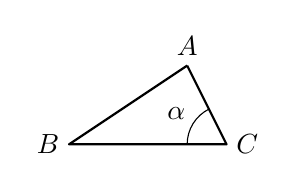
\begin{tikzpicture}[line join=round, scale=1]
\coordinate[label=above:{$A$}] (A) at (0.5,1);
\coordinate[label=left: {$B$}] (B) at (-1,0);
\coordinate[label=right:{$C$}] (C) at (1,0);
\draw[thick] (A)--(B)--(C)--(A);
\pic["$\alpha $",draw,angle radius=0.5cm,angle eccentricity=1.5] {angle=A--C--B};
\end{tikzpicture}
\end{minipage}
\begin{minipage}{.49\textwidth}
\centering
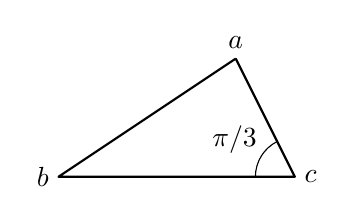
\begin{tikzpicture}[line join=round, scale=1.5]
\coordinate[label=above:{$a$}] (A) at (0.5,1);
\coordinate[label=left: {$b$}] (B) at (-1,0);
\coordinate[label=right:{$c$}] (C) at (1,0);
\draw[thick] (A)--(B)--(C)--(A);
\pic["$\pi /3$",draw,angle radius=0.5cm,angle eccentricity=1.8] {angle=A--C--B};
\end{tikzpicture}
\end{minipage}
\end{figure}

定义是逻辑起点,也是我们围绕的中心,是我们学习数学时的重中之重。定理是用来快速判断是否符合定义,让我们在逻辑上对定义有更深刻的认识。性质则是用来得到我们想要的结果。

~

\begin{example}[综合运用8,难度:$\star $]
已知
\begin{align*}
&A=\left\{ \left( x,y \right) \middle| 2x-y=0 \right\} \\
&B=\left\{ \left( x,y \right) \middle| 3x+y=0 \right\} \\
&C=\left\{ \left( x,y \right) \middle| 2x-y=3 \right\}
\end{align*}
求$A\cap B,A\cap C$,并解释它们的几何意义。
\end{example}

解:

\begin{align*}
&A\cap B=\left\{ \left( x,y \right) \middle| \left\{ \begin{array}{c}
	2x-y=0\\
	3x+y=0\\
\end{array} \right. \right\} \\
&A\cap C=\left\{ \left( x,y \right) \middle| \left\{ \begin{array}{c}
	2x-y=0\\
	2x-y=3\\
\end{array} \right. \right\}
\end{align*}

$A,B,C$几何上均表示平面的直线,$A\cap B$表示点即在直线$A$上也在直线$B$上,所以是它们的交点。不难发现,$A\cap B$是有交点的,但$A\cap C$表示两条平行线,没有交点。
\begin{figure}[ht]
\centering
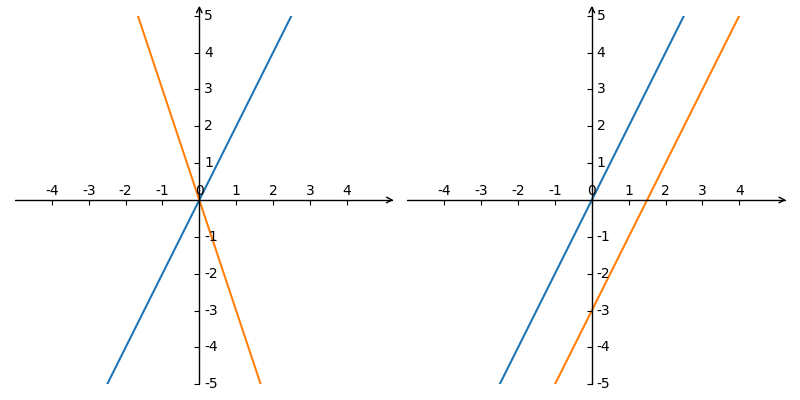
\includegraphics[height=4cm]{1.6-2.png}
\end{figure}

\begin{tcolorbox}
该题注意数形结合。
\end{tcolorbox}

~

\begin{example}[拓广探索12(2),难度:$\star \star \star $]
如图,在$\bigtriangleup ABC$中,$AD,BE,CF$分别为边$BC,AC,AB$上的高,证明$AD,BE,CF$交于点$O$。
\end{example}

解一,使用替换概念的思路:

在中学平面几何里面,我们学到过三角形有4个心:
\begin{itemize}
    \item 垂心,三角形三条高的交点;
    \item 重心,三角形三条中线的交点;
    \item 外心,三角形三条边的中垂线的交点,也是三角形外接圆的圆心;
    \item 内心,三角形三条角平分线的交点,也是三角形内切圆的圆心。
\end{itemize}
显然,在这里面最接近于三条高交点的是外心。于是,我们构建$\bigtriangleup A'B'C'$,使得$A'B'\parallel AB,A'C'\parallel AC,B'C'\parallel BC$。不难证明,$AD,BE,CF$为$\bigtriangleup A'B'C'$的中垂线,必交于一点,证毕。

\begin{figure}[h]
\centering
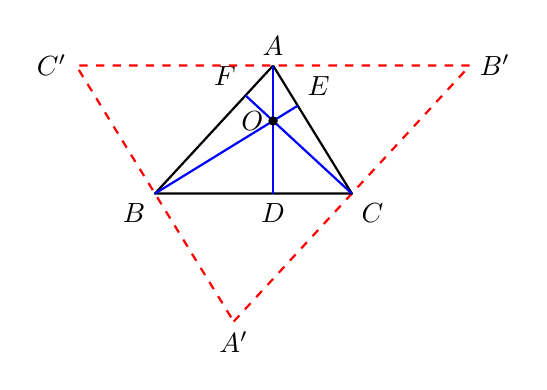
\begin{tikzpicture}[line join=round, scale=2.5]
\pgfmathparse{0.6/2.5}
\coordinate[label=left:       {$C'$}] (C') at (-1,0);
\coordinate[label=right:      {$B'$}] (B') at (1,0);
\coordinate[label=below:      {$A'$}] (A') at (-0.2,-1.3);
\coordinate[label=above:      {$A$}]  (A)  at ($(C')!0.5!(B')$);
\coordinate[label=below left: {$B$}]  (B)  at ($(C')!0.5!(A')$);
\coordinate[label=below right:{$C$}]  (C)  at ($(A')!0.5!(B')$);
\coordinate[label=below:      {$D$}]  (D)  at ($(B)!(A)!(C)$);
\coordinate[label=above right:{$E$}]  (E)  at ($(A)!(B)!(C)$);
\coordinate[label=above left: {$F$}]  (F)  at ($(A)!(C)!(B)$);
\draw[thick,dashed,red] (A')--(B')--(C')--(A');
\draw[thick] (A)--(B)--(C)--(A);
\draw[thick,blue,name path=l1] (A)--(D);
\draw[thick,blue,name path=l2] (B)--(E);
\draw[thick,blue] (C)--(F);
\path [name intersections={of=l1 and l2}] coordinate[label=left:$O$] (O) at (intersection-1);
\fill (O) circle (\pgfmathresult mm);
\end{tikzpicture}
\end{figure}

解二,使用替换命题的思路:

$AD$并不是垂线,只是过$O$的直线,交$BC$于$D$,证明$AD\bot BC$。

借用向量的知识,两个向量垂直等价于几何上的垂直,于是:
\begin{align*}
&\because \overrightarrow{BE}\cdot \overrightarrow{AC}=0\Rightarrow \overrightarrow{BO}\cdot \overrightarrow{AC}=0 \\
&\therefore \left( \overrightarrow{AO}-\overrightarrow{AB} \right) \cdot \overrightarrow{AC}=0 \\
&\therefore \overrightarrow{AO}\cdot \overrightarrow{AC}=\overrightarrow{AB}\cdot \overrightarrow{AC}
\end{align*}
同理:
\[
\overrightarrow{AO}\cdot \overrightarrow{AB}=\overrightarrow{AC}\cdot \overrightarrow{AB}
\]
于是:
\begin{align*}
&\because \overrightarrow{AO}\cdot \overrightarrow{AC}=\overrightarrow{AO}\cdot \overrightarrow{AB}\Rightarrow \overrightarrow{AO}\cdot \left( \overrightarrow{AC}-\overrightarrow{AB} \right) =0 \\
&\therefore \overrightarrow{AO}\cdot \overrightarrow{BC}=0
\end{align*}

\begin{tcolorbox}
解法一属于偷换概念,也是一种不错的技巧。解法二属于数形结合,用代数的方法解几何问题。
\end{tcolorbox}










\chapter{不等式}

本章讨论不等式。不等式常用于讨论函数最大值最小值,在工程实践中也有现实意义。

本章要点:
\begin{itemize}
    \item 不等式的性质。
    \item 四类均值及其不等式。
    \item 基本不等式和二次函数。
\end{itemize}

\newpage
\section{等式性质与不等式性质}

本节要点:
\begin{itemize}
    \item 熟练掌握等式的性质;
    \item 熟练掌握不等式的性质。
\end{itemize}

~

若$a,b,c\in \mathbb{R} $,则有等式的性质:
\begin{itemize}
    \item 性质1:$a=b\Rightarrow b=a$;
    \item 性质2:$a=b,b=c\Rightarrow a=c$;
    \item 性质3:$a=b\Rightarrow a\pm c=b\pm c$;
    \item 性质4:$a=b\Rightarrow ac=bc$;
    \item 性质5:$a=b,c\ne 0\Rightarrow a/c=b/c$。
\end{itemize}

\begin{tcolorbox}
性质1表示了对等性,性质2表示了传递性,性质3表示了加减不变性,性质4、5表示了乘除的不变性。
\end{tcolorbox}

根据算术运算的法则,不难得出不等式的性质,若$a,b,c\in \mathbb{R} $,则有不等式的性质:
\begin{itemize}
    \item 性质1:$a>b\Leftrightarrow b<a$;
    \item 性质2:$a>b,b>c\Rightarrow a>c$;
    \item 性质3:$a>b\Rightarrow a\pm c>b\pm c$;
    \item 性质4:$a>b,c>0\Rightarrow ac>bc$,$a>b,c<0\Rightarrow ac<bc$;
    \item 性质5:$a>b,c>d\Rightarrow a+c>b+d$;
    \item 性质6:$a>b>0,c>d>0\Rightarrow ac>bd$;
    \item 性质7:$a>b>0\Rightarrow a^n>b^n,n\in \mathbb{N} \text{且}n>0$。
\end{itemize}

~

等式和不等式的性质本身并无难度,关键掌握两个点。

首先,不等式在代数中表示一个约束,通常多个约束是逻辑与的关系,除非特别指明逻辑或,所以如下的三种表示方法是等价的:
\begin{align*}
&A<B,A>C \\
&C<A<B \\
&\left\{ \begin{array}{c}
	A<B\\
	A>C\\
\end{array} \right.
\end{align*}

其次,在判断两个式子的不等关系时,常用的方法是相减后和0比大小。当然也可以相除后和$\pm 1$比大小,但高中阶段不常用。

~

\begin{example}[拓广探索12,难度:$\star \star \star \star $]
火车站有某公司待运的甲种货物1530t,乙种货物1150t,现计划用A、B两种型号的货厢共50节运送这批货物。已知35t甲种货物和15t乙种货物可装满一节A型货厢,25t甲种货物和35t乙种货物可装满一节B型货厢,据此安排A、B两种货厢的节数,共有几种方案?若每节A型货厢的运费是0.5万元,每节B型货厢的运费是0.8万元,哪种方案的运费较少?
\end{example}

解:

设两种型号货厢各$A,B$个,不难得到如下4个约束:
\begin{itemize}
    \item 共运载甲种货物不少于1530t,$35A+25B\geqslant 1530$;
    \item 共运载乙种货物不少于1150t,$15A+35B\geqslant 1150$;
    \item 两种货厢共不多于50节,$A+B\leqslant 50$;
    \item 货厢为自然数,$A,B\in \mathbb{N} $。
\end{itemize}
取$A$为横坐标,$B$为从坐标,图形如下:
\begin{figure}[h]
\centering
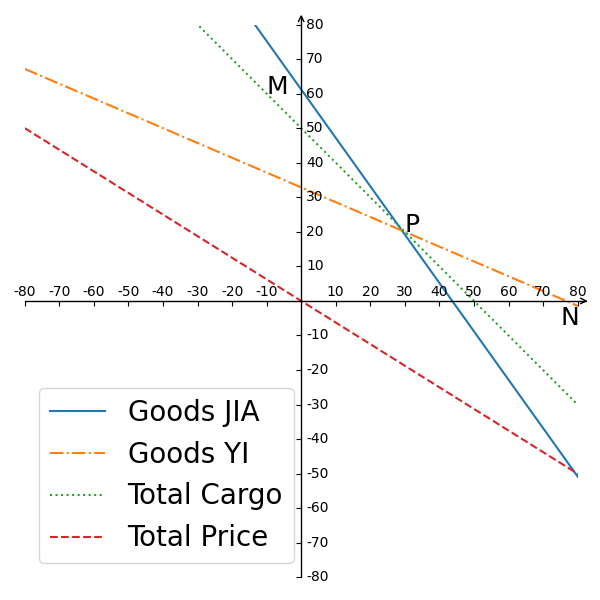
\includegraphics[height=8cm]{2.1-1.png}
\end{figure}

反映到图象上,即要求:
\begin{itemize}
    \item 共运载甲种货物不少于1530t,在蓝实线的上方;
    \item 共运载乙种货物不少于1150t,在橙点划线的上方;
    \item 两种货厢共不多于50节,在绿虚线的下方。
\end{itemize}
图中很小的一个范围。

求解:
\begin{align*}
&\because \begin{cases}
	35A+25B\geqslant 1530\\
	15A+35B\geqslant 1150\\
\end{cases} \\
&\therefore 50A+60B\geqslant 2680\Rightarrow B\geqslant \frac{2680-50A}{60} \\
&\because A+B\leqslant 50\Rightarrow B\leqslant 50-A \\
&\therefore \frac{2680-50A}{60}\leqslant 50-A \\
&\therefore A\leqslant 32
\end{align*}
$A$从32往下取自然数,的最终结果如下表:
\begin{table}[h]
\centering
\begin{tabular}{cccccc}
    \toprule
     & A型货厢 & B型货厢 & 甲种货物 & 乙种货物 & 运费\\
    \midrule
    方案一 & 30 & 20 & 1550 & 1150 & 31\\
    方案二 & 29 & 21 & 1540 & 1170 & 31.3\\
    方案三 & 28 & 22 & 1530 & 1190 & 31.6\\
    \bottomrule
\end{tabular}
\end{table}

\begin{tcolorbox}
本题很抽象,关键在于如何将生活问题转换为数学问题,即根据要求列出4个约束关系,一旦得到了这4个不等式,就完成了关键一步,余下的就是求解不等式而已。在求解不等式方面,本题只涉及一次不等式,还是很简单的。
\end{tcolorbox}






\newpage
\section{基本不等式}

本节要点:
\begin{itemize}
    \item 掌握四类均值的概念;
    \item 深刻理解四类均值的实际意义;
    \item 深刻理解围绕它们的不等式。
\end{itemize}

~

教材只讨论了一个基本不等式
\[
a+b\geqslant 2\sqrt{ab}
\]
但我们进行扩展。

\begin{definition}
设实数$x_1,x_2,\cdots ,x_n\in \mathbb{R} $,称:
\begin{itemize}
    \item 它们的和与个数的比为{\bf 算数均值}(arithmetic mean),记作$A_n$;
    \item 它们各自的倒数的算数均值的倒数为{\bf 调和均值}(harmonic mean),也成为{\bf 倒数均值},记作$H_n$;
    \item 它们各自的平方的算数均值的算数平方根为{\bf 平方均值}(quadratic mean),也称为{\bf 均方根}(Root Mean Square,RMS),记作$Q_n$;
    \item 它们的乘积的$n$次算数平方根为{\bf 几何均值}(geometric mean),记作$G_n$。
\end{itemize}
\begin{align*}
&A_n=\frac{x_1+x_2+\cdots +x_n}{n}=\frac{\sum_{i=i}^n{x_i}}{n} \\
&H_n=\frac{n}{\frac{1}{x_1}+\frac{1}{x2}+\cdots \frac{1}{x_n}}=\frac{n}{\sum_{i=i}^n{\frac{1}{x_i}}} \\
&Q_n=\sqrt{\frac{x_{1}^{2}+x_{2}^{2}+\cdots +x_{n}^{2}}{n}}=\sqrt{\frac{\sum_{i=i}^n{x_{i}^{2}}}{n}} \\
&G_n=\sqrt[n]{x_1x_2\cdots x_n}
\end{align*}
\end{definition}

各类均值的产生是有其生产实践的背景的,目的是在一个目标总量下用均值代替各个分量,也即:
\[
\text{均值的和}=\text{各分量的和}=\text{目标总量}
\]

{\bf 算术均值}

算数均值非常直观,其目标总量就是直接累加,如平均成绩、平均每个人分到的苹果数等。

{\bf 调和均值}

调和均值的目标总量是倒数和,换个表述方式或许更易理解:
\[
\frac{1}{x_1}+\frac{1}{x_2}+\cdots \frac{1}{x_n}=\frac{n}{H_n}
\]
往往用于计算某些“率”,如已知并联电阻$R_1,R_2$求等效电阻,这里的目标总量就是流过两个支路的电流总和:
\[
\frac{U}{R_e}=\frac{U}{R_1}+\frac{U}{R_2} \quad \Rightarrow \quad \frac{1}{R_e}=\frac{1}{R_1}+\frac{1}{R_2}
\]
还如平均速度等,可自行推导。

{\bf 平方均值}

平方均值的目标总量在平方和,往往是跟能量相关,常用于计算交流电的平均电压、平均电流等。如为表征正弦电压的做功能力,我们可以定义电压的有效值为该周期性电压在电阻上一个周期内所作的相同的功,目标总量为总做功,即:
\[
\int_0^T{\frac{u^2\left( t \right)}{R}\cdot dt}=\frac{U^2}{R}\cdot T \quad \Rightarrow \quad U=\sqrt{\frac{1}{T}\cdot \int_0^T{\frac{u^2\left( t \right)}{R}\cdot dt}}
\]

{\bf 几何均值}

几何均值的目标总量为几何体的测度,如平面的面积、三维物体的体积,我们用等面积的正方形等效长方形,用等体积的正方体等效长方体等。

\begin{figure}[h]
\centering
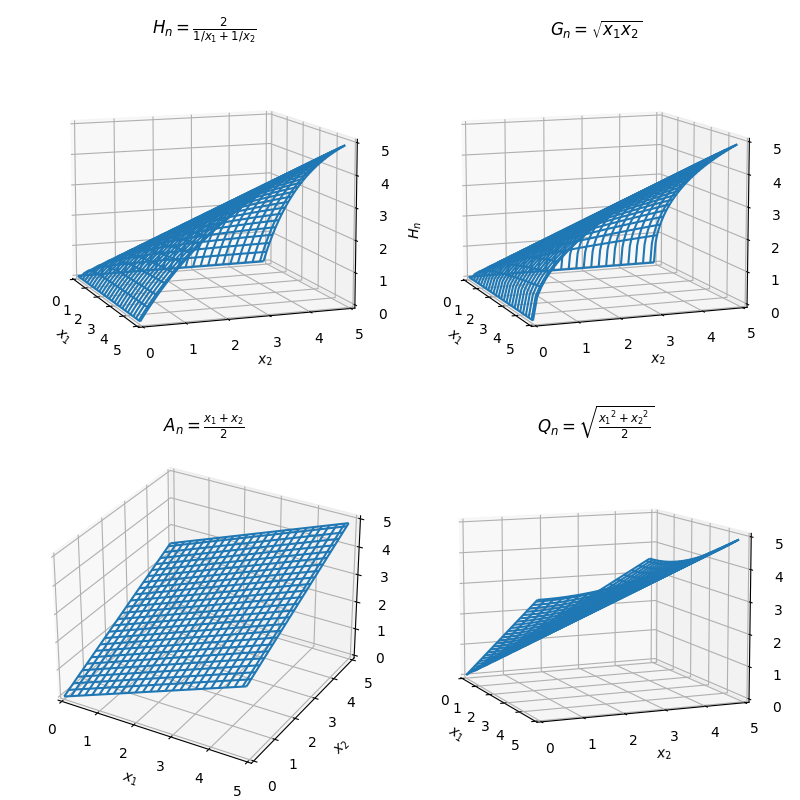
\includegraphics[height=9cm]{2.2-1.png}
\end{figure}

四类均值的图形如上,为方便作图我们只取两个变量,不难发现:
\begin{itemize}
    \item $H_n$和$G_n$弯向下,且$H_n$的下弯速度大于$G_n$;
    \item $A_n$是一个平面,必然大于$H_n$和$G_n$;
    \item $Q_n$弯向上,必然大于$A_n$;
    \item $x_1=x_2$为它们公共的交线。
\end{itemize}

\begin{theorem}[均值不等式定理]
设实数$x_1,x_2,\cdots ,x_n\in \mathbb{R} $,则四类均值有:
\[
H_n\leqslant G_n\leqslant A_n\leqslant Q_n
\]
或写成:
\[
\frac{n}{\sum_{i=i}^n{\frac{1}{x_i}}}\leqslant \sqrt[n]{x_1x_2\cdots x_n}\leqslant \frac{\sum_{i=i}^n{x_i}}{n}\leqslant \sqrt{\frac{\sum_{i=i}^n{x_{i}^{2}}}{n}}
\]
当且仅当$x_1=x_2=\cdots =x_n$时等号成立。
\end{theorem}

\begin{proof}
构造直角三角形$\bigtriangleup ABC$,如图,令$AB=\frac{x_1+x_2}{2},AC=\frac{x_1-x_2}{2}$,由勾股定理可得$BC=\sqrt{\frac{{x_1}^2+{x_2}^2}{2}}$,可见:
\[
\frac{x_1+x_2}{2}\leqslant \sqrt{\frac{{x_1}^2+{x_2}^2}{2}}
\]

\begin{figure}[h]
\centering
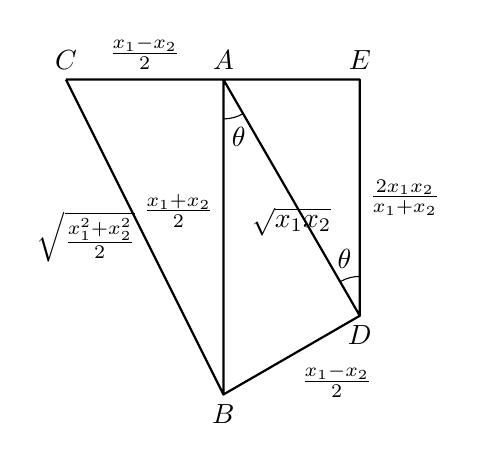
\begin{tikzpicture}[line join=round, scale=1]
\coordinate[label=above:{$A$}] (A) at (0,0);
\coordinate[label=above:{$C$}] (C) at (-2,0);
\coordinate[label=below:{$B$}] (B) at (0,-4);
\coordinate[label=above:{$E$}] (E) at (1.732,0);
\coordinate[label=below:{$D$}] (D) at (1.732,-3);
\coordinate[label=above:      {$\frac{x_1-x_2}{2}$}]                    (ac) at ($(A)!0.5!(C)$);
\coordinate[label=left:       {$\sqrt{\frac{x_{1}^{2}+x_{2}^{2}}{2}}$}] (bc) at ($(C)!0.5!(B)$);
\coordinate[label=above left: {$\frac{x_1+x_2}{2}$}]                    (ab) at ($(A)!0.5!(B)$);
\coordinate[label=below:      {$\sqrt{x_1x_2}$}]                        (ad) at ($(A)!0.5!(D)$);
\coordinate[label=below right:{$\frac{x_1-x_2}{2}$}]                    (bd) at ($(B)!0.5!(D)$);
\coordinate[label=right:      {$\frac{2x_1x_2}{x_1+x_2}$}]              (de) at ($(D)!0.5!(E)$);
\draw[thick] (C)--(E)--(D)--(B)--(C) (B)--(A)--(D);
\pic["$\theta $",draw,angle radius=0.5cm,angle eccentricity=1.5] {angle=B--A--D};
\pic["$\theta $",draw,angle radius=0.5cm,angle eccentricity=1.5] {angle=E--D--A};
\end{tikzpicture}
\end{figure}

再以$AB$为斜边构造直角三角形$\bigtriangleup ABD$,令$BD=AC=\frac{x_1-x_2}{2}$,由勾股定理可得$AD=\sqrt{x_1x_2}$,可见:
\[
\sqrt{x_1x_2}\leqslant \frac{x_1+x_2}{2}
\]

继续作直角三角形$\bigtriangleup ADE$,令$ED\parallel AB$,于是$\angle BAD=\angle ADE=\theta $,则有:
\begin{align*}
&\because \cos \theta =\frac{AD}{AB}=\frac{ED}{AD} \\
&\therefore ED=\frac{AD^2}{AB}=\frac{x_1x_2}{\frac{x_1+x_2}{2}}=\frac{2x_1x_2}{x_1+x_2}=\frac{2}{\frac{1}{x_1}+\frac{1}{x_2}} \\
&\therefore \frac{2}{\frac{1}{x_1}+\frac{1}{x_2}}\leqslant \sqrt{x_1x_2}
\end{align*}
\end{proof}

\begin{proof}
使用向量的方法证明
\[
\frac{x_1+x_2}{2}\leqslant \sqrt{\frac{{x_1}^2+{x_2}^2}{2}}
\]
化简如下:
\[
\frac{x_1\cdot \frac{\sqrt{2}}{2}+x_2\cdot \frac{\sqrt{2}}{2}}{\sqrt{{x_1}^2+{x_2}^2}}\leqslant 1
\]
于是就可以发现,分子是两个向量的内积,分母是向量的模,整个表达式就是两个向量夹角的余弦,于是可设$\boldsymbol{a}=\left( x_1,x_2 \right) ,\boldsymbol{b}=\left( \frac{\sqrt{2}}{2},\frac{\sqrt{2}}{2} \right) $,得到:
\[
\cos \theta =\frac{\boldsymbol{a}\cdot \boldsymbol{b}}{\left| \boldsymbol{a} \right|\left| \boldsymbol{b} \right|}=\frac{x_1\cdot \frac{\sqrt{2}}{2}+x_2\cdot \frac{\sqrt{2}}{2}}{\sqrt{{x_1}^2+{x_2}^2}}\leqslant 1
\]
\end{proof}

~

\begin{example}[综合运用4,难度:$\star $]
已知$x,y,z$都是整数,求证
\[
\left( x+y \right) \left( y+z \right) \left( z+x \right) \geqslant 8xyz
\]
\end{example}

解:

\begin{align*}
&\quad \left( x+y \right) \left( y+z \right) \left( z+x \right) \\
&=\left( xy+xz+y^2+yz \right) \left( z+x \right) \\
&=xyz+x^2y+xz^2+x^2z+y^2z+y^2x+yz^2+xyz
\end{align*}
观察分析:
\begin{align*}
&x^2y+yz^2\geqslant 2y\sqrt{x^2z^2}=2xyz \\
&xz^2+y^2x\geqslant 2x\sqrt{z^2y^2}=2xyz \\
&x^2z+y^2z\geqslant 2z\sqrt{x^2y^2}=2xyz
\end{align*}
略,证毕。

\begin{tcolorbox}
本题只需尝试将左边展开即可发现方法。
\end{tcolorbox}

~

\begin{example}[拓广探索7,难度:$\star \star $]
一家商店使用一架两臂不等长的天平秤黄金,一位顾客到商店购买10g黄金,售货员先将5g的砝码放在天平左盘中,取出一些黄金放在天平右盘中使天平平衡;再将5g的砝码放在天平的右盘中,再取出一些黄金放在天平左盘中使天平平衡;最后将两次称得的黄金交给顾客。你认为顾客购得的黄金是小于10g,等于10g,还是大于10g?为什么?
\end{example}

解:

这个问题较为复杂,我们可以先尝试用一些数学式子描述该问题。假设天平左右两个臂的臂长分别为$l_L,l_R$,则根据力矩相等易得两次称重黄金的数学表示为:
\begin{align*}
&5\cdot l_L=A\cdot l_R \\
&B\cdot l_L=5\cdot l_R
\end{align*}
稍稍化简得:
\begin{align*}
&A=5\cdot \frac{l_L}{l_R} \\
&B=5\cdot \frac{l_R}{l_L}
\end{align*}
易得:
\[
A+B\geqslant 2\sqrt{5\cdot \frac{l_L}{l_R}\cdot 5\cdot \frac{l_R}{l_L}}=10
\]

\begin{tcolorbox}
本题关键在于获得$A,B$的表达式,一旦获得了,不难发现其互为倒数的关系,也就能自然想到基本不等式了。
\end{tcolorbox}

~

\begin{example}[拓广探索8,难度:$\star \star $]
设矩形$ABCD$($AB>AD$)的周长为24cm,把$\bigtriangleup ABC$沿$AC$向$\bigtriangleup ADC$折叠,$AB$折过去后交$DC$于点$P$。
设$AB=x\mathrm{cm}$,求$\bigtriangleup ADP$的最大面积及相应$x$的值。
\end{example}

\begin{figure}[h]
\centering
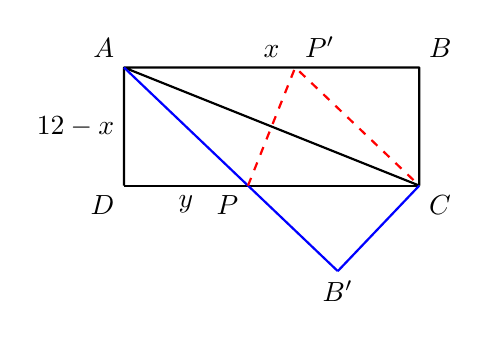
\begin{tikzpicture}[line join=round, scale=0.75]
\coordinate[label=above left: {$A$}]  (A)  at (-2.5,1);
\coordinate[label=above right:{$B$}]  (B)  at (2.5,1);
\coordinate[label=below right:{$C$}]  (C)  at (2.5,-1);
\coordinate[label=below left: {$D$}]  (D)  at (-2.5,-1);
\draw[thick] (D)--(A)--(B)--(C) (A)--(C);
\coordinate                     (tb) at ($(A)!(B)!(C)$);
\coordinate[label=below:{$B'$}] (B') at ($(B)!2.0!(tb)$);
\draw[thick,name path=l1] (D)--(C);
\draw[thick,blue,name path=l2] (A)--(B');
\path [name intersections={of=l1 and l2}] coordinate[label=below left:$P$] (P) at (intersection-1);
\draw[thick,blue] (B')--(C);
\coordinate                           (tp) at ($(A)!(P)!(C)$);
\coordinate[label=above right:{$P'$}] (P') at ($(P)!2.0!(tp)$);
\draw[thick,dashed,red] (P)--(P')--(C);
\coordinate[label=above:{$x$}]    (x)  at ($(A)!0.5!(B)$);
\coordinate[label=left: {$12-x$}] (x') at ($(A)!0.5!(D)$);
\coordinate[label=below:{$y$}]    (y)  at ($(D)!0.5!(P)$);
\end{tikzpicture}
\end{figure}

解:

令$DP$长$y$,则$\bigtriangleup ADP$的面积为:
\[
S_{\bigtriangleup ADP}=\frac{1}{2}\left( 12-x \right) y
\]
不难证明$\bigtriangleup ADP,\bigtriangleup CB'P$均为直角三角形,且全等,于是
\begin{align*}
&\because PC=PA=\sqrt{\left( 12-x \right) ^2+y^2} \\
&\therefore x=\sqrt{\left( 12-x \right) ^2+y^2}+y \\
&\therefore y=\frac{12x-72}{x}
\end{align*}
带入面积消去$y$,得:
\begin{align*}
S_{\bigtriangleup ADP}&=\frac{1}{2}\left( 12-x \right) y=\frac{1}{2}\left( 12-x \right) \frac{12x-72}{x} \\
&=6\cdot \frac{-x^2+18x-72}{x} \\
&=6\cdot \left( -x-\frac{72}{x}+18 \right)
\end{align*}
其中,$x+\frac{72}{x}\geqslant 2\sqrt{72}=12\sqrt{2}$,当且仅当$x=\frac{72}{x},x=\sqrt{72}$时等号成立,于是:
\[
S_{\bigtriangleup ADP}\leqslant 6\cdot \left( 18-12\sqrt{2} \right)
\]

\begin{tcolorbox}
本题的关键在于获得$S_{\bigtriangleup ADP}$的表达式和$x,y$的约束关系。一旦获得了,接下去就是化简和基本不等式。
\end{tcolorbox}

\begin{tcolorbox}
高中阶段的求解最值问题,最终都会转化为求解
\[
\left( Ax \right) +\left( \frac{B}{x} \right) \quad \text{或} \quad \left( Ax \right) \cdot \left( \frac{B}{x} \right)
\]
的最值问题,也即基本不等式。关键在于理解问题和观察图形,将实际问题或几何图形建模成代数问题。上面两题很有典型性,一题是实际应用题,另一题是几何题。结合上一章的说到的数学范式,认真思考上面两题,总结你的解题范式,XML。
\end{tcolorbox}






\newpage
\section{二次函数与一元二次方程、不等式}

本节要点:
\begin{itemize}
    \item 从基本不等式深刻理解二次函数的最值。
\end{itemize}

~

虽然二次函数的标准形式为$y=ax^2+bx+c$,但以下方式更能说明二次函数:
\[
y=a\left( x+b \right) ^2+c
\]
\begin{itemize}
    \item 首先,通过$a$变换开口大小和方向,$a$越小开口越宽大,$a>0$开口向上;
    \item 然后,通过$b$进行沿{\it x}轴的平移,$b>0$左移;
    \item 最后,通过$c$进行沿{\it y}轴的平移,$c>0$上移。
\end{itemize}

\begin{figure}[h]
\centering
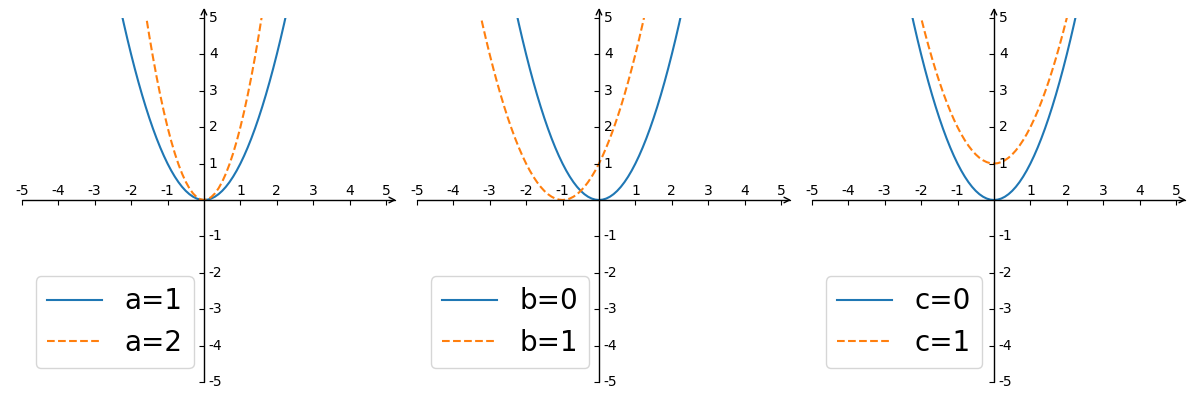
\includegraphics[height=4cm]{2.3-1.png}
\end{figure}

二次函数和基本不等式也可以相互推导。设某个变量$y$由$x,z$乘积决定,而$x,z$有关系$x+z=c$,其中 $c$为常数,于是:
\[
\begin{cases}
	y=x\cdot z\\
	x+z=c\\
\end{cases}\Rightarrow y=x\cdot \left( c-x \right)
\]
由基本不等式可得:
\[
y=x\cdot \left( c-x \right) \leqslant \left[ \frac{x+\left( c-x \right)}{2} \right] ^2=\frac{c^2}{4}
\]
用二次函数的方法:
\[
y=-x^2+cx
\]
当且仅当$x=\frac{c}{2}$时,$y$取最大值$y_{\max}=\frac{c^2}{4}$。

\begin{tcolorbox}
当两个变量的和为常量时,它们的积有最大值,这点从基本不等式和二次函数都能得到一样的结果。
\end{tcolorbox}

\begin{tcolorbox}
工程中,我们通常为最值构造一个二次函数$y=f\left( x_1,x_2 \right) $,用$ax_1+bx_2=c$作为两个变量的约束条件,得到一个二次函数,最终可求解最值。
\end{tcolorbox}

~

\begin{example}[综合运用4,难度:$\star $]
一名同学以初速度$v_0=12\mathrm{m}/\mathrm{s}$竖直向上抛一排球,排球能够在抛出点2m以上大的位置最多停留多长时间(精确到0.01s)?
\end{example}

\begin{figure}[h]
\centering
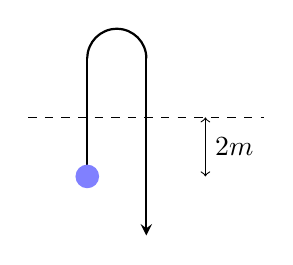
\begin{tikzpicture}[line join=round, scale=0.75]
\draw[thick] (0,0)--(0,2);
\draw[thick] (1,2) arc [start angle=0,end angle=180,radius=0.5cm];
\draw[thick,-stealth] (1,2)--(1,-1);
\fill[blue!50!white] (0,0) circle (2mm);
\draw[dashed] (-1,1)--(3,1);
\draw[<->] (2,1)--(2,0);
\coordinate[label=right:{$2m$}] (t) at (2,0.5);
\end{tikzpicture}
\end{figure}

解:

排球距抛出点高度和时间的关系如下:
\[
h=v_0t-\frac{1}{2}gt^2
\]
带入$v_0=12\mathrm{m}/\mathrm{s},g=10\mathrm{m}/\mathrm{s}^2,h\geqslant 2\mathrm{m}$得:
\[
12t-5t^2\geqslant 2
\]
令$5t^2-12t+2=0$,解得$t_{1,2}=\frac{12\pm \sqrt{12^2-4\cdot 5\cdot 2}}{2\cdot 5}=2.220 \,\, \mathrm{or} \,\, 0.180$,于是停留时间为$t=2.220-0.180=2.04\mathrm{s}$。

\begin{tcolorbox}
本题看似难,其实一点不难,物理问题已经转化为数学问题,剩下的就是体力活。
\end{tcolorbox}






\newpage
\section{扩展知识:\texorpdfstring{$y=x+\frac{1}{x}$}{y=x+1/x}的图形}

本节我们绘制
\[
y=ax+\frac{b}{x}
\]
的图形,以加深对基本不等式的理解。

~

由于函数是奇函数,且$x\ne 0$,所以我们只绘制$x>0$部分,先从最基本的开始,如下函数:
\[
y=x+\frac{1}{x} \qquad x>0
\]
图形如下,不难发现:
\begin{itemize}
    \item 图形由两部分组成,左边是$\frac{1}{x}$主导,右边是$x$主导;
    \item $y$先减小后增大,当$x=1$时取最小值2;
    \item $x=0$和$y=x$是函数的两条渐近线。
\end{itemize}

\begin{figure}[h]
\centering
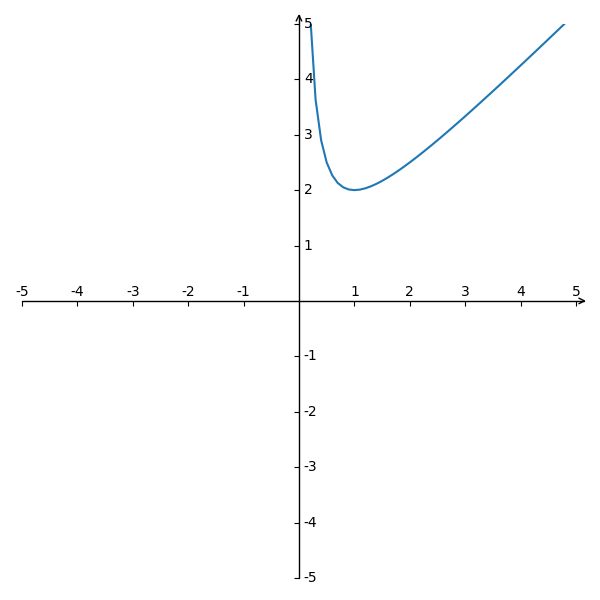
\includegraphics[height=6cm]{2.4-1.png}
\end{figure}

~

若我们调整$a$
\begin{align*}
&y=0.5x+\frac{1}{x} \\
&y=x+\frac{1}{x} \\
&y=2x+\frac{1}{x}
\end{align*}
则函数图形如下。

\begin{figure}[ht]
\centering
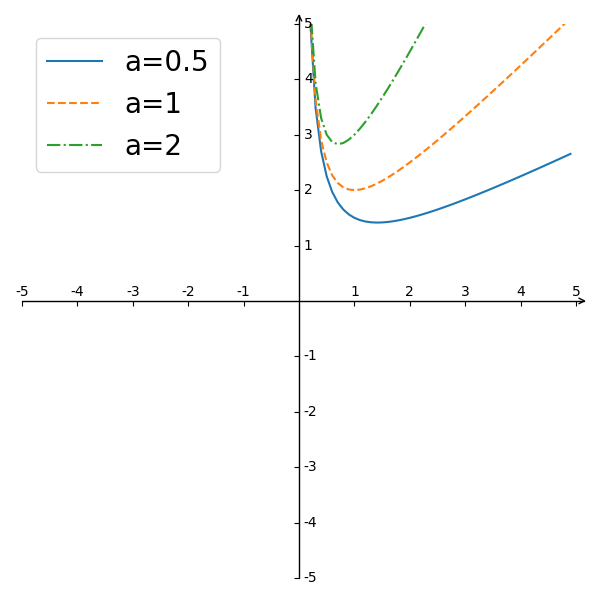
\includegraphics[height=6cm]{2.4-2.png}
\end{figure}

~

若我们调整$b$
\begin{align*}
&y=x+\frac{0.5}{x} \\
&y=x+\frac{1}{x} \\
&y=x+\frac{2}{x}
\end{align*}
则函数图形如下。

\begin{figure}[h]
\centering
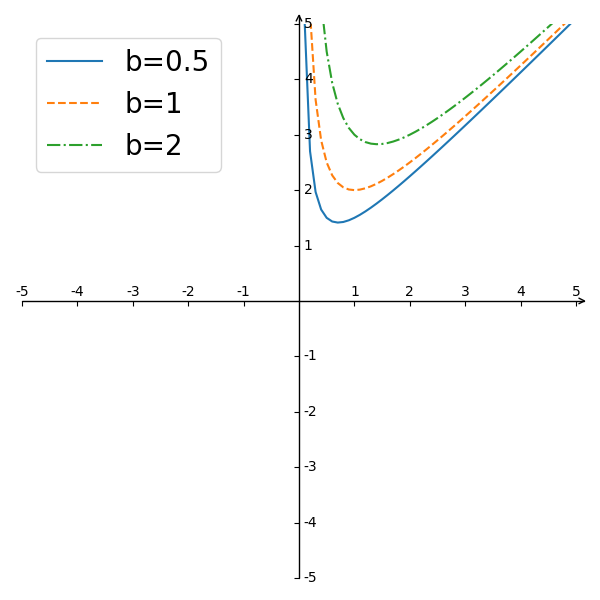
\includegraphics[height=6cm]{2.4-3.png}
\end{figure}

不难发现:
\begin{itemize}
    \item 调节$a$,影响的是$x$部分,图象上反映在右侧变化较大;
    \item 调节$b$,影响的是$1/x$部分,图象上反映在左侧变化较大;
    \item 无论调节$a$还是$b$,最值都会发生变化。
\end{itemize}






\newpage
\section{本章小结}

本章讨论了不等式,特别讨论了基本不等式和二次函数的最值。

特别要注意四类均值及其关系:
\[
\frac{n}{\sum_{i=i}^n{\frac{1}{x_i}}}\leqslant \sqrt[n]{x_1x_2\cdots x_n}\leqslant \frac{\sum_{i=i}^n{x_i}}{n}\leqslant \sqrt{\frac{\sum_{i=i}^n{x_{i}^{2}}}{n}}
\]
即:
\[
\text{调和}\leqslant \text{几何}\leqslant \text{算数}\leqslant \text{平方}
\]

其次要将基本不等式和二次函数的最值两者融会贯通,通过基本不等式分析二次函数最值的由来。

~

\begin{example}[综合运用5,难度:$\star $]
若$a,b>0$,且$ab=a+b+3$,求$ab$的取值范围。
\end{example}

解一:

题意为求函数$y=ab$的取值范围,且$a,b$有约束$ab=a+b+3$。将约束化简得:
\[
a=\frac{b+3}{b-1} \qquad b>1
\]
带入函数得到:
\[
y=ab=b\cdot \frac{b+3}{b-1} \qquad b>1
\]
不是很明显,但有$x\cdot \frac{1}{x}$的形式,化简该函数:
\begin{align*}
y=b\cdot \frac{b-1+4}{b-1}=\frac{4b}{b-1}+b=\frac{4b-4+4}{b-1}+b=\frac{4}{b-1}+\left( b-1 \right) +5
\end{align*}
易得$\left( b-1 \right) ^2=4$即$b=3$时,$y$有最小值$y_{\min}=9$,函数图象如下。
\begin{figure}[h]
\centering
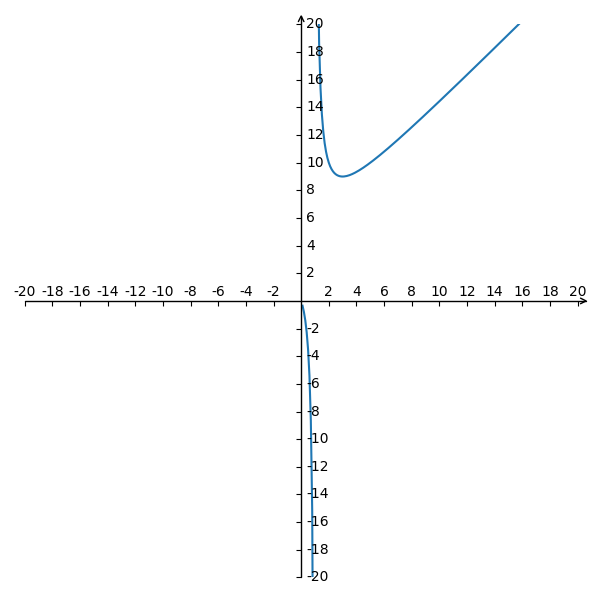
\includegraphics[height=5cm]{2.5-1.png}
\end{figure}

这里,我们将$b\in \left( 0,1 \right) $部分绘制出来,但是由于$a>$的限制,实际$b$的取值范围为$\left( 1,+\infty \right) $。

解二:

观察约束条件和要求的取值函数,$a,b$对称,所以可以直接考察约束条件:
\[
ab=a+b+3\geqslant 2\sqrt{ab}+3
\]
当且仅当$a=b$时成立。于是,可令$y=\sqrt{ab}$,替换得到:
\[
y^2\geqslant y+3 \qquad y>0
\]
易得$y\geqslant 3$,所以当$a=b$时,$ab$取得最小值9。

\begin{tcolorbox}
解一是正经方法,采用了一贯的套路,表达式+约束关系,化简,用基本不等式求解。解二不正经,需要多练,提高洞察力。
\end{tcolorbox}










\chapter{函数的概念与性质}

本章介绍函数和一类最基本的函数——幂函数。

本章要点:
\begin{itemize}
    \item 函数的概念、意义和性质。
    \item 幂函数的表示方法和对应的几何图形。
    \item 用函数描述问题。
\end{itemize}

\newpage
\section{函数的概念及其表示}

本节要点:
\begin{itemize}
    \item 深刻掌握函数的概念。
\end{itemize}

~

教材从无开始介绍函数,有了基础知识,我们可以给函数做一个精确的定义。

\begin{definition}[映射]
设非空集合$X,Y$,若对于某种确定的法则$f$,对于$\forall x\in X$,$Y$都有唯一元素$y$与之对应,则称$f$为{\bf 从集合$X$到集合$Y$的映射},记作:
\begin{align*}
&f:X\mapsto Y \\
&f:x\mapsto y=f\left( x \right) ,x\in X
\end{align*}
若有$\varphi :X\mapsto U_1,f:U_2\mapsto Y$且$U_1\subseteq U_2$,则从$X$到$Y$存在唯一确定的法则,使得$\forall x\in X$,$Y$都有唯一元素$y$与之对应,我们称$X$到$Y$的这种映射为{\bf 复合映射},也可称为{\bf 映射的乘积},记作:
\begin{align*}
&f\circ \varphi :X\mapsto Y \\
&f\circ \varphi :x\mapsto y=f\left[ \varphi \left( x \right) \right] ,x\in X
\end{align*}
若对于映射$f:X\mapsto Y$,$\forall y\in Y$,在$X$中都有唯一的原像与之对应,则称从$Y$到$X$的这种映射为{\bf 逆映射},记作:
\begin{align*}
&f^{-1}:Y\mapsto X \\
&f^{-1}:y\mapsto x=f^{-1}\left( y \right) ,y\in Y
\end{align*}
\end{definition}

根据集合的不同,映射在数学中也称“函数”、“算子”、“变换”等。高中数学中我们讨论实数构成的集合,所以称为函数;线性代数中我们讨论向量组成的集合,常称为变换。

\begin{definition}[函数]
设$X,Y$为两个非空实数集,$f$为$X\mapsto Y$的一个映射,则称$f$为{\bf 定义在$X$上的函数(function)},记作
\[
y=f\left( x \right) \quad x\in X
\]
其中:
\begin{itemize}
    \item $f$:{\bf 映射关系};
    \item $x,y$:{\bf 自变量(independent variable)},{\bf 因变量(dependent variable)};
    \item $X,Y$:{\bf 定义域(domain)},{\bf 值域(range)}。
\end{itemize}
有些函数,其因变量可以明显地表达成自变量的解析式$y=f\left( x \right) $,我们称为{\bf 显函数},有些则无法用解析式明显地表达,但可以确定$y$是$x$的函数,我们用
\[
F\left( x,y \right) =0
\]
表示,称为{\bf 隐函数(implicit function)}。
\end{definition}

函数最重要的是“映射关系$f$”和“定义域$X$”,只要这两个一样,就说是同一个函数,至于自变量、因变量、映射关系具体用哪个符号,都不重要。

高中阶段我们讨论的函数都只有一个自变量,当然自变量的个数不限于一个,可以有两个或更多,称为多元函数,进一步可细分为多元数量值函数和多元向量值函数,也是有实际意义的。如我们在描述地貌的高度时,自变量可以是经度和纬度,因变量则是高度,即:
\[
z=h\left( x,y \right)
\]

函数可以通过数学表达式表示,如$y=ax^2$,也可以通过图形表示,通常用笛卡尔坐标系中的点表示,若$x,y$的取值为实数,则这些点是稠密的,将连成一条直线或曲线。但无论如何,数学表达式和图形是一一对应的,数学表达式的优点是清晰和可定量化分析,图形的优点是直观、易于从总体上把握函数的形状和性质,学习的时候需要特别注意数形结合。

\begin{tcolorbox}
初学函数这个概念,特别容易跟“公式”混淆。确实,高中的函数跟公式是一个意思,两者是一个概念,都表示两个变量之间的准确的量化关系。区别在于使用场景和侧重点,如下例,正方形面积公式和自由落体公式:
\[
S=a^2 \qquad h=\frac{1}{2}gt^2
\]
公式突出的是两个变量的物理意义,正方形面积公式表达的是边长和面积的关系,自由落体公式表达的是下落高度和时间的关系,这两个式子在物理上有不同的涵义。而在数学上看来,这两个公式是一样的,都可以归类为:
\[
y=ax^2
\]
只是系数$a$有差别罢了。数学就是将这类物理上不同,但数学上相同的概念抽象出来,加以研究。如上$y=ax^2$,数学关心的是函数的有无最值、变化趋势如何、有无周期性、是增是减等等。
\end{tcolorbox}

\begin{tcolorbox}
于是,我们学习函数的目标就非常明显了。我们需要学习这么几种函数:幂函数、指数函数、对数函数、三角函数、反三角函数。重点学习它们的定义域、值域、变化趋势。实际应用中,首先根据题意建模,即用函数的语言描述问题,得到的函数必然会落到上述的5种函数中,然后根据我们学习到的函数的性质进行分析,回答诸如成本最小、时间最短、几何上两点距离最短等问题。结合第一章中的数学范式思考体会!XML。
\end{tcolorbox}






\newpage
\section{函数的基本性质}

本节要点:
\begin{itemize}
    \item 掌握函数的各种性质。
\end{itemize}

~

关于函数的性质有最值(更准确的说是有界性)、单调性、奇偶性、周期性等概念,具体见教材不再赘述。

在分析函数的性质时,还是要注意从定义出发,如判断某个函数的单调性:
\begin{enumerate}
    \item 任取两个点,设$x_1<x_2$;
    \item 带入函数,用前一章的不等式判断$y_1,y_2$的关系;
    \item 根据定义得出单调性。
\end{enumerate}

\begin{tcolorbox}
函数的性质依然逃不开第一章的思维方法,即我们从函数的定义出发总结各种函数的性质,或从性质的定义出发判断函数的性质,将这种性质运用到对实际问题的判断中。如判断如何用相等的材料制造最大容量的水桶,其实就是判断函数的最大值。
\end{tcolorbox}

~

\begin{example}[综合运用8(1),难度:$\star $]
根据函数单调性的定义证明函数$y=x+\frac{9}{x}$在区间$\left[ 3,+\infty \right) $上单调递增。
\end{example}

解:

这类问题还是要从定义出发。
令$x_1<x_2\in \left[ 3,+\infty \right) $,则:
\begin{align*}
\left( x_1+\frac{9}{x_1} \right) -\left( x_2+\frac{9}{x_2} \right) &=x_1+\frac{9}{x_1}-x_2-\frac{9}{x_2} \\
&=\frac{\left( x_1-x_2 \right) x_1x_2-9\left( x_1-x_2 \right)}{x_1x_2} \\
&=\frac{\left( x_1-x_2 \right) \left( x_1x_2-9 \right)}{x_1x_2}
\end{align*}
由于在区间$\left[ 3,+\infty \right) $上必有$x_1x_2>9$,故单调递增,证毕。

\begin{tcolorbox}
不少证明题是直接从定义出发的,不需要定理的参与,所以不可忽视对定义的掌握和理解。
\end{tcolorbox}






\newpage
\section{幂函数}

略。

注意,幂函数可以进行组合,得到称为多项式函数的函数。






\newpage
\section{函数的应用(一)}

略。

注意,函数的知识点都在建模,无论是实际生产问题还是几何问题,都需要根据题意建立函数,然后运用函数的性质讨论题目。






\newpage
\section{扩展知识:基本初等函数}

本节要点:
\begin{itemize}
    \item 掌握5大基本初等函数的概念。
\end{itemize}

%============================================================
\subsection{基本初等函数}

基本初等函数指的是幂函数、指数函数、对数函数、三角函数、反三角函数。

常数函数:
\[
y=C
\]

幂函数:
\[
y=x^a\quad a\text{为常数}
\]

指数函数:
\[
y=a^x\quad a>0,a\ne 1
\]

对数函数:
\[
y=\log _ax\quad a>0,a\ne 1
\]

三角函数:
\[
\begin{matrix}
	y=\sin x \hfill & y=\cos x \hfill \\
	y=\tan x \hfill & y=\cot x \hfill \\
\end{matrix}
\]

反三角函数:
\[
\begin{matrix}
	y=\mathrm{arc}\sin x \hfill & y=\mathrm{arc}\cos x \hfill \\
	y=\mathrm{arc}\tan x \hfill & y=\mathrm{arc}\cot x \hfill \\
\end{matrix}
\]

~

幂函数是最简单、最直观的函数,常见于物理的力学、电磁学。指数函数和对数函数在核物理、统计学、经济学中有广泛使用。三角函数和反三角函数将直线和圆联系起来,在对弧的研究中有广泛使用。

古典数学中,或工科数学中,我们研究的就是这5个基本初等函数及其有限的算术组合,没有更多的函数了。事实上,指数函数和对数函数互为反函数,三角函数和反三角函数也互为反函数,所以可以说这3类函数是全部概念了。

高中的函数就是围绕这5个基本初等函数,讨论其性质和实际用途,这将在后续章节中逐步展开。

%============================================================
\subsection{双曲函数}

双曲函数指的是由指数函数和对数函数构成的具有类似三角函数性质的函数。

双曲正弦:
\[
y=\mathrm{sh}x=\frac{e^x-e^{-x}}{2}
\]

双曲余弦:
\[
y=\mathrm{ch}x=\frac{e^x+e^{-x}}{2}
\]

双曲正切:
\[
y=\mathrm{th}x=\frac{e^x-e^{-x}}{e^x+e^{-x}}
\]

反双曲正弦:
\[
y=\mathrm{arsh}x=\ln \left( x+\sqrt{x^2+1} \right)
\]

反双曲余弦:
\[
y=\mathrm{arch}x=\ln \left( x+\sqrt{x^2-1} \right)
\]

反双曲正切:
\[
y=\mathrm{arth}x=\frac{1}{2}\ln \frac{1+x}{1-x}
\]

%============================================================
\subsection{常用函数公式}

本节罗列常用函数的公式,以便查询。

~

三角函数公式:
\begin{align*}
&\sin \left( \alpha +\beta \right) =\sin \alpha \cos \beta +\cos \alpha \sin \beta \\
&\cos \left( \alpha +\beta \right) =\cos \alpha \cos \beta -\sin \alpha \sin \beta \\
&\tan \left( \alpha +\beta \right) =\frac{\tan \alpha +\tan \beta}{1-\tan \alpha \tan \beta} \\
&\sin 2\alpha =2\sin \alpha \cos \alpha \\
&\cos 2\alpha =\cos ^2\alpha -\sin ^2\alpha =2\cos ^2\alpha -1=1-2\sin ^2\alpha \\
&\tan 2\alpha =\frac{2\tan \alpha}{1-\tan ^2\alpha}
\end{align*}
\begin{align*}
&\sin \alpha +\sin \beta =2\sin \left( \frac{\alpha +\beta}{2} \right) \cos \left( \frac{\alpha -\beta}{2} \right) \\
&\sin \alpha -\sin \beta =2\cos \left( \frac{\alpha +\beta}{2} \right) \sin \left( \frac{\alpha -\beta}{2} \right) \\
&\cos \alpha +\cos \beta =2\cos \left( \frac{\alpha +\beta}{2} \right) \cos \left( \frac{\alpha -\beta}{2} \right) \\
&\cos \alpha -\cos \beta =-2\sin \left( \frac{\alpha +\beta}{2} \right) \sin \left( \frac{\alpha -\beta}{2} \right)
\end{align*}
\begin{align*}
&\sin \alpha \cos \beta =\frac{1}{2}\left[ \sin \left( \alpha +\beta \right) +\sin \left( \alpha -\beta \right) \right] \\
&\cos \alpha \sin \beta =\frac{1}{2}\left[ \sin \left( \alpha +\beta \right) -\sin \left( \alpha -\beta \right) \right] \\
&\cos \alpha \cos \beta =\frac{1}{2}\left[ \cos \left( \alpha +\beta \right) +\cos \left( \alpha -\beta \right) \right] \\
&\sin \alpha \sin \beta =-\frac{1}{2}\left[ \cos \left( \alpha +\beta \right) -\cos \left( \alpha -\beta \right) \right]
\end{align*}

幂函数公式:
\[
x^a=e^{\ln x^a}=e^{a\ln x}
\]

指数函数公式:
\begin{align*}
&a^{x+y}=a^x\cdot a^y \\
&a^{xy}=\left( a^x \right) ^y \\
&a^{\frac{1}{x}}=\sqrt[x]{a} \\
&a^{-x}=\frac{1}{a^x}
\end{align*}

对数函数公式:
\begin{align*}
&\log _a1=0 \\
&\log _aa=1 \\
&\log \left( xy \right) =\log x+\log y \\
&\log x^a=a\log x \\
&\log \frac{1}{x}=-\log x
\end{align*}






\newpage
\section{本章小结}

本章讨论了函数,着重理解函数的定义。函数本质上就是描述两个变量间的对应关系,这种关系有简单的如一次、复杂一点的二次、指数、三角等。同时还要注意,直到大学工科,对于函数的研究,我们都是基于5大基本初等函数,和均值一样,这5大基本函数也是人们从生产实践中总结得到的,本身有实在且深刻的物理含义,后续学习需要不断理解和体会。










\chapter{指数函数与对数函数}

本章介绍指数函数和对数函数,这两个函数互为反函数,学习时注意对照着学。

本章要点:
\begin{itemize}
    \item 指数函数。
    \item 对数函数。
\end{itemize}

\newpage
\section{指数}

略

~

\begin{example}[拓广探索9,难度:$\star $]
从盛有1L纯酒精的容器中倒出1/3L,然后用水填满;再倒出1/3L,又用水填满……
\begin{enumerate}
    \item 连续进行5次,容器中的纯酒精还剩下多少?
    \item 连续进行n次,容器中的纯酒精还剩下多少?
\end{enumerate}
\end{example}

解:

令酒精浓度$\rho $为酒精容量比容器容量。

初始时,酒精浓度$\rho _0=1$,第一次倒酒填水后,酒精浓度为$\rho _1=\frac{2}{3}$。假设第$n$次倒酒填水完毕后酒精浓度为$\rho _n$,则第$n+1$次倒出1/3L后,容器内酒精容量为$\rho _n\cdot \frac{2}{3}$,用水填满后,酒精浓度为
\[
\rho _{n+1}=\frac{\rho _n\cdot \frac{2}{3}}{1}=\rho _n\cdot \frac{2}{3}
\]
于是我们可以得到,容器内酒精在第$n$次倒酒填水完毕后的浓度为:
\[
\rho _n=\left( \frac{2}{3} \right) ^n
\]
为一个首相为$\frac{2}{3}$,公比为$\frac{1}{3}$的等比数列。

余下略。

\begin{tcolorbox}
本题就是数列,找到通项公式,余下的体力活。本题是一个很好的引子,指数函数其实就是等比数列的稠密化,下节展开。
\end{tcolorbox}






\newpage
\section{指数函数}

本节要点:
\begin{itemize}
    \item 掌握指数函数的概念及意义;
    \item 熟悉指数函数的图形。
\end{itemize}

~

指数函数
\[
y=a^x \qquad a>0\text{且}a\ne 1 \quad x\in \mathbb{R}
\]
本身非常简单,没有难度,只需要注意$a$的取值范围。$a=1$时,$y$变成常数函数$y=1$没有讨论的意义;$a<0$时,$y$为复数,较为复杂,高中阶段不讨论。

若将$x$取自然数$n\in \mathbb{N} $,则不难发现,指数函数变成了一个等比数列的通项公式。所以指数函数的意义就是将等比数列的通项公式进行“稠密化”。于是,也不难理解:
\begin{itemize}
    \item 指数函数是单调函数,具体看$a$;
    \item 当$a>1$时,单调递增,且$a$越大增速越快,曲线越陡;
    \item 当$a<1$时,单调递减,且$a$越小减速越快,曲线同样越陡。
\end{itemize}

\begin{figure}[h]
\centering
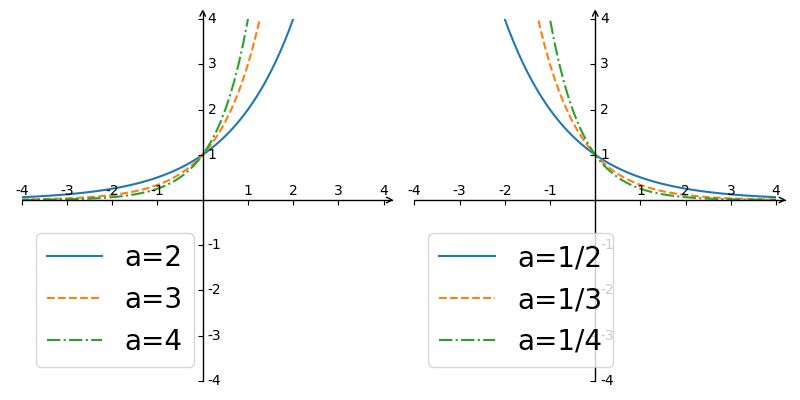
\includegraphics[height=5cm]{4.2-1.png}
\end{figure}

~

\begin{example}[拓广探索9,难度:$\star $]
已知函数
\[
y=a\left( \frac{1}{2} \right) ^{\left| x \right|}+b
\]
图象过原点,且无限接近直线$y=2$但又不与该直线相交。
\begin{enumerate}
    \item 求该函数的解析式,并画出图象;
    \item 判断该函数的奇偶性和单调性。
\end{enumerate}
\end{example}

解:

原函数可化为:
\[
y=\left( \frac{1}{2} \right) ^{\log _{1/2}a}\left( \frac{1}{2} \right) ^{\left| x \right|}+b=\left( \frac{1}{2} \right) ^{\left| x \right|+\log _{1/2}a}+b
\]
对比标准的指数有渐近线$y=0$,这里的渐近线为$y=2$,抬高了2,必然是$b$引起的,所以$b=2$。图象过原点,于是有$0=a+b$,则$a=-2$,最终:
\[
y=-2\left( \frac{1}{2} \right) ^{\left| x \right|}+2
\]
\begin{figure}[h]
\centering
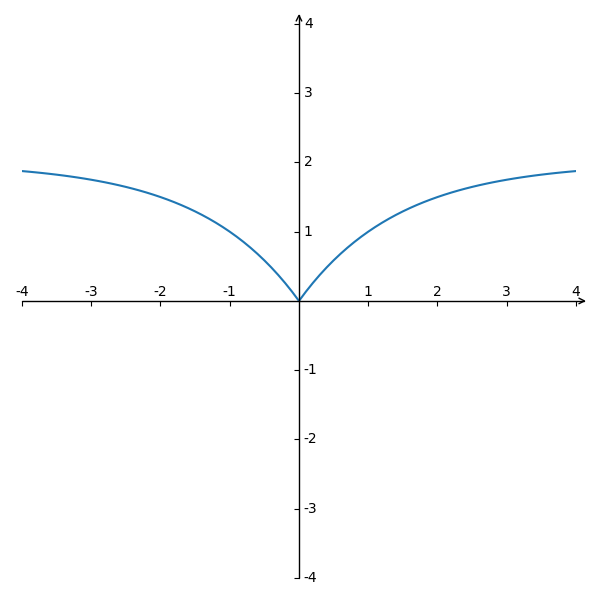
\includegraphics[height=6cm]{4.2-2.png}
\end{figure}

考察$x>0$部分函数图形从标准指数函数演化到题目所示函数的过程,函数化简如下:
\[
y=-2\left( \frac{1}{2} \right) ^x+2=-\left( \frac{1}{2} \right) ^{-1}\left( \frac{1}{2} \right) ^x+2=-\left( \frac{1}{2} \right) ^{x-1}+2
\]
图形分析:
\begin{itemize}
    \item 标准的指数函数$y=\left( 1/2 \right) ^x$;
    \item 右移得到$y=\left( 1/2 \right) ^{x-1}$;
    \item 沿{\it x}轴翻转得到$y=-\left( 1/2 \right) ^{x-1}$;
    \item 上抬2得到$y=-\left( 1/2 \right) ^{x-1}+2$。
\end{itemize}

~

~

~

~

~

~

~

\begin{figure}[ht]
\centering
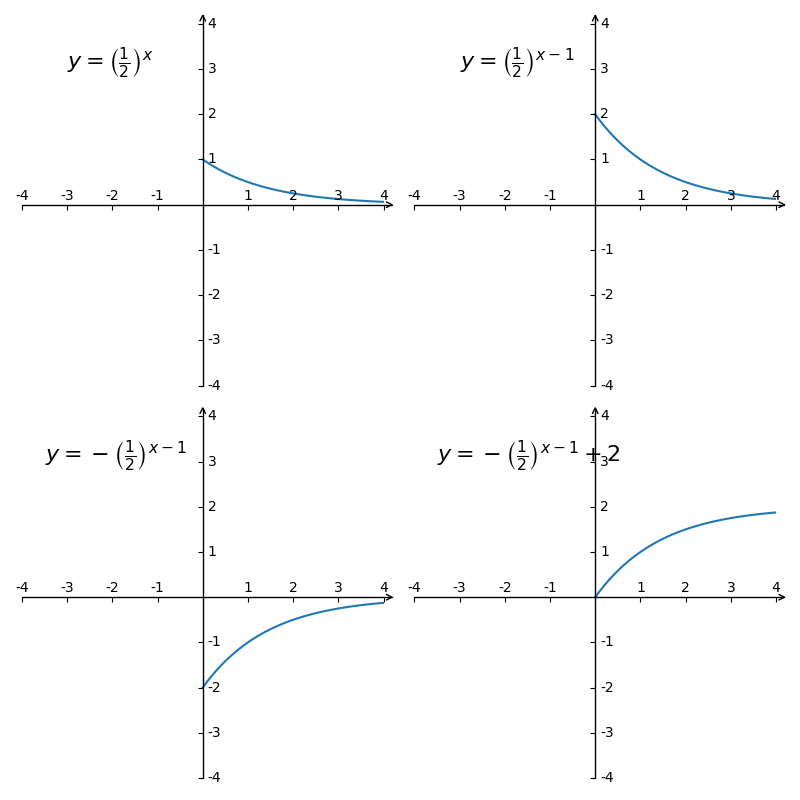
\includegraphics[height=10cm]{4.2-3.png}
\end{figure}

\begin{tcolorbox}
本题其实是对指数函数一次最完整的考察。理解一个函数如何从最基本的形态通过拉伸和平移变得复杂。
\end{tcolorbox}






\newpage
\section{对数}

略。






\newpage
\section{对数函数}

本节要点:
\begin{itemize}
    \item 掌握对数函数的概念及意义;
    \item 熟悉对数函数的图形。
\end{itemize}

~

对数函数
\[
y=\log a^x \qquad a>0\text{且}a\ne 1\quad x\in \mathbb{R} ^+
\]
本身非常简单,没有难度,只需要注意$a$的取值范围。$a=1$时,$y$变成$y=x$没有讨论的意义;$a<0$时,$y$为复数,较为复杂,高中阶段不讨论。

对数函数是指数函数的反函数,所以其意义也很明了,即等比数列达到$x$需要经历的时间。于是,也不难理解:
\begin{itemize}
    \item 对数函数是单调函数,具体看$a$;
    \item 当$a>1$时,单调递增,且$a$越大达到同样的$x$所需的时间越短,曲线越平坦;
    \item 当$a<1$时,单调递减,且$a$越小达到同样的$x$所需的时间越短,曲线越平坦。
\end{itemize}

\begin{figure}[h]
\centering
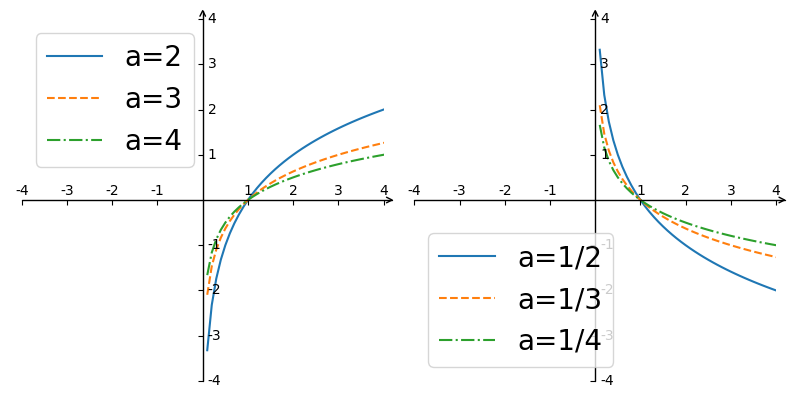
\includegraphics[height=5cm]{4.4-1.png}
\end{figure}






\newpage
\section{函数的应用(二)}

本节没有难度,需要注意几点:
\begin{itemize}
    \item “4.5.1函数的零点与方程的解”中,零点存在定理需要严格定义“连续不断”这个概念,这点在高等数学微积分中展开,高中阶段只是了解该定理;
    \item “4.5.3函数模型的应用”中,马尔萨斯模型的问题在于增长率为常数这个假设并不正确。
\end{itemize}

~

函数模型的应用中,我们首先进行数据的采集,根据数据绘制图形,发掘数据的关系,然后选择合适的模型,可以是幂函数、指数函数、对数函数或者它们的组合,最后根据数据决定未知数,这需要线性代数中的最小二乘法及其衍生方法。当然,还需要对模型进行评判,这需要数理统计中的检验假设的相关知识。高中阶段我们考虑地较为简单,使用单个的标准函数作为模型即可。

\begin{tcolorbox}
还是那个套路,只不过我们原来只有一个框“幂函数”,现在我们多了一个“指数函数”这个框。XML!
\end{tcolorbox}






\newpage
\section{本章小结}

本章介绍了指数函数和对数函数。
关键点:
\begin{itemize}
    \item 指数函数和对数函数可通过等比数列加深理解;
    \item 两者是互为反函数;
    \item 熟悉使用指数函数和对数函数作为模型求解实际问题。
\end{itemize}

~

\begin{example}[复习巩固4,难度:$\star $]
已知函数
\[
f\left( x \right) =\begin{cases}
	x^2+2x-3 &x\leqslant 0\\
	-2+\ln x &x>0\\
\end{cases}
\]
求使方程$f\left( x \right) =k$的实数解个数分别为1、2、3时$k$的相应取值范围。
\end{example}

解:

首先观察
\[
-2+\ln x-k=0 \qquad x>0
\]
即函数$g\left( x \right) =\ln x-\left( k+2 \right) $,相比$\ln x$往下移了$k+2$,无论如何都跟{\it x}轴有且仅有一个交点。所以本题实际为考察
\[
g\left( x \right) =x^2+2x-3-k \qquad x\leqslant 0
\]
与{\it x}轴的交点。
方程化为:
\[
g\left( x \right) =\left( x+1 \right) ^2+\left( -4-k \right)
\]
即将$\left( x+1 \right) ^2$上下平移得到,易得:
\begin{itemize}
    \item $-4-k>0$时,无交点;
    \item $-4-k=0$或$-4-k<-1$时,1个交点;
    \item 其余,2个交点。
\end{itemize}

\begin{tcolorbox}
本题没啥难度,考察幂函数和对数函数的形态而已。
\end{tcolorbox}

~

\begin{example}[拓广探索12,难度:$\star $]
对于函数
\[
f\left( x \right) =a-\frac{2}{2^x+1} \qquad a\in \mathbb{R}
\]
\begin{enumerate}
    \item 探索函数$f\left( x \right) $的单调性;
    \item 是否存在实数$a$使函数$f\left( x \right) $为奇函数?
    \item (附加)证明函数是中心对称。
\end{enumerate}
\end{example}

解:

(1)从定义出发,令$x_1<x_2$,则有:
\begin{align*}
f\left( x_1 \right) -f\left( x_2 \right) &=\frac{2}{2^{x_2}+1}-\frac{2}{2^{x_1}+1}=2\cdot \frac{\left( 2^{x_1}+1 \right) -\left( 2^{x_2}+1 \right)}{\left( 2^{x_2}+1 \right) \left( 2^{x_1}+1 \right)} \\
&=2\cdot \frac{2^{x_1}-2^{x_2}}{\left( 2^{x_2}+1 \right) \left( 2^{x_1}+1 \right)}<0
\end{align*}

(2)若要使$f\left( x \right) $为奇函数,则必须$f\left( -x \right) =-f\left( x \right) $,于是:
\begin{align*}
&\because f\left( -x \right) =a-\frac{2}{2^{-x}+1}=a-\frac{2}{\frac{1}{2^x}+1}=\frac{a\left( 2^x+1 \right) -2\cdot 2^x}{2^x+1} \\
&\because -f\left( x \right) =\frac{-a\left( 2^x+1 \right) +2}{2^x+1} \\
&\therefore \left( a-2 \right) \cdot 2^x+a=-a\cdot 2^x-a+2 \\
&\therefore \left( a-1 \right) \cdot 2^x=-\left( a-1 \right)
\end{align*}
可见,$a=1$即可,带入验证:
\begin{align*}
&f\left( x \right) =1-\frac{2}{2^x+1}=\frac{2^x-1}{2^x+1} \\
&f\left( -x \right) =\frac{2^{-x}-1}{2^{-x}+1}=\frac{\frac{1}{2^x}-\frac{2^x}{2^x}}{\frac{1}{2^x}+\frac{2^x}{2^x}}=\frac{1-2^x}{1+2^x}
\end{align*}

\begin{figure}[h]
\centering
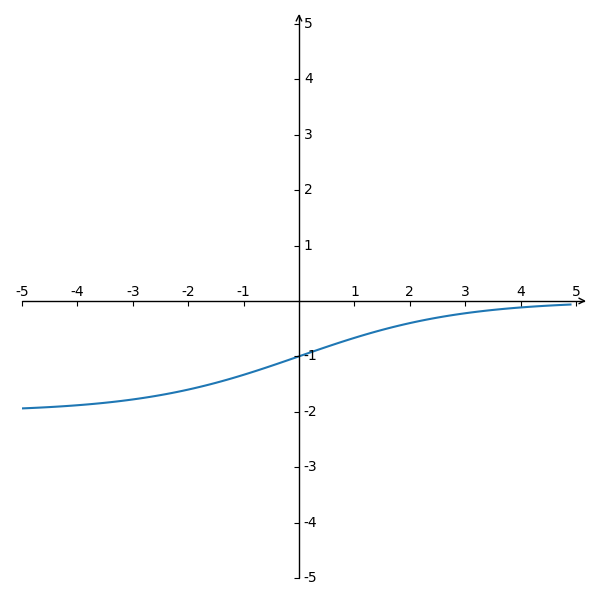
\includegraphics[height=6cm]{4.6-1.png}
\end{figure}

(3)中心对称即若有$x_1+x_2=2x_0$则有$y_1+y_2=2y_0$,带入计算:
\begin{align*}
y_1+y_2&=a-\frac{2}{2^{x_1}+1}+a-\frac{2}{2^{x_2}+1} \\
&=2a-2\cdot \frac{2^{x_1}+2^{x_2}+2}{2^{x_1+x_2}+2^{x_1}+2^{x_2}+1}
\end{align*}
可见,当$x_1+x_2=0$时,有$y_1+y_2=2a-2$,也即中心点$\left( 0,2a-2 \right) $。

回头再看(2),只需要上抬就可以满足奇函数要求。

\begin{tcolorbox}
本题从定义出发即可。
本题的附加(3)类似2024年高考第18题。
\end{tcolorbox}










\chapter{三角函数}

本章介绍三角函数。三角函数是一个重点,但不是难点。说重点,是因为三角函数公式多,计算量特别大,容易出大题。不是难点,是因为三角函数作为函数的一个类型,并没有脱离第一章的范式,而且三角函数和直角坐标是等价的,我们可以借助直角坐标求解问题。

本章要点:
\begin{itemize}
    \item 三角函数。
\end{itemize}

\newpage
\section{任意角和弧度制}

略。

都是定义,没啥难点。估计弧度制有些不适应。这么想,若要用函数的方法考察角度,那么角度不是自变量就是应变量,那么你还会希望角度只能是有理数吗?角度制只能是有理数,而弧度制能使角度这个变量成为实数。






\newpage
\section{三角函数的概念}

本节要点:
\begin{itemize}
    \item 掌握3个三角函数的概念。
\end{itemize}

~

首先,所谓的三角函数,关键其实只有两个,$\sin ,\cos $,其余都是根据这两个推广得到的。
\begin{align*}
&\sin \alpha =\frac{y}{R} \\
&\cos \alpha =\frac{x}{R}
\end{align*}

其次,三角函数联系了直角坐标系和极坐标系,这两个坐标系是等价的,既然是等价的。而且从定义不难发现,这2个三角函数完全可以认为是$x,y,R$的代替,所以有些问题可以转成$x,y,R$分析。

~

\begin{example}[综合运用14(2),难度:$\star $]
求证:$\tan ^2\alpha -\sin ^2\alpha =\tan ^2\alpha \sin ^2\alpha $。
\end{example}

解:

左边:
\[
\tan ^2\alpha -\sin ^2\alpha =\left( \frac{y}{x} \right) ^2-\left( \frac{y}{R} \right) ^2=\frac{y^2}{x^2}-\frac{y^2}{x^2+y^2}
\]

右边:
\[
\tan ^2\alpha \sin ^2\alpha =\left( \frac{y}{x} \right) ^2\left( \frac{y}{R} \right) ^2=\frac{y^2}{x^2}\cdot \frac{y^2}{R^2}=\frac{y^2}{x^2}\cdot \frac{y^2}{x^2+y^2}
\]

略。

\begin{tcolorbox}
可见,转成$x,y,R$非常简单。
\end{tcolorbox}






\newpage
\section{诱导公式}

本节要点:
\begin{itemize}
    \item 熟练掌握诱导公式。
\end{itemize}

~

教材中从公式二到公式六,其实总结起来就4类。

{\bf 周期性}
\begin{align*}
&\sin \left( \alpha +2\pi \right) =\sin \alpha \\
&\cos \left( \alpha +2\pi \right) =\cos \alpha \\
&\tan \left( \alpha +2\pi \right) =\tan \alpha
\end{align*}

{\bf 半周期性}
\begin{align*}
&\sin \left( \alpha +\pi \right) =-\sin \alpha \\
&\cos \left( \alpha +\pi \right) =-\cos \alpha \\
&\tan \left( \alpha +\pi \right) =\tan \alpha
\end{align*}

{\bf 奇偶性}
\begin{align*}
&\sin \left( -\alpha \right) =-\sin \alpha \\
&\cos \left( -\alpha \right) =\cos \alpha \\
&\tan \left( -\alpha \right) =-\tan \alpha
\end{align*}

{\bf 互换}
\begin{align*}
&\sin \left( \alpha +\frac{\pi}{2} \right) =\cos \alpha \\
&\cos \left( \alpha +\frac{\pi}{2} \right) =-\sin \alpha
\end{align*}






\newpage
\section{三角函数的图象与性质}

略。






\newpage
\section{三角恒等变换}

本节要点:
\begin{itemize}
    \item 熟练掌握变换公式。
\end{itemize}

~

{\bf 和差角}
\begin{align*}
&\sin \left( \alpha \pm \beta \right) =\sin \alpha \cos \beta \pm \cos \alpha \sin \beta \\
&\cos \left( \alpha \pm \beta \right) =\cos \alpha \cos \beta \mp \sin \alpha \sin \beta \\
&\tan \left( \alpha \pm \beta \right) =\frac{\tan \alpha \pm \tan \beta}{1\mp \tan \alpha \tan \beta}
\end{align*}

{\bf 二倍角}
\begin{align*}
&\sin 2\alpha =2\sin \alpha \cos \alpha \\
&\cos 2\alpha =\cos ^2\alpha -\sin ^2\alpha =2\cos ^2\alpha -1=1-2\sin ^2\alpha \\
&\tan 2\alpha =\frac{2\tan \alpha}{1-\tan ^2\alpha}
\end{align*}

{\bf 和差化积}
\begin{align*}
&\sin \alpha +\sin \beta =2\sin \left( \frac{\alpha +\beta}{2} \right) \cos \left( \frac{\alpha -\beta}{2} \right) \\
&\sin \alpha -\sin \beta =2\cos \left( \frac{\alpha +\beta}{2} \right) \sin \left( \frac{\alpha -\beta}{2} \right) \\
&\cos \alpha +\cos \beta =2\cos \left( \frac{\alpha +\beta}{2} \right) \cos \left( \frac{\alpha -\beta}{2} \right) \\
&\cos \alpha -\cos \beta =-2\sin \left( \frac{\alpha +\beta}{2} \right) \sin \left( \frac{\alpha -\beta}{2} \right)
\end{align*}

{\bf 积化和差}
\begin{align*}
&\sin \alpha \cos \beta =\frac{1}{2}\left[ \sin \left( \alpha +\beta \right) +\sin \left( \alpha -\beta \right) \right] \\
&\cos \alpha \sin \beta =\frac{1}{2}\left[ \sin \left( \alpha +\beta \right) -\sin \left( \alpha -\beta \right) \right] \\
&\cos \alpha \cos \beta =\frac{1}{2}\left[ \cos \left( \alpha +\beta \right) +\cos \left( \alpha -\beta \right) \right] \\
&\sin \alpha \sin \beta =-\frac{1}{2}\left[ \cos \left( \alpha +\beta \right) -\cos \left( \alpha -\beta \right) \right]
\end{align*}






\newpage
\section{函数\texorpdfstring{$y=A\sin \left( \omega x+\varphi \right) $}\ }

本节要点:
\begin{itemize}
    \item 结合图形理解函数的各个部分。
\end{itemize}

~

本章前5节都把三角函数作为公式看待,本节开始将三角函数作为函数考察。
\[
y=A\sin \left( \omega x+\varphi \right)
\]

我们从最简单的形式开始
\[
y=\sin x
\]
这里,引申出一个概念,我们将$x$称为{\bf 相位}(phase)。所谓的相位,就是相的位置,所谓的相,就是$y$,$y$会随着$x$的不同位置呈现出不同的样子。

我们将图象进行沿{\it x}轴平移,得到
\[
y=\sin \left( x+\varphi \right)
\]
这里,又引申出一个概念,我们将$\varphi $称为{\bf 初相},即初始相位。

第三步,我们将图象进行拉伸,得到
\[
y=\sin \left( \omega x+\varphi \right)
\]
这里,再引申出一个概念,由于三角函数的周期性,有:
\[
\omega \left( x+\frac{2\pi}{\omega} \right) +\varphi =\omega x+2\pi +\varphi
\]
也即函数的周期为$T=2\pi /\omega $,我们将其倒数称为角频$f=\frac{\omega}{2\pi}$。

最后,将图象沿{\it y}轴拉伸,得到
\[
y=A\sin \left( \omega x+\varphi \right)
\]
我们称$A$为振幅。






\newpage
\section{三角函数的应用}

略。

~

这里稍微扩展一点。三角函数是描述周期性运动的必然选择,这是由微分方程决定的。

从能量守恒的角度,如弹簧构成的谐振子,有如下形式
\[
f\left( x^2 \right) +g\left( y^2 \right) =C
\]
$x,y$必然可以通过参数方程转化为三角函数的形式。

从线性代数的角度看,三角函数构成了一组正交基,能描述常见的函数,这就是傅里叶变换。






\newpage
\section{本章小结}

本章介绍了三角函数:
\begin{itemize}
    \item 为了使三角公式顺利进展到三角函数,5.1先引入了弧度制;
    \item 5.2顺势定义了3个基本的三角公式;
    \item 5.3~5.5说的就是一件事,即推导$f\left( x_1+x_2 \right) $;
    \item 5.6~5.7将三角公式推广到三角函数。
\end{itemize}

~

\begin{example}[综合运用23,难度:$\star $]
如图,正方形$ABCD$的边长为1,$P,Q$分别为边$AB,DA$上的点,当$\bigtriangleup APQ$的周长为2时,求$\angle PCQ$的大小。
\end{example}

解一:

\begin{figure}[h]
\centering
\begin{tikzpicture}[line join=round, scale=3]
\mydrawsquare[1]{A}{B}{C}{D}
\coordinate[label=below:{$P$}] (P) at ($(A)!0.4!(B)$);
\coordinate[label=left: {$Q$}] (Q) at ($(A)!0.6!(D)$);
\draw[thick,blue] (Q)--(P)--(C)--(Q);
\coordinate[label=left: {$x$}]   (x)  at ($(A)!0.5!(Q)$);
\coordinate[label=left: {$1-x$}] (x') at ($(Q)!0.5!(D)$);
\coordinate[label=below:{$y$}]   (y)  at ($(A)!0.5!(P)$);
\coordinate[label=below:{$1-y$}] (y') at ($(P)!0.5!(B)$);
\coordinate[label=above:{$1$}]   (t1) at ($(D)!0.5!(C)$);
\coordinate[label=right:{$1$}]   (t2) at ($(C)!0.5!(B)$);
\coordinate[label=below:{$\sqrt{1+\left( 1-x \right) ^2}$}] (t3) at ($(C)!0.5!(Q)$);
\coordinate[label=below:{$\sqrt{1+\left( 1-y \right) ^2}$}] (t4) at ($(C)!0.5!(P)$);
\coordinate[label=below:{$\sqrt{x^2+y^2}$}]                 (t5) at ($(Q)!0.5!(P)$);
\pic["$\theta $",draw,angle radius=0.5cm,angle eccentricity=1.5] {angle=Q--C--P};
\end{tikzpicture}
\end{figure}

如上图设置。根据$\bigtriangleup APQ$的周长为2可得:
\begin{align*}
&\because x+y+\sqrt{x^2+y^2}=2 \\
&\therefore x^2+y^2=\left[ 2-\left( x+y \right) \right] ^2=4-4x-4y+x^2+2xy+y^2 \\
&\therefore 2x+2y=2+xy \\
&\therefore 4x^2+8xy+4y^2=4+4xy+x^2y^2 \\
&\therefore 4x^2+4y^2=4-4xy+x^2y^2=\left( 2-xy \right) ^2
\end{align*}
也即:
\[
x+y=\frac{2+xy}{2} \qquad x^2+y^2=\frac{\left( 2-xy \right) ^2}{4}
\]

使用余弦定理可得:
\[
\cos \theta =\frac{CQ^2+CP^2-PQ^2}{2\cdot CQ\cdot CP}
\]
分子的化简较为简单:
\begin{align*}
&=\left[ 1+\left( 1-x \right) ^2 \right] +\left[ 1+\left( 1-y \right) ^2 \right] -\left( x^2+y^2 \right) \\
&=4-2x-2y \\
&=4-2\cdot \frac{2+xy}{2} \\
&=2-xy
\end{align*}
分母的化简较为复杂,下面略去了很多步骤:
\begin{align*}
&=2\sqrt{1+\left( 1-x \right) ^2}\sqrt{1+\left( 1-y \right) ^2} \\
&=2\sqrt{\left[ 1+\left( 1-x \right) ^2 \right] \left[ 1+\left( 1-y \right) ^2 \right]} \\
&=2\sqrt{4-4x-4y+2x^2+4xy-2x^2y+2y^2-2xy^2+x^2y^2} \\
&=2\sqrt{4-4\left( x+y \right) +2\left( x^2+y^2 \right) +4xy+x^2y^2-2xy\left( x+y \right)} \\
&=2\sqrt{\frac{\left( 2-xy \right) ^2}{2}}
\end{align*}
最终得:
\[
\cos \theta =\frac{2-xy}{2\sqrt{\frac{\left( 2-xy \right) ^2}{2}}}=\frac{1}{\sqrt{2}}
\]

解二:

\begin{figure}[h]
\centering
\begin{tikzpicture}[line join=round, scale=3]
\mydrawsquare[1]{A}{B}{C}{D}
\coordinate[label=below:{$P$}] (P) at ($(A)!0.4!(B)$);
\coordinate[label=left: {$Q$}] (Q) at ($(A)!0.6!(D)$);
\draw[thick,blue] (Q)--(P)--(C)--(Q);
\coordinate[label=left: {$x$}]   (x)  at ($(A)!0.5!(Q)$);
\coordinate[label=left: {$1-x$}] (x') at ($(Q)!0.5!(D)$);
\coordinate[label=below:{$y$}]   (y)  at ($(A)!0.5!(P)$);
\coordinate[label=below:{$1-y$}] (y') at ($(P)!0.5!(B)$);
\pic["$\alpha $",draw,angle radius=0.7cm,angle eccentricity=1.5] {angle=D--C--Q};
\pic["$\theta $",draw,angle radius=0.5cm,angle eccentricity=1.5] {angle=Q--C--P};
\pic["$\beta $",draw,angle radius=0.6cm,angle eccentricity=1.5] {angle=P--C--B};
\end{tikzpicture}
\end{figure}

如上图设置,考察$\alpha +\beta$:
\begin{align*}
\tan \left( \alpha +\beta \right) &=\frac{\tan \alpha +\tan \beta}{1-\tan \alpha \tan \beta}=\frac{\left( 1-x \right) +\left( 1-y \right)}{1-\left( 1-x \right) \left( 1-y \right)} \\
&=\frac{2-x-y}{x+y-xy}
\end{align*}
由周长条件可得$2x+2y=2+xy$,带入:
\[
\tan \left( \alpha +\beta \right) =\frac{2-x-y}{x+y-\left( 2x+2y-2 \right)}=1
\]

\begin{tcolorbox}
解一使用余弦定理暴力计算,计算量大,思路明确。解二通过把角拆分,配合正切公式,计算量小非常多。
\end{tcolorbox}










\chapter{平面向量及其应用}

本章介绍平面上的向量。有两个难点,第一,平面向量是第一次碰到,难以快速熟悉并掌握,需要花大力气,其次,向量是连接代数和几何的桥梁,容易出大题,计算量可大可小。所以平面向量的学习需要反复研读定义,深刻理解定义提出的背景,还须结合几何,多画图,借助图形展开思考。

本章要点:
\begin{itemize}
    \item 平面向量及其几何意义。
    \item 余弦定理和正弦定理。
\end{itemize}

\newpage
\section{平面向量的概念}

都是定义,没啥难点。向量就是带方向的量。

可以这么理解,如果描述一维空间的坐标,则使用标量即可,没有方向,或者只有两个方向,前后,用实数的正负即可。如果描述二维空间的坐标,则必须使用两个标量,组合在一起就是向量。

教材中说道向量的三元素:起点、方向、长度。其实只有方向和长度,我们不太关心起点,起点是可以移动的。从后续的平行和相等的定义也可以看出,起点并没有要求。

这里容易忽略一个关键点,即模和方向是向量的固有属性。所谓的固定属性就是它们不随参考系的变化而变化,这点在学习到第3节的时候需要特别注意!XML。






\newpage
\section{平面向量的运算}

本节要点:
\begin{itemize}
    \item 掌握向量的运算的概念;
    \item 掌握向量的运算法则;
    \item 理解向量运算的几何意义。
\end{itemize}

\begin{tcolorbox}
本节将向量作为一个整体,或者说将向量作为一个一类数,定义了运算法则。下一节将向量和实数关联讨论运算法则,注意这两节的区别。
\end{tcolorbox}

本节对向量的运算做了定义,特别是内积,“6.2.4向量的数量积”定义了内积,这个概念是实数没有的,需要熟悉,把该小节的所有例题全部吃透!反复吃透!

加法的交换律和结合律:
\begin{align*}
&\boldsymbol{a}+\boldsymbol{b}=\boldsymbol{b}+\boldsymbol{a} \\
&\left( \boldsymbol{a}+\boldsymbol{b} \right) +\boldsymbol{c}=\boldsymbol{a}+\left( \boldsymbol{b}+\boldsymbol{c} \right)
\end{align*}

数乘的结合律和分配律:
\begin{align*}
&\lambda \left( \mu \boldsymbol{a} \right) =\left( \lambda \mu \right) \boldsymbol{a} \\
&\left( \lambda +\mu \right) \boldsymbol{a}=\lambda \boldsymbol{a}+\mu \boldsymbol{a} \\
&\lambda \left( \boldsymbol{a}+\boldsymbol{b} \right) =\lambda \boldsymbol{a}+\lambda \boldsymbol{b}
\end{align*}

内积的交换律和分配律,特别注意,内积没有结合律:
\begin{align*}
&\boldsymbol{a}\cdot \boldsymbol{b}=\boldsymbol{b}\cdot \boldsymbol{a} \\
&\boldsymbol{a}\cdot \left( \boldsymbol{b}+\boldsymbol{c} \right) =\boldsymbol{a}\cdot \boldsymbol{b}+\boldsymbol{a}\cdot \boldsymbol{c}
\end{align*}

两个重要的不等式:
\begin{itemize}
    \item $\left| \boldsymbol{a}+\boldsymbol{b} \right|\leqslant \left| \boldsymbol{a} \right|+\left| \boldsymbol{b} \right|$,当且仅当$\boldsymbol{a},\boldsymbol{c}$同向时等号成立;
    \item $\left| \boldsymbol{a}\cdot \boldsymbol{b} \right|\leqslant \left| \boldsymbol{a} \right|\cdot \left| \boldsymbol{b} \right|$,当且仅当$\boldsymbol{a},\boldsymbol{c}$平行时等号成立。
\end{itemize}

两个与几何相关的判断,也即数乘和内积的几何意义:
\begin{itemize}
    \item $\boldsymbol{a}=\lambda \boldsymbol{b},\lambda \ne 0\Leftrightarrow \boldsymbol{a},\boldsymbol{b}\text{平行}$;
    \item $\boldsymbol{a}\cdot \boldsymbol{b}=0\Leftrightarrow \boldsymbol{a},\boldsymbol{b}\text{垂直}$。
\end{itemize}

\begin{tcolorbox}
向量是联系代数和几何的有力工具,所以必须深刻理解向量及其运算的几何意义。向量描述了几何的点,向量的集合便是点的集合,可以构成直线、圆、弧、曲线等等。向量的运算描述了这些点和线的关系。
\end{tcolorbox}

\begin{tcolorbox}
教材从力的做功定义向量内积,略有唐突,但考虑到高中阶段背景知识也只能如此。其实向量的相乘还有一个外积,两个积合起来还有更深刻的物理意义,XML。
\end{tcolorbox}

~

\begin{example}[复习巩固7]
已知$\boldsymbol{a},\boldsymbol{b}$为两个非零向量,
\begin{enumerate}
    \item 求作向量$\boldsymbol{a}+\boldsymbol{b},\boldsymbol{a}-\boldsymbol{b}$;
    \item 当向量$\boldsymbol{a},\boldsymbol{b}$成什么位置关系时,满足$\left| \boldsymbol{a}+\boldsymbol{b} \right|=\left| \boldsymbol{a}-\boldsymbol{b} \right|$?(不要求证明)。
\end{enumerate}
\end{example}

解:

只讨论(2),直觉发现要求$\boldsymbol{a}\bot \boldsymbol{b}$。由于涉及向量的坐标表示,所以这里不要求证明,但我们在学习完6.3后回头再证明该题。
令$\boldsymbol{a}=\left( x_{\boldsymbol{a}},y_{\boldsymbol{a}} \right) ,\boldsymbol{b}=\left( x_{\boldsymbol{b}},y_{\boldsymbol{b}} \right) $,可得:
\begin{align*}
&\because \left| \boldsymbol{a}+\boldsymbol{b} \right|=\left| \boldsymbol{a}-\boldsymbol{b} \right| \\
&\therefore \left( x_{\boldsymbol{a}}+x_{\boldsymbol{b}} \right) ^2+\left( y_{\boldsymbol{a}}+y_{\boldsymbol{b}} \right) ^2=\left( x_{\boldsymbol{a}}-x_{\boldsymbol{b}} \right) ^2+\left( y_{\boldsymbol{a}}-y_{\boldsymbol{b}} \right) ^2 \\
&\therefore 2x_{\boldsymbol{a}}x_{\boldsymbol{b}}+2y_{\boldsymbol{a}}y_{\boldsymbol{b}}=-2x_{\boldsymbol{a}}x_{\boldsymbol{b}}-2y_{\boldsymbol{a}}y_{\boldsymbol{b}} \\
&\therefore x_{\boldsymbol{a}}x_{\boldsymbol{b}}+y_{\boldsymbol{a}}y_{\boldsymbol{b}}=0 \\
&\therefore \boldsymbol{a}\cdot \boldsymbol{b}=0
\end{align*}

~

\begin{example}[复习巩固12,难度:$\star $]
求证:
\[
\left( \lambda \boldsymbol{a} \right) \cdot \boldsymbol{b}=\lambda \left( \boldsymbol{a}\cdot \boldsymbol{b} \right) =\boldsymbol{a}\cdot \left( \lambda \boldsymbol{b} \right)
\]
\end{example}

解:

只证明第一个等号:
\begin{align*}
&\left( \lambda \boldsymbol{a} \right) \cdot \boldsymbol{b}=\left| \lambda \boldsymbol{a} \right|\cdot \left| \boldsymbol{b} \right|\cdot \cos \alpha =\left| \lambda \right|\cdot \left| \boldsymbol{a} \right|\cdot \left| \boldsymbol{b} \right|\cdot \cos \alpha \\
&\lambda \left( \boldsymbol{a}\cdot \boldsymbol{b} \right) =\lambda \left( \left| \boldsymbol{a} \right|\cdot \left| \boldsymbol{b} \right|\cdot \cos \alpha \right)
\end{align*}
再从$\lambda <0,>0,=0$三个方面讨论即可,略。

\begin{tcolorbox}
该关系式是内积的性质,证明性质,都从定义入手。
\end{tcolorbox}

~

\begin{example}[拓广探索23,难度:$\star $]
已知$O$为平行四边形$ABCD$所在平面内一点,且向量$\overrightarrow{OA},\overrightarrow{OC},\overrightarrow{OB},\overrightarrow{OD}$满足等式$\overrightarrow{OA}+\overrightarrow{OC}=\overrightarrow{OB}+\overrightarrow{OD}$。
\begin{enumerate}
    \item 做出满足条件的四边形$ABCD$。
    \item 四边形$ABCD$有什么特点?请证明你的猜想。
\end{enumerate}
\end{example}

\begin{figure}[h]
\centering
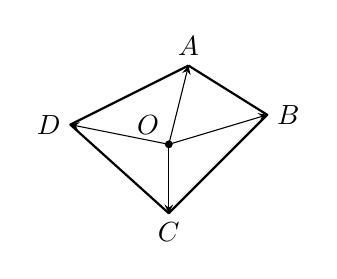
\begin{tikzpicture}[line join=round, scale=1.25]
\pgfmathparse{0.6/1.5}
\coordinate[label=above left:{$O$}] (O) at (0,0);
\coordinate[label=left:{$D$}] (D) at (-1,0.2);
\coordinate[label=right:{$B$}] (B) at (1,0.3);
\coordinate[label=below:{$C$}] (C) at (0,-0.7);
\coordinate[label=above:{$A$}] (A) at (0.2,0.8);
\fill (O) circle (\pgfmathresult mm);
\draw[thick] (A)--(B)--(C)--(D)--(A);
\draw[-stealth] (O)--(A);
\draw[-stealth] (O)--(B);
\draw[-stealth] (O)--(C);
\draw[-stealth] (O)--(D);
\end{tikzpicture}
\end{figure}

解:

$\overrightarrow{OA}+\overrightarrow{OC}$表示两向量和,但几何上起点相同,所以很难由此判断出四边形的特点,最好是首尾相连,且去掉$O$。
将等式变换化简:
\begin{align*}
&\overrightarrow{OA}+\overrightarrow{OC}=\overrightarrow{OB}+\overrightarrow{OD} \\
&\overrightarrow{OA}-\overrightarrow{OB}=\overrightarrow{OD}-\overrightarrow{OC} \\
&\overrightarrow{BO}+\overrightarrow{OA}=\overrightarrow{CO}+\overrightarrow{OD} \\
&\overrightarrow{BA}=\overrightarrow{CD}
\end{align*}
对边相等且平行,易得为平行四边形。

\begin{tcolorbox}
此题考察向量运算的几何意义,粗看较为抽象,但依然有思路可循。
\end{tcolorbox}

~

\begin{example}[拓广探索24,难度:$\star $]
如图,在$\odot C$中,是不是只需知道$\odot C$的半径或弦$AB$的长度,就可以求出$\overrightarrow{AB}\cdot \overrightarrow{AC}$的值?
\end{example}

\begin{figure}[h]
\centering
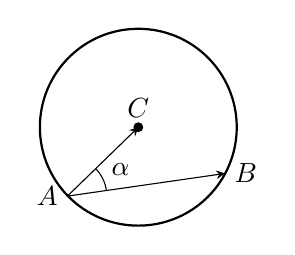
\begin{tikzpicture}[line join=round, scale=1.25]
\pgfmathparse{0.6/1.2}
\draw[thick] (0,0) circle(1);
\coordinate[label=above:{$C$}] (C) at (0,0);
\coordinate[label=left: {$A$}] (A) at (-0.72,-0.7);
\coordinate[label=right:{$B$}] (B) at (0.88,-0.47);
\fill (C) circle (\pgfmathresult mm);
\draw[-stealth] (A)--(C);
\draw[-stealth] (A)--(B);
\pic["$\alpha $",draw,angle radius=0.5cm,angle eccentricity=1.5] {angle=B--A--C};
\end{tikzpicture}
\end{figure}

解:

\begin{align*}
&\because \overrightarrow{AB}\cdot \overrightarrow{AC}=\left| \overrightarrow{AB} \right|\cdot \left| \overrightarrow{AC} \right|\cdot \cos \alpha \\
&\because \cos \alpha =\frac{\left| \overrightarrow{AC} \right|^2+\left| \overrightarrow{AB} \right|^2-\left| \overrightarrow{CB} \right|^2}{2\cdot \left| \overrightarrow{AC} \right|\cdot \left| \overrightarrow{AB} \right|} \\
&\because \left| \overrightarrow{AC} \right|=\left| \overrightarrow{CB} \right| \\
&\therefore \overrightarrow{AB}\cdot \overrightarrow{AC}=\frac{\left| \overrightarrow{AB} \right|^2}{2}
\end{align*}

略。

\begin{tcolorbox}
从向量内积的定义出发,结合余弦定理即可,非常简单。
\end{tcolorbox}






\newpage
\section{平面向量基本定理及坐标表示}

本节要点:
\begin{itemize}
    \item 理解向量的坐标表示;
    \item 熟练掌握向量运算的坐标表示。
\end{itemize}

\begin{tcolorbox}
本节将向量分解为实数的有序组合,并定义运算法则。
\end{tcolorbox}

本节的概念较为复杂,新概念多,新写法多,再次作梳理总结。

首先,高中阶段讨论的向量是二维向量,几何上表示二维平面的有向线段,在{\it xy}坐标系中,原点和任意点也能构成的有向线段。加之“平面向量定理”,我们可以证明二维平面和{\it xy}坐标系是同构的。所以,以下向量的表示方法是等价的:
\begin{itemize}
    \item $\overrightarrow{AB}$:表示二维空间的有向线段;
    \item $x\boldsymbol{i}+y\boldsymbol{j}$:表示{\it xy}坐标系中的有向线段;
    \item $\left( x,y \right) $:表示{\it xy}坐标系中的点。
\end{itemize}
综合表示如下,注意,这里的=表示含义等价,而非代数中的等量:
\[
\boldsymbol{a}=\overrightarrow{AB}=x\boldsymbol{i}+y\boldsymbol{j}=\left( x,y \right)
\]
仔细研读本节所有例题,理解上述关系式。

于是我们不难得到:
\begin{align*}
&\boldsymbol{a}+\boldsymbol{b}=\overrightarrow{AB}=\left( x_{\boldsymbol{a}}+x_{\boldsymbol{b}} \right) \boldsymbol{i}+\left( y_{\boldsymbol{a}}+y_{\boldsymbol{b}} \right) \boldsymbol{j}=\left( x_{\boldsymbol{a}}+x_{\boldsymbol{b}},y_{\boldsymbol{a}}+y_{\boldsymbol{b}} \right) \\
&\lambda \boldsymbol{a}=\lambda x_{\boldsymbol{a}}\boldsymbol{i}+\lambda y_{\boldsymbol{a}}\boldsymbol{j}=\left( \lambda x_{\boldsymbol{a}},\lambda y_{\boldsymbol{a}} \right) \\
&\boldsymbol{a}\cdot \boldsymbol{b}=\left( x_{\boldsymbol{a}}\boldsymbol{i}+y_{\boldsymbol{a}}\boldsymbol{j} \right) \cdot \left( x_{\boldsymbol{b}}\boldsymbol{i}+y_{\boldsymbol{b}}\boldsymbol{j} \right) =x_{\boldsymbol{a}}\cdot x_{\boldsymbol{b}}+y_{\boldsymbol{a}}\cdot y_{\boldsymbol{b}}=\left| \boldsymbol{a} \right|\left| \boldsymbol{b} \right|\cos \alpha
\end{align*}

\begin{tcolorbox}
本节将向量用一个有序实数对表示,并根据之前的定义完善了向量的运算,使得向量彻底关联了代数和几何。
\end{tcolorbox}

\begin{figure}[h]
\centering
\begin{minipage}{.49\textwidth}
\centering
\begin{tikzpicture}[line join=round, scale=1]
\coordinate (x1) at (-1,0);
\coordinate (y1) at (-0.5,-1);
\coordinate[label=right:{$x$}] (x2) at (1,0);
\coordinate[label=above:{$y$}] (y2) at (0.5,1);
\draw[->,red] (x1)--(x2);
\draw[->,red] (y1)--(y2);
\end{tikzpicture}
\end{minipage}
\begin{minipage}{.49\textwidth}
\centering
\begin{tikzpicture}[line join=round, scale=1]
\mydrawxy{-1}{1}{-1}{1}
\end{tikzpicture}
\end{minipage}
\end{figure}

还有一个问题需要注意,教材中未提及。坐标系可以多种多样,只要两个坐标轴不重合即可构建二维坐标系,如上左图,若约束{\it xy}垂直,就构成正交坐标系,也即我们熟知的笛卡尔坐标系,如上右图。

之前在6.1中我提及,模是向量的固有属性,所以要计算$\boldsymbol{a}=\left( x,y \right) $的模,这里的$x,y$必须是正交坐标系下的坐标!高中教材不对模下一个明确的定义,这部分在《线性代数》中定义,所以这里只要知道模的计算需要放在直角坐标系下即可。

\begin{tcolorbox}
高中阶段的向量是简化版的线性代数,XML。
\end{tcolorbox}

~

\begin{example}[复习巩固9,难度:$\star $]
已知$\left| \boldsymbol{a} \right|=3,\boldsymbol{b}=\left( 1,2 \right) $,且$\boldsymbol{a}\parallel \boldsymbol{b}$,求$\boldsymbol{a}$的坐标。
\end{example}

解:

令$\boldsymbol{a}=\left( x,y \right) $,则有:
\begin{align*}
&x^2+y^2=9 \\
&\left( x,y \right) =\lambda \left( 1,2 \right)
\end{align*}
第2个式子表示$\left( x,y \right) =\lambda \left( 1,2 \right) $,不难解得:
\[
\boldsymbol{a}=\pm \left( \frac{3}{\sqrt{5}},\frac{6}{\sqrt{5}} \right)
\]

\begin{tcolorbox}
本题考察向量的性质,并不难。
\end{tcolorbox}

~

\begin{example}[复习巩固10,难度:$\star $]
已知$\boldsymbol{a}=\left( 4,2 \right) $,求与$\boldsymbol{a}$垂直的单位向量的坐标。
\end{example}

解:

与一个向量垂直,约束了其方向,单位向量,约束了其大小,不难发现该题必然得到两个方程:
\begin{align*}
&\boldsymbol{a}\cdot \boldsymbol{b}=0 \\
&\left| \boldsymbol{b} \right|=1
\end{align*}
令$\boldsymbol{b}=\left( x,y \right) $可求解,略。

\begin{tcolorbox}
本题依然考察向量的性质,并不难。
\end{tcolorbox}

~

\begin{example}[综合运用14,难度:$\star $]
求证:以$A\left( 1,0 \right) $,$B\left( 5,-2 \right) $,$C\left( 8,4 \right) $,$D\left( 4,6 \right) $为顶点的四边形是一个矩形。
\end{example}

\begin{figure}[h]
\centering
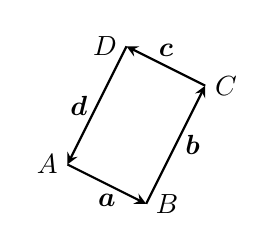
\begin{tikzpicture}[line join=round, scale=0.25]
\mydrawxy{-3}{10}{-3}{8}
\coordinate[label=left: {$A$}]              (A) at (1,0);
\coordinate[label=right:{$B$}]              (B) at (5,-2);
\coordinate[label=right:{$C$}]              (C) at (8,4);
\coordinate[label=left: {$D$}]              (D) at (4,6);
\coordinate[label=below:{$\boldsymbol{a}$}] (a) at ($(A)!0.5!(B)$);
\coordinate[label=right:{$\boldsymbol{b}$}] (b) at ($(B)!0.5!(C)$);
\coordinate[label=above:{$\boldsymbol{c}$}] (c) at ($(C)!0.5!(D)$);
\coordinate[label=left: {$\boldsymbol{d}$}] (d) at ($(D)!0.5!(A)$);
\draw[thick,-stealth] (A)--(B);
\draw[thick,-stealth] (B)--(C);
\draw[thick,-stealth] (C)--(D);
\draw[thick,-stealth] (D)--(A);
\end{tikzpicture}
\end{figure}

解:

从矩形的定义出发,有一个角是直角的平行四边形。
可令向量$\boldsymbol{a},\boldsymbol{b},\boldsymbol{c},\boldsymbol{d}$如上图,不难发现,只需证明:
\begin{align*}
&\boldsymbol{a}=\lambda \boldsymbol{c} \\
&\boldsymbol{a}\cdot \boldsymbol{b}=0
\end{align*}
略。

\begin{tcolorbox}
本题考察向量运算的几何意义,并不难。
\end{tcolorbox}

~

\begin{example}[拓广探索15,难度:$\star $]
如图,$Ox,Oy$是平面内相交成60°角的两条数轴,$\boldsymbol{e}_1,\boldsymbol{e}_2$分别是与{\it x}轴、{\it y}轴正方向通向的单位向量。若向量$\overrightarrow{OP}=x\boldsymbol{e}_1+y\boldsymbol{e}_2$,则把有序数对$\left( x,y \right) $叫做向量$\overrightarrow{OP}$在坐标系$Oxy$中的坐标。设$\overrightarrow{OP}=3\boldsymbol{e}_1+2\boldsymbol{e}_2$,
\begin{enumerate}
    \item 计算$\left| \overrightarrow{OP} \right|$;
    \item 根据平面向量基本定理判断,本题中对向量坐标的规定是否合理。
\end{enumerate}
\end{example}

\begin{figure}[h]
\centering
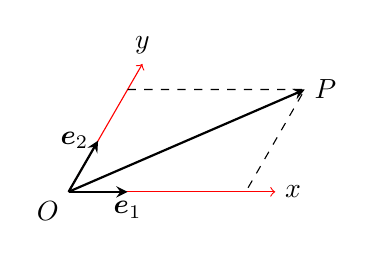
\begin{tikzpicture}[line join=round, scale=0.75]
\coordinate[label=below left:{$O$}]           (O)  at (0,0);
\coordinate[label=below:{$\boldsymbol{e}_1$}] (E1) at (1,0);
\coordinate[label=left: {$\boldsymbol{e}_2$}] (E2) at (0.5,0.866);
\coordinate[label=right:{$x$}]                (x)  at ($(O)!3.5!(E1)$);
\coordinate[label=above:{$y$}]                (y)  at ($(O)!2.5!(E2)$);
\draw[->,red] (O)--(x);
\draw[->,red] (O)--(y);
\draw[thick,-stealth] (O)--(E1);
\draw[thick,-stealth] (O)--(E2);
\coordinate                    (Px) at ($(O)!3!(E1)$);
\coordinate                    (Py) at ($(O)!2!(E2)$);
\coordinate[label=right:{$P$}] (P)  at ($(Px)+(Py)$);
\draw[thick,-stealth] (O)--(P);
\draw[dashed] (Py)--(P)--(Px);
\end{tikzpicture}
\end{figure}

解:

(1)当前坐标系不是正交坐标系,所以$\left| \overrightarrow{OP} \right|\ne 3^2+2^2$,而是需要转换到正交坐标系。
\begin{align*}
&\because \begin{cases}
	\boldsymbol{e}_1=1\cdot \boldsymbol{i}+0\cdot \boldsymbol{j}\\
	\boldsymbol{e}_2=\frac{1}{2}\cdot \boldsymbol{i}+\frac{\sqrt{3}}{2}\cdot \boldsymbol{j}\\
\end{cases} \\
&\therefore \overrightarrow{OP}=3\boldsymbol{e}_1+2\boldsymbol{e}_2=3\left( 1\cdot \boldsymbol{i}+0\cdot \boldsymbol{j} \right) +2\left( \frac{1}{2}\cdot \boldsymbol{i}+\frac{\sqrt{3}}{2}\cdot \boldsymbol{j} \right) =4\boldsymbol{i}+\sqrt{3}\boldsymbol{j} \\
&\therefore \left| \overrightarrow{OP} \right|=\sqrt{4^2+\sqrt{3}^2}
\end{align*}

(2)合理,不展开,XML。

\begin{tcolorbox}
本题考察向量的模的定义,由于教材缺乏明确定义,所以会有些迷惑。
\end{tcolorbox}

~

\begin{example}[拓广探索16,难度:$\star \star $]
用向量方法证明:对于任意的$a,b,c,d\in \mathbb{R} $,恒有不等式
\[
\left( ac+bd \right) ^2\leqslant \left( a^2+b^2 \right) \left( c^2+d^2 \right)
\]
\end{example}

解:

令$\boldsymbol{a}=\left( a,b \right) ,\boldsymbol{b}=\left( c,d \right) $则,
\begin{align*}
&\left( a^2+b^2 \right) \left( c^2+d^2 \right) =\left| \boldsymbol{a} \right|^2\cdot \left| \boldsymbol{b} \right|^2 \\
&\left( \boldsymbol{a}\cdot \boldsymbol{b} \right) ^2=\left( ac+bd \right) ^2
\end{align*}
于是:
\begin{align*}
&\because \cos \alpha =\frac{\boldsymbol{a}\cdot \boldsymbol{b}}{\left| \boldsymbol{a} \right|\cdot \left| \boldsymbol{b} \right|}\in \left[ -1,1 \right] \\
&\therefore \frac{\left( \boldsymbol{a}\cdot \boldsymbol{b} \right) ^2}{\left| \boldsymbol{a} \right|^2\cdot \left| \boldsymbol{b} \right|^2}\in \left[ 0,1 \right]
\end{align*}
当且仅当$\boldsymbol{a},\boldsymbol{b}$平行时等号成立。

\begin{tcolorbox}
本题需要一些想象力,如果没有提示用向量方法,还是有些难度的。
\end{tcolorbox}

\begin{tcolorbox}
这里引申出一个话题。我们在规定向量的坐标$\boldsymbol{a}=\left( x,y \right) $时,并没有对两个坐标量有所约束,更没有要求坐标系必须是直角坐标。加之向量运算的底层规则还是建立在实数的运算法则上,所以本题可以用向量的方法。
\end{tcolorbox}






\newpage
\section{平面向量的应用}

本节要点:
\begin{itemize}
    \item 熟练掌握余弦定理;
    \item 熟练掌握正弦定理。
\end{itemize}

\begin{align*}
&\cos A=\frac{b^2+c^2-a^2}{2bc} \\
&\frac{a}{\sin A}=\frac{b}{\sin B}=\frac{c}{\sin C}
\end{align*}

~

\begin{example}[复习巩固3,难度:$\star $]
用向量法证明:直径所对的圆周角是直角。
\end{example}

解:

如下设置各变量。

\begin{figure}[h]
\centering
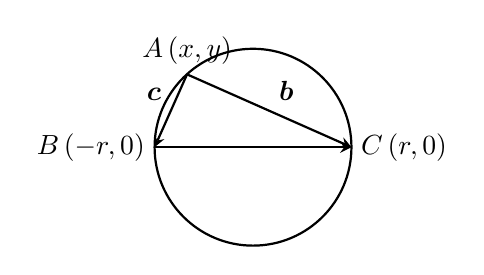
\begin{tikzpicture}[line join=round, scale=1.25]
\mydrawxy{-1.2}{2}{-1.2}{1.2}
\draw[thick] (0,0) circle(1);
\coordinate                                              (O) at (0,0);
\coordinate[label=above:      {$A\left( x,y \right) $}]  (A) at (-0.67,0.74);
\coordinate[label=left:       {$B\left( -r,0 \right) $}] (B) at (-1,0);
\coordinate[label=right:      {$C\left( r,0 \right) $}]  (C) at (1,0);
\coordinate[label=above left: {$\boldsymbol{c}$}]        (c) at ($(A)!0.5!(B)$);
\coordinate[label=above right:{$\boldsymbol{b}$}]        (b) at ($(A)!0.5!(C)$);
\draw[thick,-stealth] (A)--(B);
\draw[thick,-stealth] (A)--(C);
\draw[thick,-stealth] (B)--(C);
\end{tikzpicture}
\end{figure}

\begin{align*}
&\because \begin{cases}
	\boldsymbol{c}=\left( -r-x,-y \right)\\
	\boldsymbol{b}=\left( r-x,-y \right)\\
	x^2+y^2=r^2\\
\end{cases} \\
&\therefore \boldsymbol{c}\cdot \boldsymbol{b}=\left( -r-x \right) \cdot \left( r-x \right) +\left( -y \right) ^2=\left( x^2-r^2 \right) +y^2=0
\end{align*}

\begin{tcolorbox}
本题就是考察垂直的向量表示,也即内积为0的几何意义,较为简单。
\end{tcolorbox}

~

\begin{example}[综合运用15,难度:$\star $]
$\bigtriangleup ABC$的三边分别为$a,b,c$,边$BC$,$CA$,$AB$上的中线分别记为$m_a,m_b,m_c$,利用余弦定理证明
\begin{align*}
&m_a=\frac{1}{2}\sqrt{2\left( b^2+c^2 \right) -a^2} \\
&m_b=\frac{1}{2}\sqrt{2\left( a^2+c^2 \right) -b^2} \\
&m_c=\frac{1}{2}\sqrt{2\left( a^2+b^2 \right) -c^2}
\end{align*}
\end{example}

解一,用余弦定理证明:

\begin{figure}[h]
\centering
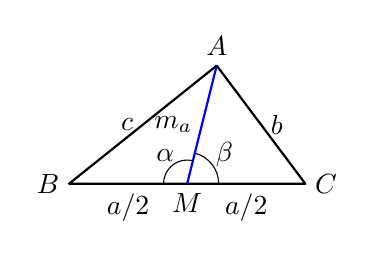
\begin{tikzpicture}[line join=round, scale=0.75]
\coordinate[label=above:{$A$}]   (A)  at (0.5,2);
\coordinate[label=left: {$B$}]   (B)  at (-2,0);
\coordinate[label=right:{$C$}]   (C)  at (2,0);
\coordinate[label=below:{$M$}]   (M)  at ($(B)!0.5!(C)$);
\coordinate[label=right:{$b$}]   (b)  at ($(A)!0.5!(C)$);
\coordinate[label=left: {$c$}]   (c)  at ($(A)!0.5!(B)$);
\coordinate[label=below:{$a/2$}] (a1) at ($(M)!0.5!(B)$);
\coordinate[label=below:{$a/2$}] (a2) at ($(M)!0.5!(C)$);
\coordinate[label=left: {$m_a$}] (ma) at ($(M)!0.5!(A)$);
\draw[thick] (A)--(B)--(C)--(A);
\draw[thick,blue] (A)--(M);
\pic["$\alpha $",draw,angle radius=0.3cm,angle eccentricity=1.5] {angle=A--M--B};
\pic["$\beta $",draw,angle radius=0.4cm,angle eccentricity=1.5] {angle=C--M--A};
\end{tikzpicture}
\end{figure}

如上图,从$\sin \left( \alpha +\beta \right) =\sin \alpha \cos \beta +\cos \alpha \sin \beta =0$开始。

分别使用余弦定理和正弦定理可得:
\[
\frac{c}{m_a}\sin B\cdot \frac{\frac{a^2}{4}+{m_a}^2-b^2}{2\cdot \frac{a}{2}\cdot m_a}+\frac{\frac{a^2}{4}+{m_a}^2-c^2}{2\cdot \frac{a}{2}\cdot m_a}\cdot \frac{b}{m_a}\sin C=0
\]
然后对$\sin B,\sin C$使用正弦定理可得:
\[
\frac{c}{m_a}\cdot \frac{\frac{a^2}{4}+{m_a}^2-b^2}{2\cdot \frac{a}{2}\cdot m_a}+\frac{\frac{a^2}{4}+{m_a}^2-c^2}{2\cdot \frac{a}{2}\cdot m_a}\cdot \frac{b}{m_a}\frac{c}{b}=0
\]
化简:
\[
\frac{a^2}{2}+2{m_a}^2-b^2-c^2=0
\]
略。

\begin{tcolorbox}
本题在于计算量非常大,先要找到合适的角,反反复复找角的过程计算量非常大。
\end{tcolorbox}

解二:

若不限制余弦定理,参考P39的例2,秒答,即证明:
\[
\left( 2m_a \right) ^2+a^2=2\left( b^2+c^2 \right)
\]

~

\begin{example}[综合运用17,难度:$\star \star $]
证明:设三角形的外接圆的半径是$R$,则$a=2R\sin A,b=2R\sin B,c=2R\sin C$。
\end{example}

解:

利用圆心角和圆周角的关系$\angle BOC=2\angle BAC$,加之$\cos 2A=1-\sin ^2A$,可得:
\begin{align*}
&\frac{R^2+R^2-a^2}{2RR}=1-2\sin ^2A \\
&1-\frac{a^2}{2R^2}=1-2\sin ^2A
\end{align*}
后略。

\begin{figure}[h]
\centering
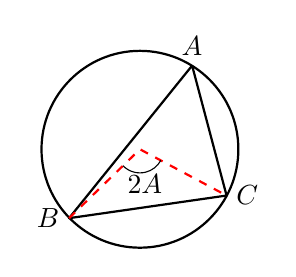
\begin{tikzpicture}[line join=round, scale=1.25]
\draw[thick] (0,0) circle(1);
\coordinate                    (O) at (0,0);
\coordinate[label=above:{$A$}] (A) at (0.53,0.85);
\coordinate[label=left: {$B$}] (B) at (-0.72,-0.7);
\coordinate[label=right:{$C$}] (C) at (0.88,-0.47);
\draw[thick] (A)--(B)--(C)--(A);
\draw[thick,dashed,red] (B)--(O)--(C);
\pic["$2A$",draw,angle radius=0.3cm,angle eccentricity=1.5] {angle=B--O--C};
\end{tikzpicture}
\end{figure}

\begin{tcolorbox}
本题需要结合几何,不能纯靠向量知识,需要一定联想力。
\end{tcolorbox}

~

\begin{example}[拓广探索19,难度:$\star $]
如图,在平行四边形$ABCD$中,点$E,F$分别是$AD,DC$边的中点,$BE,BF$分别与$AC$交于$R,T$两点,你能发现$AR,RT,TC$之间的关系吗?用向量方法证明你的结论。
\end{example}

解:

初看似乎三条线段等长,最直观的方法就是建立如下坐标系,求$R$点的坐标。

\begin{figure}[h]
\centering
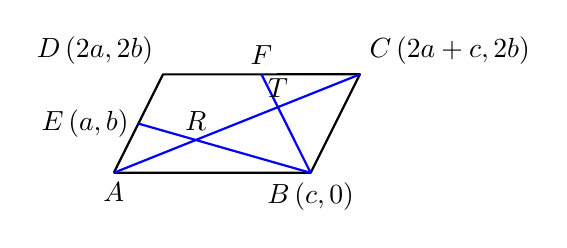
\begin{tikzpicture}[line join=round, scale=1.25]
\mydrawxy{-0.5}{3}{-0.5}{1.5}
\coordinate[label=below:      {$A$}]     (A) at (0,0);
\coordinate[label=below:      {$B\left( c,0 \right) $}]     (B) at (2,0);
\coordinate[label=above left: {$D\left( 2a,2b \right) $}]   (D) at (0.5,1);
\coordinate[label=above right:{$C\left( 2a+c,2b \right) $}] (C) at ($(B)+(D)$);
\coordinate[label=left:       {$E\left( a,b \right) $}]     (E) at ($(A)!0.5!(D)$);
\coordinate[label=above:      {$F$}]                        (F) at ($(D)!0.5!(C)$);
\draw[thick] (A)--(B)--(C)--(D)--(A);
\draw[thick,blue,name path=l1] (A)--(C);
\draw[thick,blue,name path=l2] (B)--(E);
\draw[thick,blue,name path=l3] (B)--(F);
\path [name intersections={of=l1 and l2}] coordinate[label=above:$R$] (R) at (intersection-1);
\path [name intersections={of=l1 and l3}] coordinate[label=above:$T$] (T) at (intersection-1);
\end{tikzpicture}
\end{figure}

易得$EB$和$AC$的直线方程:
\begin{align*}
&y-0=\frac{b}{a-c}\cdot \left( x-c \right) \\
&y=\frac{2b}{2a+c}\cdot x
\end{align*}
联立两方程求得$R$点坐标:
\[
R=\left( x,y \right) =\left( \frac{2a+c}{3},\frac{2b}{3} \right)
\]
确实有$AC=3AR$。

$TC$长度的讨论可以将$C$作为原点建立坐标系,略。

\begin{tcolorbox}
对于定量问题,放到坐标系下讨论,除了计算量大点,没啥缺点。
\end{tcolorbox}

~

\begin{example}[拓广探索20,难度:$\star $]
已知$\bigtriangleup ABC$的三个角$A,B,C$的对边分别为$a,b,c$,设$p=\frac{1}{2}\left( a+b+c \right) $,求证:

(1)三角形的面积$S=\sqrt{p\left( p-a \right) \left( p-b \right) \left( p-c \right)}$;

(2)若$r$为三角形的内切圆半径,则
\[
r=\sqrt{\frac{\left( p-a \right) \left( p-b \right) \left( p-c \right)}{p}}
\]

(3)把$BC,CA,AB$上的高分别记为$h_a,h_b,h_c$,则
\begin{align*}
&h_a=\frac{2}{a}\sqrt{p\left( p-a \right) \left( p-b \right) \left( p-c \right)} \\
&h_b=\frac{2}{b}\sqrt{p\left( p-a \right) \left( p-b \right) \left( p-c \right)} \\
&h_c=\frac{2}{c}\sqrt{p\left( p-a \right) \left( p-b \right) \left( p-c \right)}
\end{align*}
\end{example}

解:

(1)三角形面积
\begin{align*}
S&=\frac{1}{2}bc\sin A=\frac{1}{2}bc\sqrt{1-\cos ^2A} \\
&=\frac{1}{2}bc\sqrt{1-\left( \frac{b^2+c^2-a^2}{2bc} \right) ^2} \\
&=\frac{1}{4}\sqrt{a^4-b^4-c^4+2a^2b^2+2a^2c^2+2b^2c^2}
\end{align*}
而$\sqrt{p\left( p-a \right) \left( p-b \right) \left( p-c \right)}$展开后相等,证毕。

(2)以内切圆圆心为基点,将三角形分成3部分,用下面的思路解,略
\[
S_{\bigtriangleup ABC}=S_{\bigtriangleup ABO}+S_{\bigtriangleup AOC}+S_{\bigtriangleup OBC}
\]

\begin{tcolorbox}
本题计算量略大,方法还是很直观的。
\end{tcolorbox}

~

\begin{example}[拓广探索23,难度:$\star \star $]
已知$a,b,c$分别为$\bigtriangleup ABC$三个内角$A,B,C$的对边,且
\[
a\cos C+\sqrt{3}a\sin C-b-c=0
\]
\begin{enumerate}
    \item 求$A$;
    \item 若$a=2$,且$\bigtriangleup ABC$的面积为$\sqrt{3}$,求$b,c$。
\end{enumerate}
\end{example}

\begin{figure}[h]
\centering
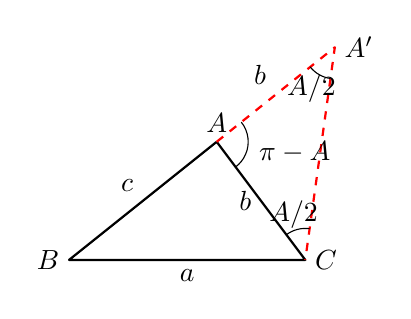
\begin{tikzpicture}[line join=round, scale=0.75]
\coordinate[label=above:     {$A$}]  (A)  at (0.5,2);
\coordinate[label=left:      {$B$}]  (B)  at (-2,0);
\coordinate[label=right:     {$C$}]  (C)  at (2,0);
\coordinate[label=above left:{$c$}]  (c)  at ($(B)!0.5!(A)$);
\coordinate[label=left:      {$b$}]  (b)  at ($(C)!0.5!(A)$);
\coordinate[label=below:     {$a$}]  (a)  at ($(B)!0.5!(C)$);
\coordinate[label=right:     {$A'$}] (A') at ($(B)!1.8!(A)$);
\coordinate[label=above left:{$b$}]  (b') at ($(A)!0.5!(A')$);
\draw[thick] (A)--(B)--(C)--(A);
\draw[thick,dashed,red] (A)--(A')--(C);
\pic["$\pi -A$",draw,angle radius=0.4cm,angle eccentricity=2.5] {angle=C--A--A'};
\pic["$A/2$",draw,angle radius=0.4cm,angle eccentricity=1.5] {angle=A--A'--C};
\pic["$A/2$",draw,angle radius=0.4cm,angle eccentricity=1.5] {angle=A'--C--A};
\end{tikzpicture}
\end{figure}

解:

(1)分析已知等式:
\begin{align*}
&2a\left( \frac{1}{2}\cos C+\frac{\sqrt{3}}{2}\sin C \right) =b+c \\
&2a\sin \left( C+\frac{\pi}{6} \right) =b+c
\end{align*}
出现$\frac{b+c}{a}$,于是构建如上三角形,对$\bigtriangleup A'BC$用正弦定理,并结合已知等式可得:
\begin{align*}
&\because \frac{c+b}{\sin \left( C+\frac{A}{2} \right)}=\frac{a}{\sin \frac{A}{2}} \\
&\therefore \sin \left( C+\frac{A}{2} \right) =\frac{c+b}{a}\sin \frac{A}{2} \\
&\therefore \sin C\cos \frac{A}{2}+\cos C\sin \frac{A}{2}=\frac{c+b}{a}\sin \frac{A}{2} \\
&\therefore \left( a\cot \frac{A}{2} \right) \sin C+a\cos C=b+c \\
&\therefore \cot \frac{A}{2}=\sqrt{3} \\
&\therefore A=\frac{\pi}{3}
\end{align*}

(2)有了$A$,结合三角形公式和余弦定理可得方程组:
\begin{align*}
&\because S=\frac{1}{2}\cdot bc\cdot \sin A=\sqrt{3} \\
&\because \cos A=\frac{b^2+c^2-a^2}{2bc} \\
&\therefore b=c=2
\end{align*}

解二:

从已知等式直接入手:
\begin{align*}
&\because a\cos C+\sqrt{3}a\sin C-b-c=0 \\
&\therefore a\frac{a^2+b^2-c^2}{2ab}+\sqrt{3}c\sin A=b+c \\
&\therefore \sin A=\frac{2b\left( b+c \right) -\left( a^2+b^2-c^2 \right)}{2\sqrt{3}bc}=\frac{1}{\sqrt{3}}\cdot \left( \cos A+1 \right) \\
&\because \sin ^2A+\cos ^2A=1 \\
&\therefore A=\frac{\pi}{3}
\end{align*}

\begin{tcolorbox}
此题有一定难度,解一需要细心观察,解二计算量大,没啥说的。
\end{tcolorbox}






\newpage
\section{本章小结}

本章介绍了平面上的向量,重点:
\begin{itemize}
    \item 向量的运算及其几何意义;
    \item 余弦定理和正弦定理。
\end{itemize}

向量是一个全新的域,还有下一章的复数,和一贯以来的实数不太一样,所以仅用一章的课时难以适应,需要反复阅读概念、推导定理和性质,并结合几何深入思考。向量是代数和几何的桥梁,所以容易出大题和难题,更需要多读多练。

~

\begin{example}[综合运用15,难度:$\star $]
已知$\bigtriangleup P_1P_2P_3$,向量$\overrightarrow{OP_1},\overrightarrow{OP_2},\overrightarrow{OP_3}$满足条件$\overrightarrow{OP_1}+\overrightarrow{OP_2}+\overrightarrow{OP_3}=\mathbf{0},\left| \overrightarrow{OP_1} \right|=\left| \overrightarrow{OP_2} \right|=\left| \overrightarrow{OP_3} \right|$,求证:$\bigtriangleup P_1P_2P_3$是等边三角形。
\end{example}

解:

即通过已知条件求证$\left| \overrightarrow{P_1P_2} \right|=\left| \overrightarrow{P_2P_3} \right|=\left| \overrightarrow{P_3P_1} \right|$。使用{\it xy}坐标系,两个已知条件可表示为:
\begin{align*}
&\because \overrightarrow{OP_1}+\overrightarrow{OP_2}+\overrightarrow{OP_3}=\mathbf{0} \\
&\therefore \begin{cases}
	\left( x_{P1}-x_O \right) +\left( x_{P2}-x_O \right) +\left( x_{P3}-x_O \right) =0\\
	\left( y_{P1}-y_O \right) +\left( y_{P2}-y_O \right) +\left( y_{P3}-y_O \right) =0\\
\end{cases} \\
&\therefore \begin{cases}
	x_{P1}+x_{P2}+x_{P3}=3x_O\\
	y_{P1}+y_{P2}+y_{P3}=3x_O\\
\end{cases} \\
&\because \left| \overrightarrow{OP_1} \right|=\left| \overrightarrow{OP_2} \right|=\left| \overrightarrow{OP_3} \right| \\
&\therefore \left( x_{P1}-x_O \right) ^2+\left( y_{P1}-y_O \right) ^2=\left( x_{P2}-x_O \right) ^2+\left( y_{P2}-y_O \right) ^2 \\
&=\left( x_{P3}-x_O \right) ^2+\left( y_{P3}-y_O \right) ^2
\end{align*}
将$\left( x_{P1}-x_O \right) ^2+\left( y_{P1}-y_O \right) ^2=\left( x_{P2}-x_O \right) ^2+\left( y_{P2}-y_O \right) ^2$部分展开,并将$x_O,y_O$替换掉可得:
\[
\left( x_{P1}-x_{P3} \right) ^2+\left( y_{P1}-y_{P3} \right) ^2=\left( x_{P2}-x_{P3} \right) ^2+\left( y_{P2}-y_{P3} \right) ^2
\]
余下略。

\begin{tcolorbox}
本题思路还是明确的,计算量偏大而已。
\end{tcolorbox}

~

\begin{example}[综合运用16,难度:$\star $]
如图,已知$\overrightarrow{OA}=\boldsymbol{a},\overrightarrow{OB}=\boldsymbol{b}$,任意点$M$关于点$A$的对称点为$S$,点$S$关于点$B$的对称点为$N$,用$\boldsymbol{a},\boldsymbol{b}$表示向量$\overrightarrow{MN}$。(本题可以运用信息技术发现规律)
\end{example}

\begin{figure}[h]
\centering
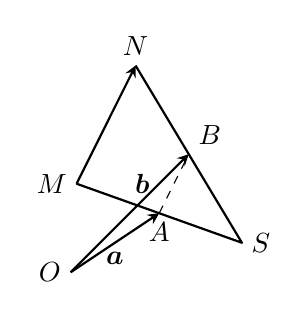
\begin{tikzpicture}[line join=round, scale=0.75]
\coordinate[label=left:       {$O$}]              (O) at (0,0);
\coordinate[label=below:      {$A$}]              (A) at (1.5,1);
\coordinate[label=above right:{$B$}]              (B) at (2,2);
\coordinate[label=left:       {$M$}]              (M) at (0.1,1.5);
\coordinate[label=right:      {$S$}]              (S) at ($(M)!2!(A)$);
\coordinate[label=above:      {$N$}]              (N) at ($(S)!2!(B)$);
\coordinate[label=below:      {$\boldsymbol{a}$}] (a) at ($(O)!0.5!(A)$);
\coordinate[label=left:       {$\boldsymbol{b}$}] (b) at ($(O)!0.75!(B)$);
\draw[thick] (M)--(S)--(N);
\draw[thick,-stealth] (M)--(N);
\draw[thick,-stealth] (O)--(A);
\draw[thick,-stealth] (O)--(B);
\draw[dashed] (A)--(B);
\end{tikzpicture}
\end{figure}

解一:

令$A=\left( x_A,y_A \right) ,B=\left( x_B,y_B \right) ,M=\left( x_M,y_M \right) $,则
\[
\overrightarrow{MN}=\left( x_N-x_M,y_N-y_M \right)
\]
对已知条件整理:
\begin{align*}
&\because \overrightarrow{MS}=2\overrightarrow{AS} \\
&\therefore \begin{cases}
	x_S-x_M=2\left( x_S-x_A \right)\\
	y_S-y_M=2\left( y_S-y_A \right)\\
\end{cases} \\
&\because \overrightarrow{SN}=2\overrightarrow{SB} \\
&\therefore \begin{cases}
	x_N-x_S=2\left( x_B-x_S \right)\\
	y_N-y_S=2\left( y_B-y_S \right)\\
\end{cases} \\
&\therefore \begin{cases}
	x_N-x_M=2\left( x_B-x_A \right)\\
	y_N-y_M=2\left( y_B-y_A \right)\\
\end{cases} \\
&\therefore \overrightarrow{MN}=2\left( x_B-x_A,y_B-y_A \right) =2\left( \boldsymbol{b}-\boldsymbol{a} \right)
\end{align*}

解二:

添加辅助线$AB$,从三角形不难得到$\overrightarrow{MN}=2\overrightarrow{AB}$,余下略。

\begin{tcolorbox}
解一纯用坐标系,思路简单,计算量大。解二结合几何,计算量小。
\end{tcolorbox}










\chapter{复数}

本章介绍复数。难点和平面向量一样,所以依然是反复研读定义,多画图。其次要注意和向量的区别。

本章要点:
\begin{itemize}
    \item 复数及其几何意义。
\end{itemize}

\newpage
\section{复数的概念}

本节要点:
\begin{itemize}
    \item 掌握复数的概念;
    \item 熟悉复数的几何意义;
    \item 理解复数和向量的关系。
\end{itemize}

~

\[
z=a+bi
\]

复数的定义没啥难点,数学家已经帮我们起头了。复数的发明XML。

复数的几何意义对应一个二维平面,但特别注意,由于复数的乘法和向量的乘法(内积)定义不同,所以复数和向量不是同构的,因此,我们称复数的几何表示为复平面,称向量的几何表示为二维平面!XML。

学习到这里一定要注意区别复数和向量。

\begin{tcolorbox}
复数的物理意义需要在解微分方程时讨论,超出高中数学的范围,所以高中阶段不讨论复数的物理意义。我们需要知道,复数确实有物理意义,很多物理现象都涉及复数,XML。
\end{tcolorbox}

~

\begin{example}[拓广探索11,难度:$\star $]
在复平面内指出与复数$z_1=1+2i,z_2=\sqrt{2}+\sqrt{3}i,z_3=\sqrt{3}-\sqrt{2}i,z_4=-2+i$对应的点$z_1,z_2,z_3,z_4$,判断这4个点是否在同一个圆上,并证明你的结论。
\end{example}

解:

在同一个圆上,且圆心为原点。
\[
\left| z_1 \right|=\left| z_2 \right|=\left| z_3 \right|=\left| z_4 \right|=\sqrt{5}
\]

\begin{tcolorbox}
此题非常放水,圆心在原点,直接判断模,非常简单。
\end{tcolorbox}






\newpage
\section{复数的四则运算}

本节要点:
\begin{itemize}
    \item 掌握复数的运算法则;
    \item 理解复数运算的几何意义。
\end{itemize}

~

复数的加减和向量加减一样,但乘除和向量完全不同。
\begin{align*}
&z_1\pm z_2=\left( a_1\pm a_2 \right) +\left( b_1\pm b_2 \right) i \\
&z_1\cdot z_2=\left( a_1+b_1i \right) \cdot \left( a_2+b_2i \right) =\left( a_1a_2-b_1b_2 \right) +\left( a_1b_2+a_2b_1 \right) i
\end{align*}

加法的交换律和结合律:
\begin{align*}
&z_1+z_2=z_2+z_1 \\
&\left( z_1+z_2 \right) +z_3=z_1+\left( z_2+z_3 \right)
\end{align*}

数乘的结合律和分配律:
\begin{align*}
&\lambda \left( \mu z \right) =\left( \lambda \mu \right) z \\
&\left( \lambda +\mu \right) z=\lambda z+\mu z \\
&\lambda \left( z_1+z_2 \right) =\lambda z_1+\lambda z_2
\end{align*}

乘法的交换律、结合律和分配律:
\begin{align*}
&z_1z_2=z_2z_1 \\
&\left( z_1z_2 \right) z_3=z_1\left( z_2z_3 \right) \\
&z_1\left( z_2+z_3 \right) =z_1z_2+z_1z_3
\end{align*}

一个重要的不等式和一个重要的等式:
\begin{itemize}
    \item $\left| z_1+z_2 \right|\leqslant \left| z_1 \right|+\left| z_2 \right|$,当且仅当$z_1,z_2$重叠时等号成立;
    \item $\left| z_1\cdot z_2 \right|=\left| z_1 \right|\cdot \left| z_2 \right|$。
\end{itemize}
注意和向量的区别。






\newpage
\section{复数的三角表示}

本节要点:
\begin{itemize}
    \item 用三角表示理解复数的乘除。
\end{itemize}

~

三角表示及乘除运算如下:
\begin{align*}
&z=a+bi=r\left( \cos \theta +i\sin \theta \right) \\
&z_1\cdot z_2=r_1r_2\left[ \cos \left( \theta _1+\theta _2 \right) +i\sin \left( \theta _1+\theta _2 \right) \right] \\
&\frac{z_1}{z_2}=\frac{r_1}{r_2}\left[ \cos \left( \theta _1-\theta _2 \right) +i\sin \left( \theta _1-\theta _2 \right) \right]
\end{align*}
显然,复数的乘除的几何意义在于旋转。

~

\begin{example}[拓广探索9,难度:$\star $]
如下图,复平面内的$\bigtriangleup ABC$是等边三角形,它的两个顶点$A,B$的坐标分别为$\left( 1,0 \right) ,\left( 2,1 \right) $,求点$C$的坐标。
\end{example}

\begin{figure}[h]
\centering
\begin{minipage}{.49\textwidth}
\centering
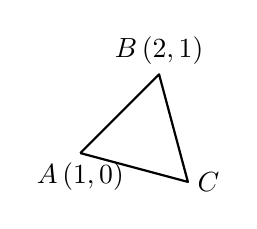
\begin{tikzpicture}[line join=round, scale=1]
\mydrawxy{-0.5}{3}{-0.5}{1.3}
\coordinate[label=below:{$A\left( 1,0 \right) $}] (A) at (1,0);
\coordinate[label=above:{$B\left( 2,1 \right) $}] (B) at (2,1);
\coordinate[label=right:{$C$}]                    (C) at (2.366,-0.366);
\draw[thick] (A)--(B)--(C)--(A);
\end{tikzpicture}
\end{minipage}
\begin{minipage}{.49\textwidth}
\centering
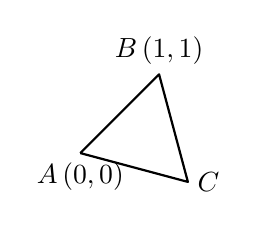
\begin{tikzpicture}[line join=round, scale=1]
\mydrawxy{-0.5}{2}{-0.5}{1.3}
\coordinate[label=below:{$A\left( 0,0 \right) $}] (A) at (0,0);
\coordinate[label=above:{$B\left( 1,1 \right) $}] (B) at (1,1);
\coordinate[label=right:{$C$}]                    (C) at (1.366,-0.366);
\draw[thick] (A)--(B)--(C)--(A);
\end{tikzpicture}
\end{minipage}
\end{figure}

解:

不妨平移坐标,如上右图,不难得到:
\begin{align*}
&z_B=\sqrt{2}\left( \cos \frac{\pi}{4}+i\sin \frac{\pi}{4} \right) \\
&z_C=\sqrt{2}\left[ \cos \left( -\frac{\pi}{12} \right) +i\sin \left( -\frac{\pi}{12} \right) \right]
\end{align*}
$C$在第四象限,于是:
\begin{align*}
&\cos \left( -\frac{\pi}{12} \right) =\sqrt{\frac{1+\cos \frac{\pi}{6}}{2}}=\sqrt{\frac{1}{2}+\frac{\sqrt{3}}{4}} \\
&\sin \left( -\frac{\pi}{12} \right) =-\sqrt{\frac{1-\cos \frac{\pi}{6}}{2}}=-\sqrt{\frac{1}{2}-\frac{\sqrt{3}}{4}} \\
&z_C=\sqrt{1+\frac{\sqrt{3}}{2}}-\sqrt{1-\frac{\sqrt{3}}{2}}i
\end{align*}
将坐标轴反向移回,得到$C$的最终坐标:
\[
z_C=\sqrt{1+\frac{\sqrt{3}}{2}}+1-\sqrt{1-\frac{\sqrt{3}}{2}}i
\]

\begin{tcolorbox}
本题也可以用向量求解,关键在于平移坐标系降低运算量。
\end{tcolorbox}

~

\begin{example}[拓广探索10,难度:$\star $]
如下图,已知平面内并列的三个全等的正方形,利用复数证明
\[
\angle 1+\angle 2+\angle 3=\frac{\pi}{2}
\]
\end{example}

\begin{figure}[h]
\centering
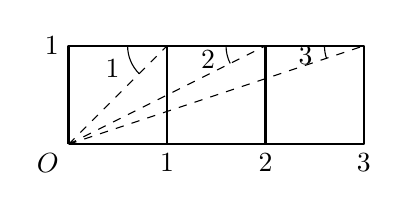
\begin{tikzpicture}[line join=round, scale=1.25]
\mydrawxy{-0.5}{3.5}{-0.5}{1.3}
\coordinate[label=below left:{$O$}] (A0) at (0,0);
\coordinate[label=below:     {$1$}] (A1) at (1,0);
\coordinate[label=below:     {$2$}] (A2) at (2,0);
\coordinate[label=below:     {$3$}] (A3) at (3,0);
\coordinate[label=left:      {$1$}] (B0) at (0,1);
\coordinate                         (B1) at (1,1);
\coordinate                         (B2) at (2,1);
\coordinate                         (B3) at (3,1);
\draw[thick] (A0)--(A3)--(B3)--(B0)--(A0) (A1)--(B1) (A2)--(B2) (A3)--(B3);
\draw[dashed] (A0)--(B1) (A0)--(B2) (A0)--(B3);
\pic["$1$",draw,angle radius=0.5cm,angle eccentricity=1.5] {angle=B0--B1--A0};
\pic["$2$",draw,angle radius=0.5cm,angle eccentricity=1.5] {angle=B0--B2--A0};
\pic["$3$",draw,angle radius=0.5cm,angle eccentricity=1.5] {angle=B0--B3--A0};
\end{tikzpicture}
\end{figure}

解:

令$z_1=1+i,z_2=2+i,z_3=3+i$,使用复数乘法的几何意义:
\[
z_1z_2z_3=\left( 1+i \right) \left( 2+i \right) \left( 3+i \right) =10i
\]
证毕。

\begin{tcolorbox}
本题考察复数乘法的几何意义,非常简单。
\end{tcolorbox}






\newpage
\section{本章小结}

本章介绍了复数,重点在于复数的运算及其几何意义。复数也是一个全新的域,同样需要反复阅读概念并结合几何深入思考,同时需要和向量在乘除上的区别。

我们将向量和复数的运算的几何意义归纳如下。

\begin{table}[ht]
\centering
\begin{tabular}{ccc}
    \toprule
     & 向量 & 复数\\
    \midrule
    加减 & 平行四边形对角线 & 平行四边形对角线\\
    乘法 & 判断直角 & 旋转\\
    除法 & 无 & 旋转\\
    \bottomrule
\end{tabular}
\end{table}

根据具体形况,使用向量判断线段关系,还是使用复数计算线段夹角,需要具体问题具体分析。

~

\begin{example}[拓广探索9,难度:$\star \star \star $]
已知复数
\begin{align*}
&z_1=m+\left( 4-m^2 \right) i \qquad m\in \mathbb{R} \\
&z_2=2\cos \theta +\left( \lambda +3\sin \theta \right) i \qquad \lambda ,\theta \in \mathbb{R}
\end{align*}
并且$z_1=z_2$,求$\lambda $的取值范围。
\end{example}

解:

先考察两个复数的几何图形,均是参数方程,转化为普通方程:
\begin{align*}
&z_1:\begin{cases}
	x=m\\
	y=4-m^2\\
\end{cases}\Rightarrow \quad y=4-x^2 \\
&z_2:\begin{cases}
	x=2\cos \theta\\
	y=\lambda +3\sin \theta\\
\end{cases}\Rightarrow \quad \left( \frac{x}{2} \right) ^2+\left( \frac{y-\lambda}{3} \right) ^2=1
\end{align*}
一个开口向下的抛物线,一个椭圆。$\lambda $控制了椭圆的沿{\it y}轴的平移,要使$z_1=z_2$,即两个图形要相交,$x,y$均需有实数解。几何意义虽然明显,但全靠几何求解很难,考察代数方法,上式带入下式得到:
\[
\frac{4-y}{4}+\left( \frac{y-\lambda}{3} \right) ^2=1
\]
$y$必须在$y\leqslant 4$有实数解
\begin{align*}
&\frac{4-y}{4}+\left( \frac{y-\lambda}{3} \right) ^2=1 \\
&4y^2-\left( 8\lambda +9 \right) y+4\lambda ^2=0 \\
&\because \Delta =\left( 8\lambda +9 \right) ^2-64\lambda ^2\geqslant 0 \\
&\therefore \lambda \geqslant -\frac{9}{16}
\end{align*}
另一个可由几何获得:
\[
\lambda _{\max}=4+3=7
\]
综合得到$\lambda \in \left[ -\frac{9}{16},7 \right] $。

\begin{figure}[h]
\centering
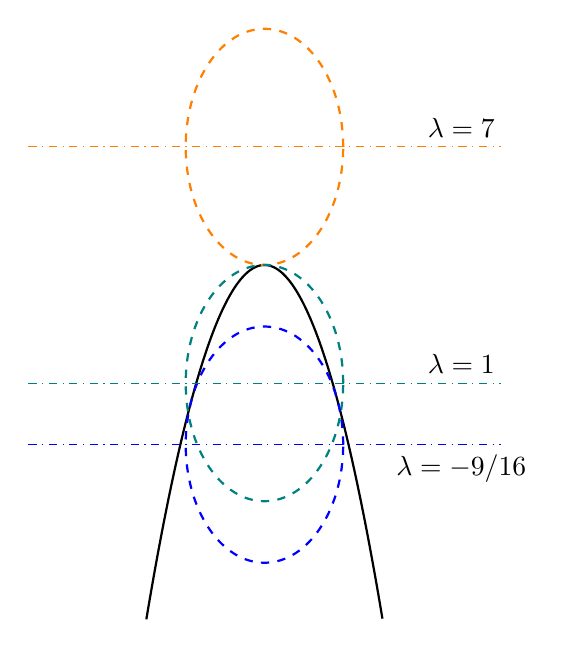
\begin{tikzpicture}[line join=round, scale=0.5]
\mydrawxy{-7}{7}{-5}{11}
\draw[thick,domain=-3:3,samples=200] plot ( \x,{4-((\x)^2)});
\draw[thick,dashed,orange] (0,7)       ellipse (2 and 3);
\draw[thick,dashed,teal]   (0,1)       ellipse (2 and 3);
\draw[thick,dashed,blue]   (0,-0.5625) ellipse (2 and 3);
\draw[dashdotted,orange] (-6,7)--(6,7);
\draw[dashdotted,teal] (-6,1)--(6,1);
\draw[dashdotted,blue] (-6,-0.5625)--(6,-0.5625);
\coordinate[label=above:{$\lambda =7$}]     (t1) at (5,7);
\coordinate[label=above:{$\lambda =1$}]     (t2) at (5,1);
\coordinate[label=below:{$\lambda =-9/16$}] (t3) at (5,-0.5625);
\end{tikzpicture}
\end{figure}

这里附带讨论交点的{\it y}坐标,如下:
\[
y=\frac{\left( 8\lambda +9 \right) \pm 3\sqrt{16\lambda +9}}{8}
\]
\begin{itemize}
    \item $\lambda <-9/16$:$y$没有实数解,两条曲线没有交点;
    \item $\lambda =-9/16$:$y_{1,2}=9/16$,两条曲线有左右2个对称的交点;
    \item $\lambda \in \left( -\frac{9}{16},1 \right) $:$y_{1,2}>0$,两条曲线有左右4个对称的交点;
    \item $\lambda =1$:$y_{1,2}=4,1/4$,两条曲线有左右2个对称的交点,和一个$\left( 0,4 \right) $,共3个交点;
    \item $\lambda \in \left( 1,7 \right) $:$y$有正有负,受$x$实数限制,取$y>0$,所以两条曲线有左右2个对称的交点;
    \item $\lambda =7$:$y_{1,2}=\frac{98}{8},4$,受$x$实数限制,取$y=4$,两条曲线只有顶部1个交点。
\end{itemize}


\begin{tcolorbox}
本题其实考察曲线的交点,结合了复数、参数方程、抛物线、椭圆。纯粹用代数非常复杂,结合几何意义就非常清晰简单。本题很有典型性,仔细研读讨论部分,XML。
\end{tcolorbox}










\chapter{立体几何初步}

本章从纯几何的角度介绍立体几何。

本章要点:
\begin{itemize}
    \item 基本立体图形。
    \item 简单几何体的表面积和体积。
    \item 直线与平面的关系。
\end{itemize}

\newpage
\section{基本立体图形}

本节要点:
\begin{itemize}
    \item 掌握2大类共7种基本立体图形。
\end{itemize}

~

本节没有难度,和之后的知识点关联度不大,只需掌握7种基本立体图形的本质属性,以能做判断。

\begin{itemize}
    \item 多面体:面,棱,顶点;
    \begin{itemize}
        \item 棱柱:底面,侧面,侧棱,顶点,两个底面全等且平行;
        \item 棱锥:底面,侧面,侧棱,顶点,侧面均为三角形;
        \item 棱台:上底面,下底面,母体为棱锥且上下底面平行;
    \end{itemize}
    \item 旋转体:轴;
    \begin{itemize}
        \item 圆柱:轴,底面,侧面,母线,由矩形旋转得到;
        \item 圆锥:轴,底面,侧面,母线,由直角三角形旋转得到;
        \item 圆台:轴,底面,侧面,母线,母体为圆锥且上下底面平行;
        \item 球:球心,半径,直径。
    \end{itemize}
\end{itemize}






\newpage
\section{立体图形的直观图}

略。






\newpage
\section{简单几何体的表面积与体积}

本节要点:
\begin{itemize}
    \item 掌握7种基本立体图形的表面积计算方法;
    \item 掌握7种基本立体图形的体积计算方法。
\end{itemize}

~

体积公式可以归纳如下:
\begin{itemize}
    \item 棱柱,棱锥,棱台,圆柱,圆锥,圆台:
    \[
    V=\frac{S_{\text{上}}+\sqrt{S_{\text{上}}S_{\text{下}}}+S_{\text{下}}}{3}\cdot h
    \]
    \item 球:
    \[
    V=\frac{4}{3}\pi R^3
    \]
\end{itemize}

\begin{tcolorbox}
棱柱锥台、圆柱锥台的体积公式较为有趣,集中了几何平均和算术平均。
\end{tcolorbox}






\newpage
\section{空间点、直线、平面之间的位置关系}

本节要点:
\begin{itemize}
    \item 掌握确定平面的4种方法。
    \item 掌握直线与平面之间的位置关系。
\end{itemize}

~

三维空间的基本元素可以分为点、线、面,高中阶段讨论的是直线和平面。

8.4.1主要讲了如何确定一个平面:
\begin{itemize}
    \item 三点;
    \item 直线+一点;
    \item 两条相交线;
    \item 两条平行线。
\end{itemize}
这些是解题时,构建平面的方法。

8.4.2主要讲了直线与平面之间的位置关系:
\begin{itemize}
    \item 直线与直线的关系:相交,平行,异面;
    \item 直线与平面的关系:属于,相交,平行;
    \item 平面与平面的关系:相交,平行。
\end{itemize}
教材对线面关系没有明确的定义、定理和性质,但类似的概念点较多,相互间逻辑关系非常复杂。万变不离其宗,还是要从最基本的点面关系出发,体会并深刻理解点面关系,多画图。

~

\begin{example}[综合运用8,难度:$\star $]
如图,$\bigtriangleup ABC$在平面$\alpha $外,$AB\cap \alpha =P,BC\cap \alpha =Q,AC\cap \alpha =R$,求证:$P,Q,R$三点共线。
\end{example}

\begin{figure}[h]
\centering
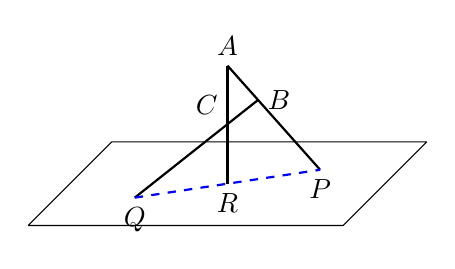
\begin{tikzpicture}[style={x={(-135:0.5)},y={(1cm,0)},z={(0,1cm)}}, line join=round, scale=0.5]
\draw (3,-4,0)--(3,4,0)--(-3,4,0)--(-3,-4,0)--(3,-4,0);
\coordinate[label=below:{$R$}] (R) at (0,0,0);
\coordinate[label=below:{$Q$}] (Q) at (1,-2,0);
\coordinate[label=below:{$P$}] (P) at (-1,2,0);
\coordinate[label=above:{$A$}] (A) at (0,0,3);
\coordinate[label=right:{$B$}] (B) at ($(A)!0.33!(P)$);
\draw[thick] (A)--(P);
\draw[thick,name path=l1] (A)--(R);
\draw[thick,name path=l2] (Q)--(B);
\path [name intersections={of=l1 and l2}] coordinate[label=above left:$C$] (C) at (intersection-1);
\draw[thick,dashed,blue] (Q)--(P);
\end{tikzpicture}
\end{figure}


解:

即找到一个平面,$P,Q,R$三点在该平面上,且该平面和$\alpha $相交。令$\bigtriangleup ABC$所在的平面为$\beta $,则易得$\alpha $和$\beta $相交,令交线为$l$。
\begin{align*}
&\because P\subset AB\Rightarrow P\subset \beta \\
&\because P\subset \alpha \\
&\therefore P\subset \alpha \cap \beta =l
\end{align*}
同理可得$Q,R\subset l$,证毕。

\begin{tcolorbox}
本题看似考察点面关系,实则考察面面关系。
\end{tcolorbox}

~

\begin{example}[拓广探索9,难度:$\star $]
如图是一个正方体的展开图,如果将它还原为正方体,那么在$AB,CD,EF,GH$这四条线段中,哪些线段所在的直线是异面直线?
\end{example}

\begin{figure}[h]
\centering
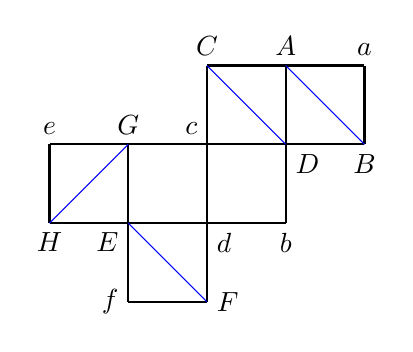
\begin{tikzpicture}[line join=round, scale=1]
\coordinate[label=above:      {$e$}] (e) at (-2,0);
\coordinate[label=above:      {$G$}] (G) at (-1,0);
\coordinate[label=above left: {$c$}] (c) at (0,0);
\coordinate[label=below right:{$D$}] (D) at (1,0);
\coordinate[label=below:      {$B$}] (B) at (2,0);
\coordinate[label=above:      {$C$}] (C) at (0,1);
\coordinate[label=above:      {$A$}] (A) at (1,1);
\coordinate[label=above:      {$a$}] (a) at (2,1);
\coordinate[label=below:      {$H$}] (H) at (-2,-1);
\coordinate[label=below left: {$E$}] (E) at (-1,-1);
\coordinate[label=below right:{$d$}] (d) at (0,-1);
\coordinate[label=below:      {$b$}] (b) at (1,-1);
\coordinate[label=left:       {$f$}] (f) at (-1,-2);
\coordinate[label=right:      {$F$}] (F) at (0,-2);
\draw[thick] (C)--(a) (e)--(B) (H)--(b) (f)--(F);
\draw[thick] (e)--(H) (G)--(f) (C)--(F) (A)--(b) (a)--(B);
\draw[blue] (G)--(H) (E)--(F) (C)--(D) (A)--(B);
\end{tikzpicture}
\end{figure}

解:

需要将展开图还原,标记剩余顶点方便还原,以$dcbD$平面为底,结果如下,余下略。

\begin{figure}[h]
\centering
\begin{tikzpicture}[style={x={(-145:0.5)},y={(1cm,0)},z={(0,1cm)}}, line join=round, scale=2]
\mydrawcube[1]{d}{B}{D}{c}{E}{H}{A}{C}
\draw[blue] (E)--(B)--(A) (H)--(C)--(D);
\coordinate[label=below:{$F$}] (F) at (B);
\coordinate[label=above:{$G$}] (G) at (C);
\end{tikzpicture}
\end{figure}

\begin{tcolorbox}
本题需要空间想象力,较难。还原时,尽量减少翻折次数,以降低难度,所以选$dcbD$平面为底。
\end{tcolorbox}






\newpage
\section{空间直线、平面的平行}

本节要点:
\begin{itemize}
    \item 掌握线面平行的定义;
    \item 掌握线面平行的定理;
    \item 掌握线面平行的性质。
\end{itemize}

~

直线和平面、平面和平面的关系中,重点是平行和垂直关系,本节讨论平行,依照“定义—定理—性质”的步骤理解本节内容。

线面平行:
\begin{itemize}
    \item 定义:直线和平面没有交点;
    \item 定理:若直线和平面内一条直线平行,则线面平行,如下左图;
    \item 性质:若线面平行,则直线和交线平行,如下右图。
\end{itemize}

\begin{figure}[h]
\centering
\begin{minipage}{.49\textwidth}
\centering
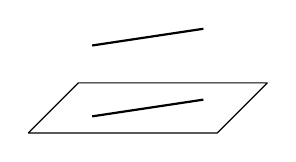
\begin{tikzpicture}[style={x={(-135:0.5)},y={(1cm,0)},z={(0,1cm)}}, line join=round, scale=0.3]
\draw (3,-4,0)--(3,4,0)--(-3,4,0)--(-3,-4,0)--(3,-4,0);
\draw[thick] (1,-2,0)--(-1,2,0) (1,-2,3)--(-1,2,3);
\end{tikzpicture}
\end{minipage}
\begin{minipage}{.49\textwidth}
\centering
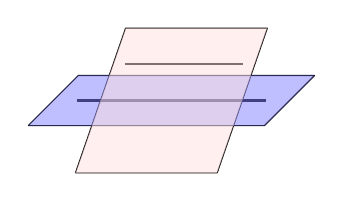
\begin{tikzpicture}[style={x={(-135:0.5)},y={(1cm,0)},z={(0,1cm)}}, line join=round, scale=0.3]
\draw (3,-5,0)--(3,5,0)--(-3,5,0)--(-3,-5,0)--(3,-5,0);
\draw (3,-3,-2)--(3,3,-2)--(-3,3,2)--(-3,-3,2)--(3,-3,-2);
\draw[thick] (0,-4,0)--(0,4,0) (-1.5,-2.5,1)--(-1.5,2.5,1);
\fill[blue!50!white,opacity=0.5] (3,-5,0)--(3,5,0)--(-3,5,0)--(-3,-5,0)--cycle;
\fill[pink!50!white,opacity=0.5] (3,-3,-2)--(3,3,-2)--(-3,3,2)--(-3,-3,2)--cycle;
\end{tikzpicture}
\end{minipage}
\end{figure}

\begin{tcolorbox}
教材对定义和定理讨论较少,倒是对性质给出了证明,反复阅读性质的证明过程P137,领会精神!
\end{tcolorbox}

面面平行:
\begin{itemize}
    \item 定义:平面和平面没有交点;
    \item 定理:若平面内两相交直线和平面平行,则面面平行,如下左图;
    \item 性质:若面面平行,则第三平面产生的两条交线平行,如下右图。
\end{itemize}

\begin{figure}[h]
\centering
\begin{minipage}{.49\textwidth}
\centering
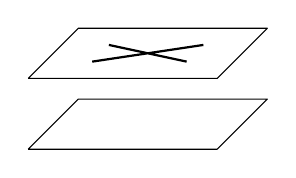
\begin{tikzpicture}[style={x={(-135:0.5)},y={(1cm,0)},z={(0,1cm)}}, line join=round, scale=0.3]
\draw (3,-4,0)--(3,4,0)--(-3,4,0)--(-3,-4,0)--(3,-4,0);
\draw (3,-4,-3)--(3,4,-3)--(-3,4,-3)--(-3,-4,-3)--(3,-4,-3);
\draw[thick] (1,-2,0)--(-1,2,0) (-1,-2,0)--(1,2,0);
\end{tikzpicture}
\end{minipage}
\begin{minipage}{.49\textwidth}
\centering
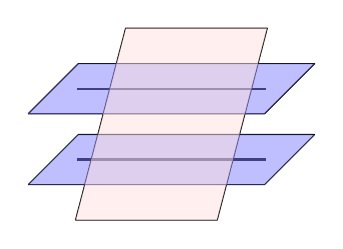
\begin{tikzpicture}[style={x={(-135:0.5)},y={(1cm,0)},z={(0,1cm)}}, line join=round, scale=0.3]
\draw (3,-5,1.5)--(3,5,1.5)--(-3,5,1.5)--(-3,-5,1.5)--(3,-5,1.5);
\draw (3,-5,-1.5)--(3,5,-1.5)--(-3,5,-1.5)--(-3,-5,-1.5)--(3,-5,-1.5);
\draw (3,-3,-3)--(3,3,-3)--(-3,3,3)--(-3,-3,3)--(3,-3,-3);
\draw[thick] (0,-4,1.5)--(0,4,1.5) (0,-4,-1.5)--(0,4,-1.5);
\fill[blue!50!white,opacity=0.5] (3,-5,1.5)--(3,5,1.5)--(-3,5,1.5)--(-3,-5,1.5)--cycle;
\fill[blue!50!white,opacity=0.5] (3,-5,-1.5)--(3,5,-1.5)--(-3,5,-1.5)--(-3,-5,-1.5)--cycle;
\fill[pink!50!white,opacity=0.5] (3,-3,-3)--(3,3,-3)--(-3,3,3)--(-3,-3,3)--cycle;
\end{tikzpicture}
\end{minipage}
\end{figure}

\begin{tcolorbox}
同样,教材对定义和定理讨论较少,对性质的证明过程需要反复阅读P141,领会精神!
\end{tcolorbox}

定义很简单,还没法用于判断,定理用于判断,也称为判断定理。所以解题思路就是先用定理判定平行,然后用性质得出需要的结论。






\newpage
\section{空间直线、平面的垂直}

本节要点:
\begin{itemize}
    \item 掌握异面直线的夹角的定义;
    \item 掌握线面平行的定义;
    \item 掌握线面平行的定理;
    \item 掌握线面平行的性质。
\end{itemize}

~

教材中没有给出异面直线的夹角的明确定义,我们需要领会精神,本质就是通过构造平行线,将异面直线转化为共面直线。所以,所有涉及异面直线夹角的问题,都需要构造平行线,化成共面直线。

本节讨论线面的第二个重点关系,即垂直,依然按照“定义—定理—性质”的步骤理解本节内容。

线面垂直:
\begin{itemize}
    \item 定义:直线和平面内任意直线垂直,注意这里引出的“距离”概念;
    \item 定理:若直线和平面内两条交线垂直,则线面垂直,如下左图;
    \item 性质:若两条直线都和平面垂直,则两条直线平行,如下中图。
\end{itemize}

\begin{figure}[h]
\centering
\begin{minipage}{.32\textwidth}
\centering
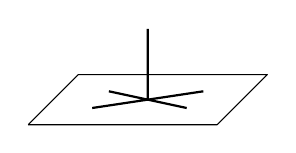
\begin{tikzpicture}[style={x={(-135:0.5)},y={(1cm,0)},z={(0,1cm)}}, line join=round, scale=0.3]
\draw (3,-4,0)--(3,4,0)--(-3,4,0)--(-3,-4,0)--(3,-4,0);
\draw[thick] (1,-2,0)--(-1,2,0) (-1,-2,0)--(1,2,0) (0,0,0)--(0,0,3);
\end{tikzpicture}
\end{minipage}
\begin{minipage}{.32\textwidth}
\centering
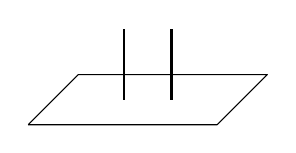
\begin{tikzpicture}[style={x={(-135:0.5)},y={(1cm,0)},z={(0,1cm)}}, line join=round, scale=0.3]
\draw (3,-4,0)--(3,4,0)--(-3,4,0)--(-3,-4,0)--(3,-4,0);
\draw[thick] (0,-1,0)--(0,-1,3) (0,1,0)--(0,1,3);
\end{tikzpicture}
\end{minipage}
\begin{minipage}{.32\textwidth}
\centering
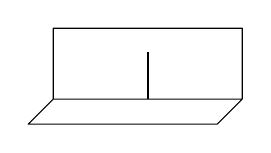
\begin{tikzpicture}[style={x={(-135:0.5)},y={(1cm,0)},z={(0,1cm)}}, line join=round, scale=0.3]
\draw (0,-4,0)--(3,-4,0)--(3,4,0)--(0,4,0)--(0,-4,0)--(0,-4,3)--(0,4,3)--(0,4,0);
\draw[thick] (0,0,0)--(0,0,2);
\end{tikzpicture}
\end{minipage}
\end{figure}

\begin{tcolorbox}
教材对性质的证明使用反证法P153,反复阅读,领会精神!同时注意旁边的框框,它说明了为什么只能用反证法。
\end{tcolorbox}

平平垂直:
\begin{itemize}
    \item 定义:二面角为90°;
    \item 定理:若线面垂直,则平平垂直,如上右图;
    \item 性质:若平平垂直,则垂直于交线的直线构成线面垂直,同如上右图。
\end{itemize}

\begin{tcolorbox}
教材对性质的证明使用二面角的定义P159,反复阅读,领会精神!
\end{tcolorbox}

\begin{tcolorbox}
垂直关系是本章的重点,本节的例5、例7、例8、例10,以及两个性质的证明集中体现了垂直关系的要点,必须反复阅读,领会精神!
\end{tcolorbox}

~

\begin{example}[拓广探索19,难度:$\star $]
如图,在直三棱柱$ABC-A_1B_1C_1$中,$\angle ABC=90^\circ ,AA_1=AB$,求证$A_1C\bot AB_1$。
\end{example}

\begin{figure}[h]
\centering
\begin{minipage}{.49\textwidth}
\centering
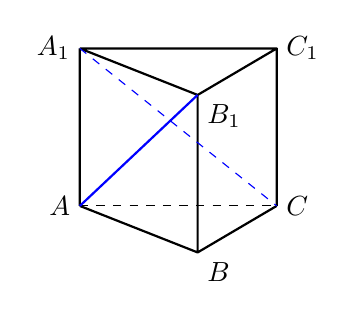
\begin{tikzpicture}[style={x={(-100:0.5)},y={(1cm,0)},z={(0,1cm)}}, line join=round, scale=0.5]
\coordinate[label=left:       {$A$}]   (A)  at (0,0,0);
\coordinate[label=right:      {$C$}]   (C)  at (0,5,0);
\coordinate[label=below right:{$B$}]   (B)  at (2.4,3.2,0);
\coordinate[label=left:       {$A_1$}] (A1) at (0,0,4);
\coordinate[label=right:      {$C_1$}] (C1) at (0,5,4);
\coordinate[label=below right:{$B_1$}] (B1) at (2.4,3.2,4);
\draw[thick] (A1)--(B1)--(C1)--(A1) (A)--(B)--(C) (A)--(A1) (B)--(B1) (C)--(C1);
\draw[dashed] (A)--(C);
\draw[thick,blue] (A)--(B1);
\draw[dashed,blue] (A1)--(C);
\end{tikzpicture}
\end{minipage}
\begin{minipage}{.49\textwidth}
\centering
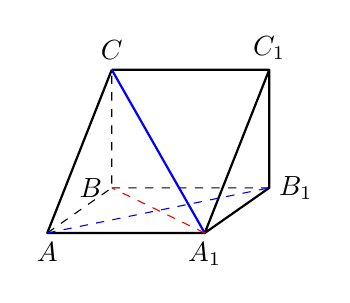
\begin{tikzpicture}[style={x={(-145:0.5)},y={(1cm,0)},z={(0,1cm)}}, line join=round, scale=0.5]
\coordinate[label=left: {$B$}]   (B)  at (0,0,0);
\coordinate[label=below:{$A$}]   (A)  at (4,0,0);
\coordinate[label=above:{$C$}]   (C)  at (0,0,3);
\coordinate[label=right:{$B_1$}] (B1) at (0,4,0);
\coordinate[label=below:{$A_1$}] (A1) at (4,4,0);
\coordinate[label=above:{$C_1$}] (C1) at (0,4,3);
\draw[thick] (C)--(A)--(A1)--(C1)--(C) (A1)--(B1)--(C1);
\draw[dashed] (A)--(B)--(C) (B)--(B1);
\draw[dashed,blue] (A)--(B1);
\draw[thick,blue] (A1)--(C);
\draw[dashed,red] (A1)--(B);
\end{tikzpicture}
\end{minipage}
\end{figure}

解:

原图不容易看,换一下,以$AA_1B_1B$为底,并添辅助线$A_1B$。不难证明线$CB$与面$AA_1B_1B$垂直,于是面$CBA_1$面$AA_1B_1B$垂直,后略。

\begin{tcolorbox}
有时,将立体图形换个角度,有助于发现关键点。
\end{tcolorbox}

~

\begin{example}[拓广探索21,难度:$\star \star $]
如图,在四棱锥$P-ABCD$中,底面$ABCD$为正方形,$PA\bot $底面$ABCD$,$PA=AB$,$E$为线段$PB$的中点,$F$为线段$BC$上的动点。平面$AEF$与平面$PBC$是否相互垂直?如果垂直,请证明;如果不垂直,请说明理由。
\end{example}

\begin{figure}[h]
\centering
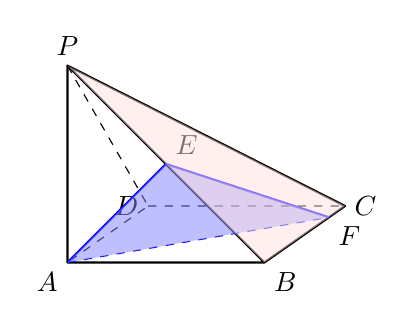
\begin{tikzpicture}[style={x={(-145:0.5)},y={(1cm,0)},z={(0,1cm)}}, line join=round, scale=2.5]
\coordinate[label=above:      {$P$}] (P) at (1,0,1);
\coordinate[label=below left: {$A$}] (A) at (1,0,0);
\coordinate[label=below right:{$B$}] (B) at (1,1,0);
\coordinate[label=right:      {$C$}] (C) at (0,1,0);
\coordinate[label=left:       {$D$}] (D) at (0,0,0);
\coordinate[label=above right:{$E$}] (E) at ($(P)!0.5!(B)$);
\coordinate[label=below right:{$F$}] (F) at ($(B)!0.8!(C)$);
\draw[thick] (B)--(P)--(A)--(B)--(C)--(P);
\draw[dashed] (P)--(D)--(A) (D)--(C);
\draw[thick,blue] (A)--(E)--(F);
\draw[dashed,blue] (A)--(F);
\fill[blue!50!white,opacity=0.5] (A)--(E)--(F)--cycle;
\fill[pink!50!white,opacity=0.5] (B)--(C)--(P)--cycle;
\end{tikzpicture}
\end{figure}

解:

大致过程如下:
\begin{align*}
&\because \bigtriangleup APB\text{为等腰直角}\Rightarrow AE\bot PB \\
&\because CB\bot \text{面}APB\Rightarrow CB\bot AE \\
&\therefore AE\bot \text{面}PCB
\end{align*}

\begin{tcolorbox}
动点$F$可以理解为面$AEF$绕着轴$AE$旋转,就容易理解了。
\end{tcolorbox}






\newpage
\section{本章小结}

本章的重点在线面关系,难点在于垂直关系。线面关系是面面关系的基础,而线线关系又是线面关系的基础。{\bf 所以一切空间关系,归根结底还是平面关系。}解题时需要紧紧抓住这一点,将空间中的点线元素通过平移、作垂线等方法放到同一个平面中讨论。

我们在平面几何中详细讨论了点线面的关系,总结出了相当完善的理论,小到直线平行和垂直,大到三角形相似,甚至有平面向量。所以,要善用已知考察未知,用平面考察立体,牢牢记住{一切空间关系,归根结底还是平面关系。}

%============================================================
\subsection{习题}

\begin{example}[综合运用11,难度:$\star \star \star $]
如下图,在四面体$A-BCD$中,$M$是$AD$的中点,$P$是$BM$的中点,点$Q$在线段$AC$上,且$AQ=3QC$。求证:$PQ\parallel \text{平面}BCD$。
\end{example}

\begin{figure}[h]
\centering
\begin{minipage}{.49\textwidth}
\centering
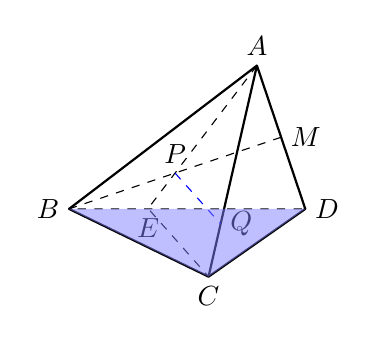
\begin{tikzpicture}[style={x={(-145:0.5)},y={(1cm,0)},z={(0,1cm)}}, line join=round, scale=1.5]
\coordinate[label=above:{$A$}] (A) at (1,1,1.5);
\coordinate[label=left: {$B$}] (B) at (0,-1,0);
\coordinate[label=below:{$C$}] (C) at (2,1,0);
\coordinate[label=right:{$D$}] (D) at (0,1,0);
\coordinate[label=right:{$M$}] (M) at ($(A)!0.5!(D)$);
\coordinate[label=above:{$P$}] (P) at ($(B)!0.5!(M)$);
\coordinate[label=right:{$Q$}] (Q) at ($(A)!0.75!(C)$);
\coordinate[label=below:{$E$}] (E) at ($(A)!1.33!(P)$);
\draw[thick] (A)--(B)--(C)--(A)--(D)--(C);
\draw[dashed] (A)--(E)--(C) (M)--(B)--(D);
\draw[dashed,blue] (P)--(Q);
\fill[blue!50!white,opacity=0.5] (B)--(C)--(D)--cycle;
\end{tikzpicture}
\end{minipage}
\begin{minipage}{.49\textwidth}
\centering
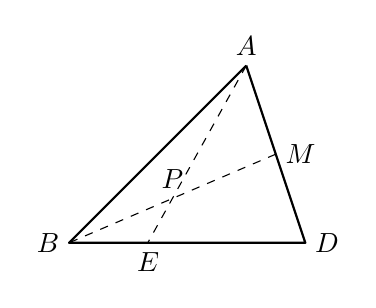
\begin{tikzpicture}[line join=round, scale=1.5]
\coordinate[label=above:{$A$}] (A) at (0.5,1.5);
\coordinate[label=left: {$B$}] (B) at (-1,0);
\coordinate[label=right:{$D$}] (D) at (1,0);
\coordinate[label=right:{$M$}] (M) at ($(A)!0.5!(D)$);
\coordinate[label=above:{$P$}] (P) at ($(B)!0.5!(M)$);
\coordinate[label=below:{$E$}] (E) at ($(A)!1.33!(P)$);
\draw[thick] (A)--(B)--(D)--(A);
\draw[dashed] (A)--(E) (M)--(B);
\end{tikzpicture}
\end{minipage}
\end{figure}

解:

证明线面平行,就是证明线线平行,即在$BCD$中寻找一条线和$PQ$共线,很自然作$AP$并延长交$DB$于$E$。于是只需证明$PQ\parallel EC$即可,由于$AQ=3QC$,也即只需证明$AP=3PE$。将$ABD$单独拉出来,如上右图。最直观的就是使用平面向量,设$A=\left( a,b \right) ,D=\left( c,0 \right) $,则有:
\[
M=\left( \frac{a+c}{2},\frac{b}{2} \right) ,P=\left( \frac{a+c}{4},\frac{b}{4} \right)
\]
可构建直线$AE$的方程,求解得到$E$的坐标:
\[
E=\left( \frac{c}{3},0 \right)
\]
不难发现$\left| \overrightarrow{EA} \right|=4\left| \overrightarrow{EP} \right| $,余下略,证毕。

\begin{tcolorbox}
本题有$AP=3PE$之类不伦不类的数量关系,化到平面使用向量方法是最直观的。
\end{tcolorbox}

~

\begin{example}[综合运用12,难度:$\star \star $]
如图,在正方体$ABCD-A_1B_1C_1D_1$中,求证:
\begin{enumerate}
    \item $B_1D\bot \text{平面}A_1BC_1$;
    \item $B_1D$与平面$A_1BC_1$的交点$H$是$\bigtriangleup A_1BC_1$的重心。
\end{enumerate}
\end{example}

\begin{figure}[h]
\centering
\begin{tikzpicture}[style={x={(-145:0.5)},y={(1cm,0)},z={(0,1cm)}}, line join=round, scale=2]
\pgfmathparse{0.6/2.5}
\mydrawcube[1]{A}{B}{C}{D}{A_1}{B_1}{C_1}{D_1}
\coordinate[label=right:{$E$}] (E) at ($(B)!0.5!(C_1)$);
\draw[thick,blue] (A_1)--(C_1)--(B)--(A_1);
\draw[dashed,blue,name path=l1] (D)--(B_1);
\draw[dashed,red,name path=l2] (A_1)--(E);
\path [name intersections={of=l1 and l2}] coordinate[label=left:$H$] (H) at (intersection-1);
\fill (H) circle (\pgfmathresult mm);
\fill[blue!50!white,opacity=0.5] (A_1)--(C_1)--(B)--cycle;
\end{tikzpicture}
\end{figure}

解:

(1)还是较为简单,大致思路如下。

只需证明$B_1D\bot A_1B$且$B_1D\bot C_1B$且$B_1D\bot A_1C_1$,由于对称性,证明一个即可,可选$B_1D\bot A_1B$。不难证明$A_1B$平行于$B_1D$所在平面$ADC_1B_1$,证毕。

(2)连接$A_1,H$并延长交于$E$,不难发现$\bigtriangleup A_1BC_1$是等边三角形,也即证明$E$平分$BC_1$或$A_1E\bot BC_1$或$\angle C_1A_1E=\angle BA_1E$,观察后发现证明$A_1E\bot BC_1$较为简单。
\begin{align*}
&\because BC_1\bot A_1D \\
&\because BC_1\bot A_1B_1 \\
&\therefore BC_1\bot A_1DEB_1 \\
&\therefore BC_1\bot A_1E
\end{align*}

\begin{tcolorbox}
本题略有复杂,也是典型的空间几何证明题。大致套路就是若要证明线线垂直就先证明线面垂直,要证明线面垂直就先证明线线垂直。
\end{tcolorbox}

~

\begin{example}[综合运用13,难度:$\star $]
如图,在三棱锥$P-ABC$中,$\angle ACB=90^\circ$,$PA\bot \text{底面}ABC$。
\begin{enumerate}
    \item 求证:$\text{平面}PAC\bot \text{平面}PBC$;
    \item 若$AC=BC=PA$,$M$是$PB$的中点,求$AM$与平面$PBC$所成角的正切值。
\end{enumerate}
\end{example}

\begin{figure}[h]
\centering
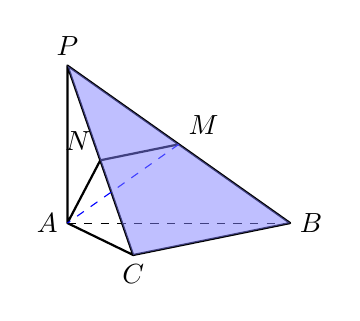
\begin{tikzpicture}[style={x={(-145:0.5)},y={(1cm,0)},z={(0,1cm)}}, line join=round, scale=2]
\coordinate[label=above:       {$P$}] (P) at (0,0,1);
\coordinate[label=left:        {$A$}] (A) at (0,0,0);
\coordinate[label=right:       {$B$}] (B) at (0,1.414,0);
\coordinate[label=below:       {$C$}] (C) at (0.707,0.707,0);
\coordinate[label=above right: {$M$}] (M) at ($(P)!0.5!(B)$);
\coordinate[label=above left:  {$N$}] (N) at ($(P)!0.5!(C)$);
\draw[thick] (P)--(A)--(C)--(B)--(P)--(C) (A)--(N)--(M);
\draw[dashed] (A)--(B);
\draw[dashed,blue] (M)--(A);
\fill[blue!50!white,opacity=0.5] (P)--(C)--(B)--cycle;
\end{tikzpicture}
\end{figure}

解:

(1)略。

(2)关键在于找角,也即找到$A$在平面$PCB$上的垂足。从(1)已知$BC\bot PAC$,所以尽量考虑在$PC$上找一点,设$N$,使得$AN\bot PC$,于是$AN\bot PCB$,也即$N$就是垂足,题目要求的所成角即为$\angle NMA$。不难发现$\bigtriangleup PAC$为等腰直角三角形,于是易得:
\[
\tan \angle NMA=\frac{AN}{NM}=\frac{\sqrt{2}/2}{1/2}=\sqrt{2}
\]

\begin{tcolorbox}
本题关键在于找直线与平面的成角,没有其他方法,只有根据定义找。
\end{tcolorbox}

~

\begin{example}[综合运用14,难度:$\star $]
如图,在四棱锥$P-ABCD$中,底面$ABCD$为正方形,侧面$PAD$是正三角形,$\text{侧面}PAD\bot \text{底面}ABCD$,$M$是$PD$的中点。
\begin{enumerate}
    \item 求证:$AM\bot \text{平面}PCD$;
    \item 求侧面$PBC$与底面$ABCD$所成二面角的余弦值。
\end{enumerate}
\end{example}

\begin{figure}[h]
\centering
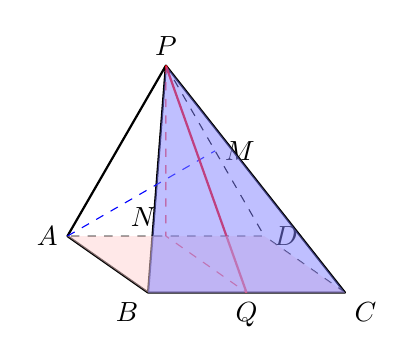
\begin{tikzpicture}[style={x={(-35:0.5)},y={(1cm,0)},z={(0,1cm)}}, line join=round, scale=1.25]
\coordinate[label=above:      {$P$}] (P) at (0,0,1.732);
\coordinate[label=left:       {$A$}] (A) at (0,-1,0);
\coordinate[label=below left: {$B$}] (B) at (2,-1,0);
\coordinate[label=below right:{$C$}] (C) at (2,1,0);
\coordinate[label=right:      {$D$}] (D) at (0,1,0);
\coordinate[label=right:      {$M$}] (M) at ($(P)!0.5!(D)$);
\coordinate[label=above left: {$N$}] (N) at ($(A)!0.5!(D)$);
\coordinate[label=below:      {$Q$}] (Q) at ($(B)!0.5!(C)$);
\draw[thick] (P)--(A)--(B)--(P)--(C)--(B);
\draw[dashed] (P)--(D)--(A) (C)--(D);
\draw[dashed,blue] (A)--(M);
\draw[thick,red] (P)--(Q);
\draw[dashed,red] (P)--(N)--(Q);
\fill[pink!70!white,opacity=0.5] (A)--(D)--(C)--(B)--cycle;
\fill[blue!50!white,opacity=0.5] (P)--(C)--(B)--cycle;
\end{tikzpicture}
\end{figure}

解:

(1)略。

(2)关键在于找二面角,也即在$BC$找一点$Q$,能够方便地作垂线。显然用$P$找$Q$较为方便,不难发现$\bigtriangleup PBC$为等腰三角形,于是很自然$Q$取$BC$中点,再取$AD$中点$N$。不难证明,$\angle NQP$就是要求的二面角,而且$\angle PNQ$是直角,于是:
\[
\cos \angle NQP=\frac{NQ}{PQ}=\frac{1}{\sqrt{7}/2}
\]

\begin{tcolorbox}
本题关键在于找二面角,同上题没有其他方法,只有根据定义找。
\end{tcolorbox}










\chapter{统计}

本章介绍数理统计的3个基础概念,均值、百分位数和方差。本章和下一章的内容一起组成了“概率论”的重要内容,一般来讲,国内讲述概率论的教材,都会分成概率论和数理统计两部分。其中,概率论是理论基础,数理统计是应用。

本章要点:
\begin{itemize}
    \item 均值。
    \item 百分位数。
    \item 方差。
\end{itemize}

\newpage
\section{随机抽样}

本节要点:
\begin{itemize}
    \item 掌握均值的概念;
    \item 理解分层随机抽样。
\end{itemize}

~

本节介绍第一个统计指标,均值,没有难度。均值就是算术平均,我们用样本均值代替总体均值以考察总体的平均水平。

简单随机抽样的特点就是简单,其均值计算就是采用算术平均。分层随机抽样的特点是根据其他的分布特点均化样本,降低相关度,其均值计算是先算术平均,再加权算数平均。






\newpage
\section{用样本估计总体}

本节要点:
\begin{itemize}
    \item 了解概率分布;
    \item 掌握百分位数的概念;
    \item 掌握方差的概念。
\end{itemize}

~

本节介绍了数理统计中的剩余两个重要概念:百分位数(代表性的是中位数)和方差。学习是特别要注意它们的物理意义,XML。

\begin{tcolorbox}
教材中有一处错误。一般来讲,样本的方差应该是
\[
S^2=\frac{\sum_{i=1}^n{\left( X_i-\bar{X} \right)}^2}{n-1}
\]
分母是$n-1$,因为只有这样$S^2$才能是总体方差的无偏估计。而$\frac{1}{n}\sum_{i=1}^n{\left( X_i-\bar{X} \right)}^2$称为样本的2阶中心距。
\end{tcolorbox}






\newpage
\section{统计案例}

略。






\newpage
\section{本章小结}

本章的非常简单地介绍了数理统计,主要掌握三个概念:

\begin{itemize}
    \item 均值:真正名称为“数学期望”,物理意义是质心;
    \item 中位数:物理意义是质量平分,和均值的区别在于无需考虑力矩;
    \item 方差:物理意义是转动惯量。
\end{itemize}










\chapter{概率}

本章介绍概率论的几个基础概念。

本章要点:
\begin{itemize}
    \item 事件。
    \item 古典概型。
    \item 独立性。
\end{itemize}

\newpage
\section{随机事件与概率}

本节要点:
\begin{itemize}
    \item 掌握事件的概念;
    \item 掌握事件的运算;
    \item 掌握古典概型及其概率的计算;
    \item 掌握概率的性质。
\end{itemize}

~

本节介绍概率的一些基础概念,特别要注意几点。

首先事件的运算是逻辑运算,而非算术运算。其次,古典概型是两大概型的一种,另一种是几何概型,笼统来说,古典概型是掰手指,几何概型是量尺子。最后,对概率性质的理解可以从直觉出发,也需结合图形。






\newpage
\section{事件的相互独立性}

本节要点:
\begin{itemize}
    \item 了解独立性的概念。
\end{itemize}

~

独立性是一个很深刻的概念,也是一个非常强的约束条件,反映了事件$A$的发生与否对事件$B$没有影响。其次要注意的是,我们一般不从定义判断两个事件是否独立,而是从事实角度判断,如果两个事件独立,则使用公式
\[
P\left( AB \right) =P\left( A \right) P\left( B \right)
\]
计算。通常而言,如果事件$A$描述了试验$E_A$的结果,事件$B$描述了试验$E_B$的结果,试验$E$由$E_A,E_B$构成,且$E_A,E_B$不存在相互逻辑关系,则$A,B$相互独立。






\newpage
\section{频率与概率}

略。






\newpage
\section{本章小结}

本章的非常简单地介绍了概率论,主要掌握古典概型的概率计算,难点在于独立性的前提下的概率计算。












\end{document}




